\documentclass[sigconf]{acmart}
% \documentclass{...}
%\documentclass[11pt, letterpaper]{article}
\usepackage[margin=1in]{geometry}

% \documentclass[11pt, letterpaper]{article}
% 
% % ----- margins -----
% 
% \topmargin -1.5cm         % read Lamport p.163
% \oddsidemargin -0.04cm    % read Lamport p.163
% \evensidemargin -0.04cm   % same as oddsidemargin but for left-hand pages
% 
% % ----- texts -----
% 
% \textwidth 16.59cm
% \textheight 21.94cm
% 
% % ----- indendts and spacing -----
% 
% \parskip 0pt            	% spacing between paragraphs
% %\renewcommand{\baselinestretch}{1.5}	% uncomment for 1.5 spacing
% 
% \parindent 7mm		      % leading space for paragraphs between lines
% 
% % ----- page # -----
% 
% %\pagestyle{empty}         % uncomment if don't want page numbers





%=== use the these packages if they are not already in use ===
%\usepackage{amsfonts}
%\usepackage{amsmath}
%\usepackage{amssymb}
\usepackage{amsthm}
\usepackage{bbm} 
%\usepackage{cite}
\usepackage{color}
%\usepackage{euscript}
\usepackage{graphicx}
\usepackage{mathrsfs} 
%\usepackage{microtype}
% \usepackage[normalem]{ulem}
% \usepackage{wrapfig}
%=============================================================

%===== control =====
\allowdisplaybreaks

%===== fonts =====
\def\ttt{\texttt}
\def\tsc{\textsc}

%===== spacing =====

\def\extraspacing{\vspace{3mm} \noindent}
\def\figcapup{\vspace{-1mm}}
\def\figcapdown{\vspace{-0mm}}
\def\hgap{\textrm{\hspace{1mm}}}
\def\thmvgap{\vspace{0mm}}
\def\vgap{\vspace{1mm}}


%===== tabbing =====

\def\tab{\hspace{3mm}}
\def\tabpos{\hspace{4mm} \= \hspace{4mm} \= \hspace{4mm} \= \hspace{4mm} \= \hspace{4mm} \= \hspace{4mm} \= \hspace{4mm} \= \hspace{4mm} \= \hspace{4mm} \= \hspace{4mm} \= \hspace{4mm} \= \hspace{4mm} \= \hspace{4mm} \= \hspace{4mm} %\= 
%\= \hspace{4mm} \= \hspace{4mm} \= \hspace{4mm} \= \hspace{4mm} \= \hspace{4mm} \= \hspace{4mm}
\kill}
\newcommand{\mytab}[1]{\begin{tabbing}\tabpos #1\end{tabbing}}

%===== blocks =====

%%%%%%%%%%%%%%%%%%%%%%%%%%%%%%%%
% THEOREMS
%%%%%%%%%%%%%%%%%%%%%%%%%%%%%%%%
% \theoremstyle{plain}
% \newtheorem{theorem}{Theorem}[section]
% \newtheorem{proposition}[theorem]{Proposition}
% \newtheorem{lemma}[theorem]{Lemma}
% \newtheorem{corollary}[theorem]{Corollary}
% \theoremstyle{definition}
% \newtheorem{definition}[theorem]{Definition}
% \newtheorem{assumption}[theorem]{Assumption}
% \theoremstyle{remark}
% \newtheorem{remark}[theorem]{Remark}

% \newtheorem{theorem}{Theorem}
% \newtheorem{lemma}[theorem]{Lemma}
% \newtheorem{corollary}[theorem]{Corollary}
% \newtheorem{proposition}{Proposition}
% \newtheorem{definition}{Definition}
% \newtheorem{problem}{Problem}

\newcommand{\boxminipg}[2]{\begin{center}\fbox{\begin{minipage}{#1}#2\end{minipage}}\end{center}}
\newcommand{\minipg}[2]{\begin{center}\begin{minipage}{#1}#2\end{minipage}\end{center}}
\newcommand{\myitems}[1]{\begin{itemize} #1 \end{itemize}}
\newcommand{\myenums}[1]{\begin{enumerate} #1 \end{enumerate}}
\newcommand{\myfig}[1]{\begin{figure}\centering #1\end{figure}}
\newcommand{\myfigg}[2]{\begin{figure}\centering #1 \figcapup \caption{#2} \figcapdown \end{figure}}
\newcommand{\myfigstar}[2]{\begin{figure*}\centering #1 \figcapup \caption{#2} \figcapdown \end{figure*}}

%===== math macros =====

\newcommand{\bm}[1]{\textrm{\boldmath${#1}$}}
\newcommand{\mb}[1]{\mathbf{#1}}
% \newcommand{\smat}[2]{\left[\begin{tabular}{#1}#2\end{tabular}\right]}
% \newcommand{\bmat}[2]{\left|\begin{tabular}{#1}#2\end{tabular}\right|}
\newcommand{\bmat}[1]{\begin{bmatrix}#1\end{bmatrix}}
\newcommand{\vmat}[1]{\begin{vmatrix}#1\end{vmatrix}}
\newcommand{\myeqn}[1]{\begin{eqnarray}#1\end{eqnarray}}
\newcommand{\myset}[1]{\{#1\}}
\newcommand{\set}[1]{\{#1\}}

\newcommand{\explain}[1]{(\textrm{#1})}
%\newcommand{\bracket}[1]{\left(#1\right)}
%\newcommand{\dbar}[1]{\Vert#1\Vert}
%\newcommand{\one}[1]{\mathbbm{1}\{#1\}}

%\def\bm{\boldmath}
%\def\defeq{\stackrel{\textrm{\tiny{def}}}{=}}
\def\mit{\mathit}
\def\defeq{:=}
\def\eps{\epsilon}
\def\fr{\frac}
\def\-{\mbox{-}}
\def\ol{\overline}
\def\real{\mathbb{R}}
\def\intdom{\mathbb{N}}

\def\tO{\tilde{O}}
\def\tOmega{\tilde{\Omega}}

\def\lc{\left \lceil}
\def\lf{\left \lfloor}
\def\rc{\right \rceil}
\def\rf{\right \rfloor}
\newcommand{\ceil}[1]{\lceil #1 \rceil}
\newcommand{\floor}[1]{\lfloor #1 \rfloor}

\def\nn{\nonumber}

\def\Pr{\mathbf{Pr}}
%\def\expt{\mathbf{E}}
\def\var{\mathbf{Var}}

\def\dcl{\{\!\!\{}
\def\dcr{\}\!\!\}}
\def\bigdcl{\Big\{\!\!\Big\{}
\def\bigdcr{\Big\}\!\!\Big\}}
\def\bigmid{\textrm{ $\Big|$ }}


\DeclareMathOperator*{\argmin}{arg\,min}
\DeclareMathOperator*{\argmax}{arg\,max}
\DeclareMathOperator*{\polylog}{polylog}
\DeclareMathOperator*{\poly}{poly}
\DeclareMathOperator*\expt{\mathbf{E}}
%\DeclareMathOperator*\Pr{\mathbf{Pr}}

%===== misc =====

\def\done{\qed \vspace{2mm}}	% end of proof
\def\tbc{\hspace*{\fill} $\textrm{{\em (to be continued)}}\blacktriangle$ \vspace{2mm}}
%\def\done{\hspace*{\fill} $\Box$}	% end of proof
\allowdisplaybreaks
%===== coloring =====

\newcommand{\red}[1]{\textcolor{red}{#1}}
\newcommand{\blue}[1]{\textcolor{blue}{\bf #1}}
\newcommand{\purple}[1]{\textcolor{purple}{\bf #1}}
\newcommand{\todo}[1]{\textcolor{red}{\bf [TO DO: #1]}}


%=================================
%Yufei's stuff
%\usepackage{amsmath}
\usepackage{balance}
%\usepackage{times}
\usepackage{microtype}

\def\vgap{\vspace{0mm}}
\def\extraspacing{\vspace{1.5mm} \noindent}
\def\figcapup{\vspace{-2mm}}
\def\figcapdown{\vspace{-2mm}}

\def\A{\mathcal{A}}
\def\B{\mathcal{B}}
\def\C{\mathcal{C}}
\def\E{\mathcal{E}}
\def\G{\mathcal{G}}
\def\I{\mathcal{I}}
\def\J{\mathcal{J}}
\def\II{\mathscr{I}}
\def\L{\mathcal{L}}
\def\P{\mathcal{P}}
\def\Q{\mathcal{Q}}
\def\R{\mathcal{R}}
\def\T{\mathcal{T}}
\def\U{\mathcal{U}}
\def\V{\mathcal{V}}
\def\X{\mathcal{X}}
\def\XX{\mathscr{X}}
\def\Y{\mathcal{Y}}
\def\YY{\mathscr{Y}}
\def\Z{\mathcal{Z}}

\def\xleft{\mathrm{left}}
\def\xright{\mathrm{right}}
\def\ybot{\mathrm{bot}}
\def\ytop{\mathrm{top}}
\def\maxtop{\mathrm{maxtop}}
\def\minleft{\mathrm{minleft}}
\def\gleft{\mathrm{left\text{-}guard}}
\def\gbot{\mathrm{bot\text{-}guard}}
\def\cross{\mathrm{cross}}
\def\dcross{\mathrm{d\text{-}cross}}
\def\contained{\mathrm{contained}}
\def\cat{\mathrm{cat1}}
\def\catt{\mathrm{cat2}}
\def\out{\mathrm{OUT}}

\allowdisplaybreaks
%=================================

%====== from acm ======
\acmDOI{}
\acmISBN{}

\acmConference[]{...}{...}{...}
\acmYear{...}
\copyrightyear{}
\acmArticle{}
\acmPrice{}
%======================



\begin{document}
%\begin{sloppy}
    
\title{Optimal (Multiway) Spatial Joins}

% \author{}
% \affiliation{
% 	\institution{Chinese University of Hong Kong}
% 	\city{Hong Kong}
% 	\country{China}}	

\author{}


\begin{abstract}
    In a {\em spatial join}, we are given a constant number $k \geq 2$ of sets containing axis-parallel rectangles in a 2D space, denoted as $R_1, R_2, ..., R_k$. The objective is to report all $k$-tuples $(r_1, r_2, ..., r_k) \in R_1 \times R_2 \times ... \times R_k$ where the rectangles $r_1, r_2, ..., r_k$ have a non-empty intersection, i.e., $r_1 \cap r_2 \cap ... \cap r_k \neq \emptyset$. The problem holds significant importance in spatial databases and has been extensively studied in the database community. In this paper, we show how to settle the problem in $O(n \log n + \out)$ time --- regardless of the constant $k$ --- where $n = \sum_{i=1}^k |R_i|$ and $\out$ is the result size (i.e., the total number of $k$-tuples reported). The runtime  is asymptotically optimal in the class of comparison-based algorithms, to which our solution belongs. Our result significantly improves the state of the art, which is an algorithm with running time $O(n \log^{2k} n + \out)$.
\end{abstract}

\maketitle 

\section{Introduction} \label{sec:intro}

This paper studies the {\em spatial join} (SJ) problem formulated as follows. Let $k \ge 2$ be a constant integer. In the {\em $k$-SJ} problem, the input comprises $k$ sets --- denoted as $R_1, R_2, ..., R_k$ --- of axis-parallel rectangles\footnote{A rectangle is {\em axis-parallel} if it has the form $r = [x_1, x_2] \times [y_1, y_2]$.} in $\real^2$. The goal is to find all $k$-tuples $(r_1, r_2, ..., r_k)$ where
\myitems{
    \item $r_i \in R_i$ for each $i \in [1, k]$; and
    \item $r_1 \cap r_2 \cap ... \cap r_k \neq \emptyset$, namely, the $k$ rectangles $r_1, r_2, ..., r_k$ have a non-empty intersection.
}
We represent the set of $k$-tuples described above as $\J(R_1, R_2, ..., R_k)$, referred to as the {\em join result}. Set $n = \sum_{i=1}^k |R_i|$, i.e., the input size, and $\out = |\J(R_1, R_2, ..., R_k)|$, i.e., the output size.

\vgap

SJ is a fundamental operation in spatial databases (SDB), which manage geometric entities such as land parcels, service areas, habitat zones, commercial districts, administrative boundaries, etc. The operation plays a crucial role in implementing the {\em filter-refinement mechanism}, which is the dominant approach for computing overlay information in an SDB. To explain this mechanism, first note that a geometric entity is typically modeled as a polygon. Determining whether two entities overlap amounts to deciding if two polygons intersect, which can be exceedingly expensive when the polygons have complex boundaries. To mitigate the issue, an SDB stores, for each polygon $\gamma$, its {\em minimum bounding rectangle} (MBR) defined as the smallest axis-parallel rectangle enclosing $\gamma$; this way, each set $\Gamma$ of geometric entities spawns a set $R$ of MBRs. Consider $k$ sets of geometric entities $\Gamma_1, \Gamma_2, ..., \Gamma_k$, and the corresponding sets of MBRs $R_1, R_2, ..., R_k$. To compute overlays from $\Gamma_1, \Gamma_2, ..., \Gamma_k$, filter-refinement first executes (i) a ``filter step'', which performs an SJ to obtain $\J(R_1, R_2, ..., R_k)$, and (ii) a ``refinement step'', which, for each $(r_1, r_2, ..., r_k) \in \J(R_1, R_2, ..., R_k)$, examines if $\gamma_1, \gamma_2, ..., \gamma_k$ indeed have a non-empty intersection, where $\gamma_i$ ($i \in [1, k]$) is the entity in $\Gamma_i$ whose MBR is $r_i$.

%Two polygons $P_1$ and $P_2$ can overlap with each other only if their MBRs $r_1$ and $r_2$ intersect.

\extraspacing {\bf Math Conventions.} For any integer $x \ge 1$, we use $[x]$ to represent the set $\set{1, 2, ..., x}$. Given $k \ge 2$ sets $S_1, S_2, ..., S_k$ (of arbitrary elements), we often treat a $k$-tuple $(e_1, e_2, .., e_k)$ in the cartesian product $S_1 \times S_2 \times ... \times S_k$ as a $k$-dimensional vector $\bm{t}$ with $\bm{t}[i] = e_i$ for each $i \in [k]$. Every mention of the word ``rectangle'' henceforth will refer to an axis-parallel rectangle in $\real^2$. All logarithms have base 2 by default.

\subsection{Previous Results} \label{sec:intro:prev}

SJs have been extensively studied in the database-system community, leading to the development of numerous methods that, although lacking strong theoretical guarantees, exhibit good empirical performance in real-world applications. We refer interested readers to \cite{apr+00,bks93,gcn+13,js07,ks97,lr94,lr96,mp98,mp01,mp03,pd96,pmt99} as entry points into the literature.

\vgap

From the perspective of theory, SJs are best understood when $k = 2$, i.e., the {\em pairwise} scenario, where it is folklore that the problem can be solved by a comparison-based algorithm in $O(n \log n + \out)$ time (e.g., by planesweep \cite{bcko08}). However, the problem becomes much more challenging for $k \ge 3$, known as the {\em multiway} scenario. All the solutions developed  before 2022 (see \cite{gcn+13,mp98,mp01,pmt99} and the references therein) suffer from a worst-case time complexity of $O(n^k)$, offering essentially no improvement over the naive method that enumerates the entire cartesian product $R_1 \times R_2 \times ... \times R_k$.

\vgap

Year 2022 witnessed two independent works \cite{ty22,kcko22} that, although not tackling $k$-SJ directly, imply provably fast $k$-SJ algorithms. Specifically, in \cite{ty22}, Tao and Yi studied several variants of ``interval intersection joins'' under updates. Most relevant to our context is the variant where the input includes, for each $i \in [k]$, a set $\I_i$ of 1D intervals in $\real$, and the join result comprises all $k$-tuples $(I_1,$ $I_2,$ $..., I_k) \in \I_1 \times \I_2 \times ... \times \I_k$ with $\bigcap_{i=1}^k I_i \neq \emptyset$. The objective is to design a data structure, which, given the insertion (resp., deletion) of an interval in one of the $k$ sets, can identify all the newly-appearing (resp., disappearing) $k$-tuples in the join result in $O((1+\Delta) \cdot \polylog n)$ time, where $n = \sum_{i=1}^k |\I_i|$ and $\Delta$ is the number of such $k$-tuples. Tao and Yi \cite{ty22} presented a structure of $O(n \polylog n)$ space achieving the purpose. Combining their structure with planesweep, one can obtain an algorithm for solving the $k$-SJ problem in $O((n + \out) \cdot \polylog n)$ time.

\vgap

In \cite{kcko22}, Khamis et al.\ investigated a type of joins that extends the conventional equi-join in two ways. First, each attribute value in a relation is an interval (rather than a real value); second, each equality predicate in equi-join is replaced with a ``non-empty intersection'' predicate on the attributes involved. The $k$-SJ problem can be converted to solving a join defined next under the framework of \cite{kcko22}. For each $i \in [k]$, define $R_i$ as a relation over two attributes $X$ and $Y$. For each tuple $\bm{t} \in R_i$, its values $\bm{t}(X)$ and $\bm{t}(Y)$ on the two attributes are both intervals (effectively defining a rectangle). The objective is to output all $k$-tuples $(\bm{t}_1, \bm{t}_2, ..., \bm{t}_k) \in R_1 \times R_2 \times ... \times R_k$ satisfying $\bigcap_{i=1}^k \bm{t}_i(X) \ne \emptyset$ and $\bigcap_{i=1}^k \bm{t}_i(Y) \ne \emptyset$. It is clear that there is one-one correspondence between the result of this join and that of k-SJ. Khamis et al.\ \cite{kcko22} developed an algorithm that can process the join  in $O(n \log^{2k} n + \out)$ time.

\vgap 

It is worth noting that $\Omega(n \log n)$ is a lower bound on the runtime of any comparison-based algorithm solving the $k$-SJ problem, even for $k = 2$. This can be established via a reduction from the {\em element distinctness} (ED) problem; see \cite{dl79}.

%where we are given $n$ real values $e_1, e_2, ..., e_n$ and need to decide whether there are distinct $i, j \in [n]$ satisfying $e_i = e_j$. The ED problem demands $\Omega(n \log n)$ comparisons to solve \cite{dl79}.

\begin{table} 
    \begin{tabular}{c|c|c|c} 
        $\bm{k}$ & {\bf method} & {\bf runtime} & {\bf remark} \\
        \hline\hline 
        2 & folklore & $O(n \log n + \out)$ & optimal \\ 
        \hline
        $\ge 3$ & before 2022 & $O(n^k)$ &  \\
        $\ge 3$ & \cite{ty22} & $O((n + \out) \cdot \polylog n)$ & \\
        $\ge 3$ & \cite{kcko22} & $O(n \log^{2k} n + \out)$ & \\
        \hline
        $\ge 3$ & ours & $O(n \log n + \out)$ & optimal
    \end{tabular}
    
    \vspace{3mm}
    \figcapup 
    \caption{Result comparison on $k$-SJ problem for a constant $k$}
    \label{tab:results-com}
    \figcapdown \vspace{-5mm}
\end{table}

\subsection{Our Results} \label{sec:intro:ours} 

In this paper, we solve the $k$-SJ problem with a comparison-based algorithm that runs in $O(n \log n + \out)$ time regardless of the constant $k$. The time complexity is asymptotically optimal.

\vgap 

In terms of techniques, our primary contribution is the revelation of a new property on the problem's mathematical structure. Fix any $k \ge 3$ and an {\em arbitrary} algorithm $\A$ for the $(k-1)$-SJ problem. Define function $F_{k-1}(n, \out)$ to return the worst-case running time of $\A$ on any instance of the $(k-1)$-SJ problem having input size at most $n$ and output size at most $\out$. Our core technical contribution is to establish:

\begin{theorem} \label{thm:main-recur}
    Equipped with the algorithm $\A$ as described above, the $k$-SJ problem with $k \ge 3$ can be solved in time
    \myeqn{
        O(k^3) \cdot \big( F_{k-1}(n, \out) + n \log n + k \cdot \out \big)
        %\nn
        \label{eqn:main:reccurrence}
    }
    where $n$ (resp., $\out$) is the input (resp., output) size of the problem. Furthermore, if $\A$ is comparison-based, so is the $k$-SJ algorithm.

%     time using $O(n + \out)$ space, plus the worst-case space of $\A$ on any $(k-1)$-SJ instance with input size $n$ and output size $\out$.
\end{theorem}

The theorem implies a recursive nature of $k$-SJ. Indeed, we will see that an $k$-SJ instance with input size $n$ and output size $\out$ can be converted to $O(k^3)$ instances of the $(k-1)$-SJ problem --- all having input size at most $n$ and output size at most $\out$ --- plus an additional processing cost of $O(n \log n + \out)$. For 2-SJ, we can set $\A$  to the ``folklore algorithm'' mentioned in Section~\ref{sec:intro:prev}, which ensures $F_2(n, \out) = O(n \log n + \out)$. Combining this with \eqref{eqn:main:reccurrence} gives a recurrence that relates the time complexity of $k$-SJ to that of $(k-1)$-SJ. Solving the recurrence yields:

\begin{theorem} \label{thm:main-alg}
    For $k \ge 3$, we can settle $k$-SJ with a comparison-based algorithm in $O( c^{k-1} (k!)^3 \cdot (n \log n + k \cdot \out))$ time.
    %and $O(k \cdot n + \out)$ space, where $c > 1$ is a positive constant.
\end{theorem}

When $k = O(1)$, the time complexity becomes $O(n \log n$ $+ \out)$, as promised; the space consumption of our algorithm is $O(n + \out)$. Now that Theorem~\ref{thm:main-alg} offers a satisfactory $k$-SJ result for $k = O(1)$ in 2D space, it is natural to wonder whether the constraint on dimensionality 2 is necessary. Interestingly, the answer is ``yes'' as far as $k \ge 3$ is concerned, subject to the absence of breakthroughs on a classical problem in graph theory. Specifically, if the 3D version of the 3-SJ problem (which we will formally define in Appendix~\ref{app:lb-cond}) could be solved in $O((n + \out) \cdot \polylog n)$ time, we would obtain an algorithm that detects the presence of a triangle (i.e., 3-clique) in a graph of $m$ edges in $O(m \polylog m)$ time, which would make a truly remarkable breakthrough because the state of the art needs $O(m^{1.41})$ time \cite{ayz97}. This reduction can be inferred from an argument in \cite{kcko22} used to prove a more generic result. We simplify the argument for 3D 3-SJ and present the full reduction in Appendix~\ref{app:lb-cond}.

\begin{figure}
    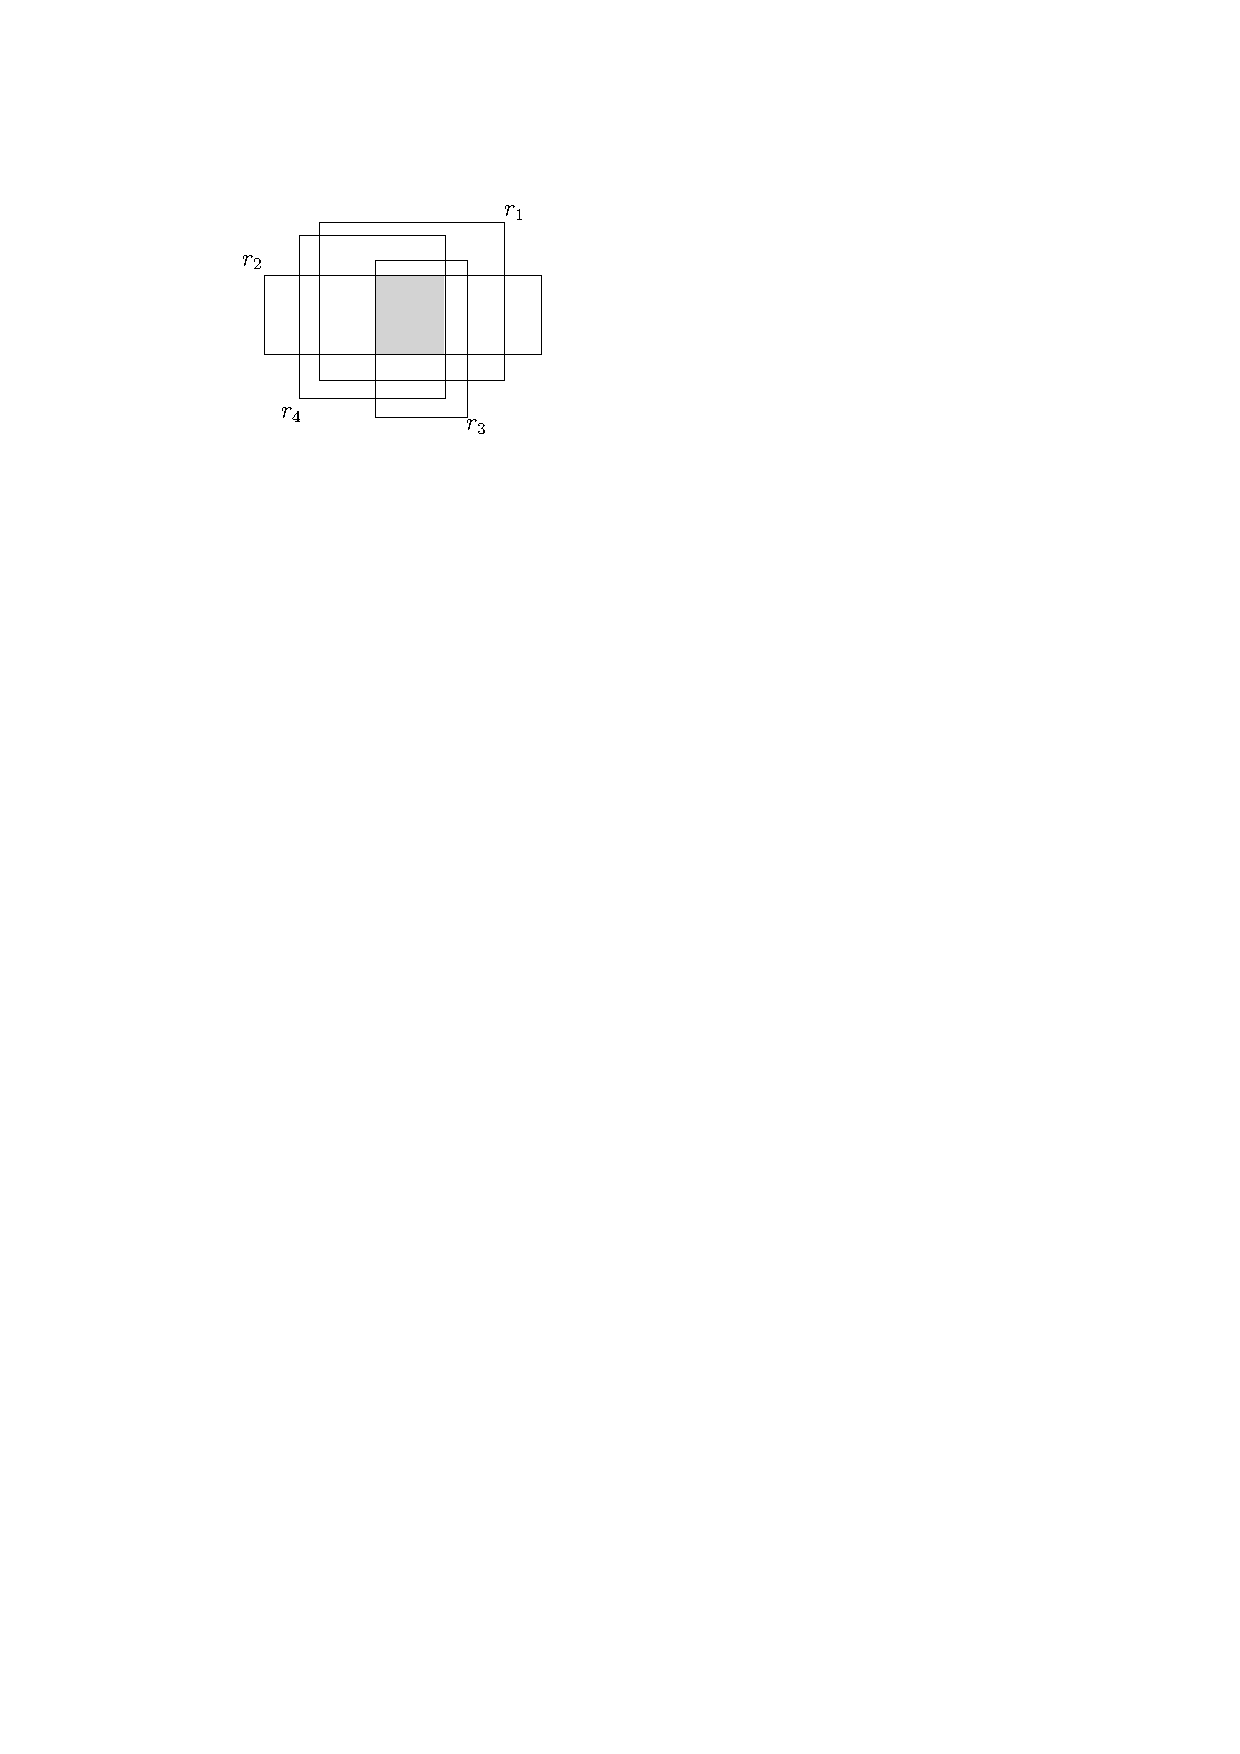
\includegraphics[height=27mm]{./artwork/guard}

    \figcapup
    \caption{Consider a 4-tuple $\bm{t} = \set{r_1, r_2, r_3, r_4}$. $B_\bm{t}$ is the rectangle in gray, $\gleft(\bm{t}) = r_3$ and $\gbot(\bm{t}) = r_2$.}
    \label{fig:guard}
    \figcapdown
\end{figure}


\begin{figure*}
    \begin{tabular}{ccccc}
        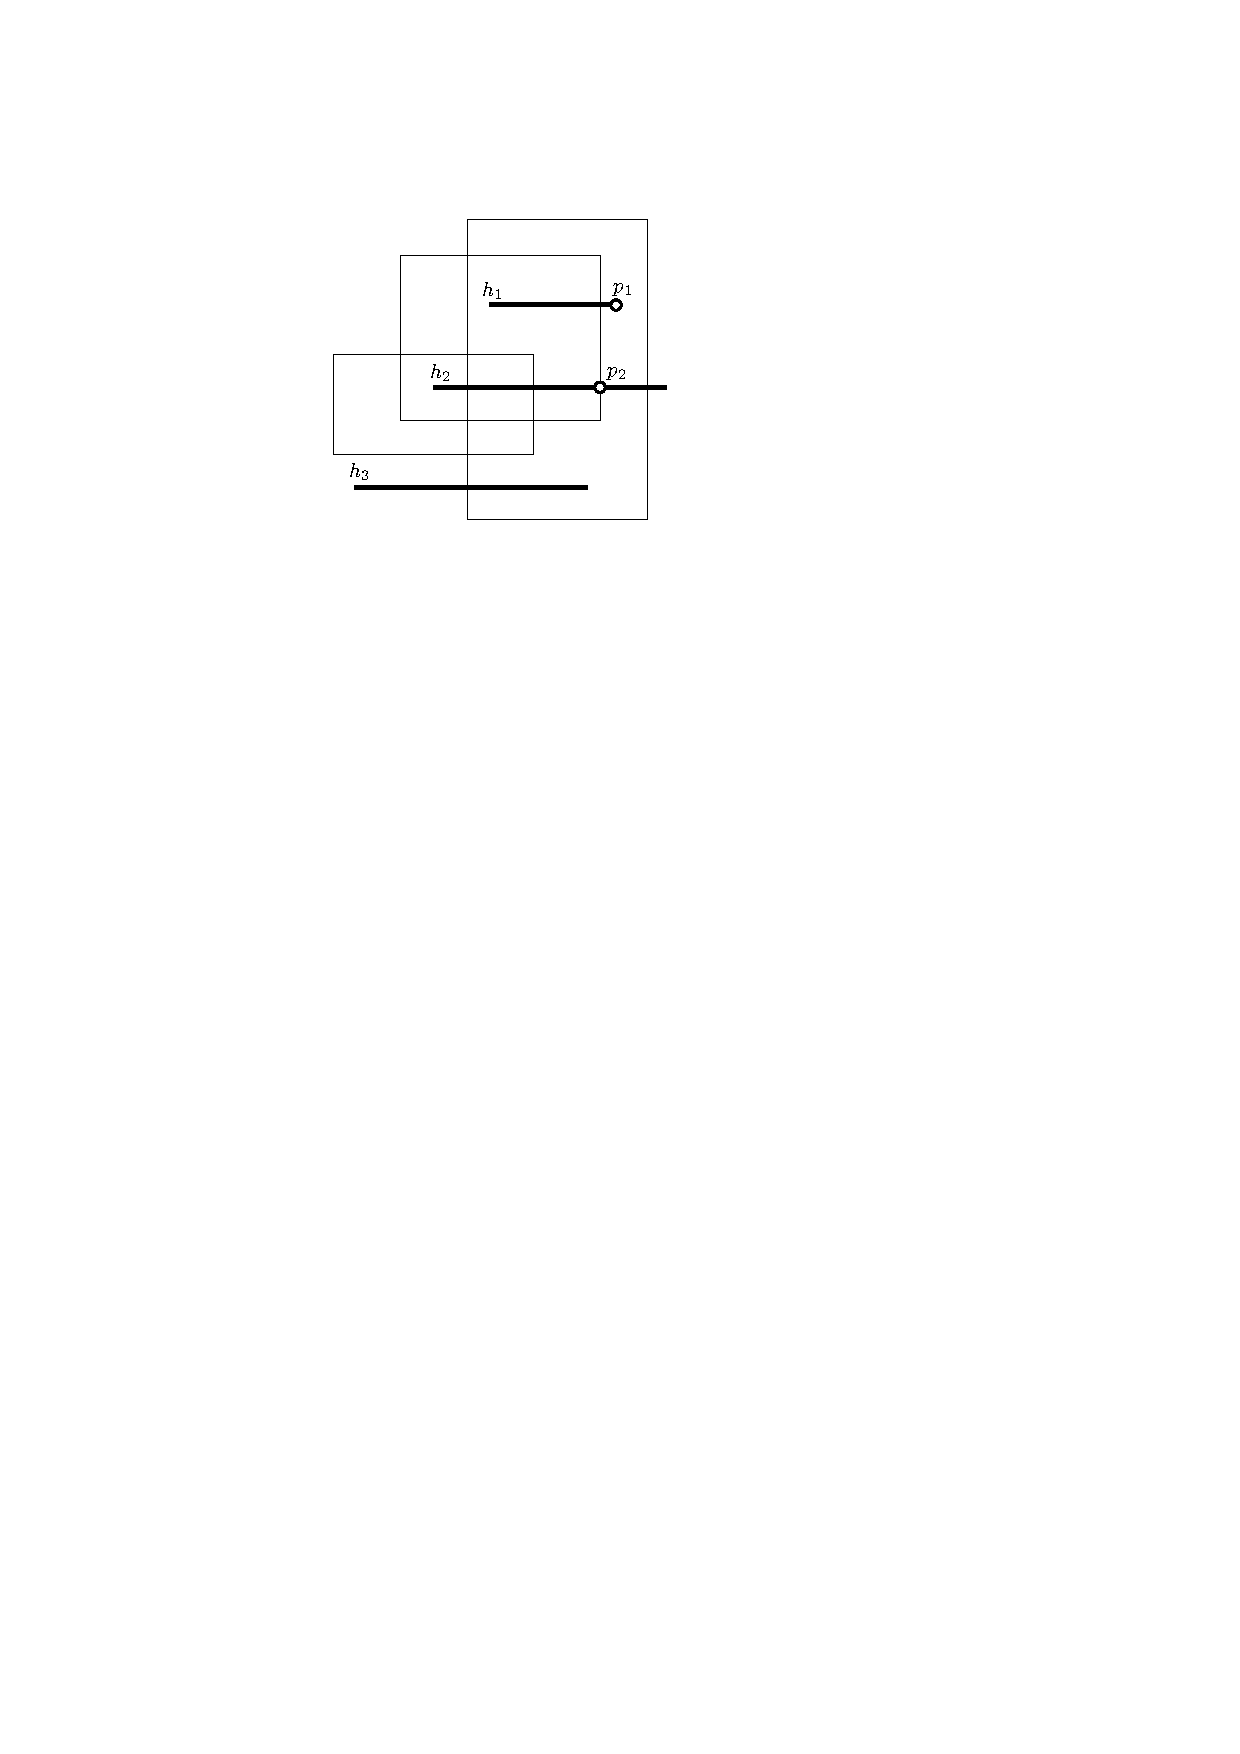
\includegraphics[height=30mm]{./artwork/prob-a} & 
        \hspace{3mm}
        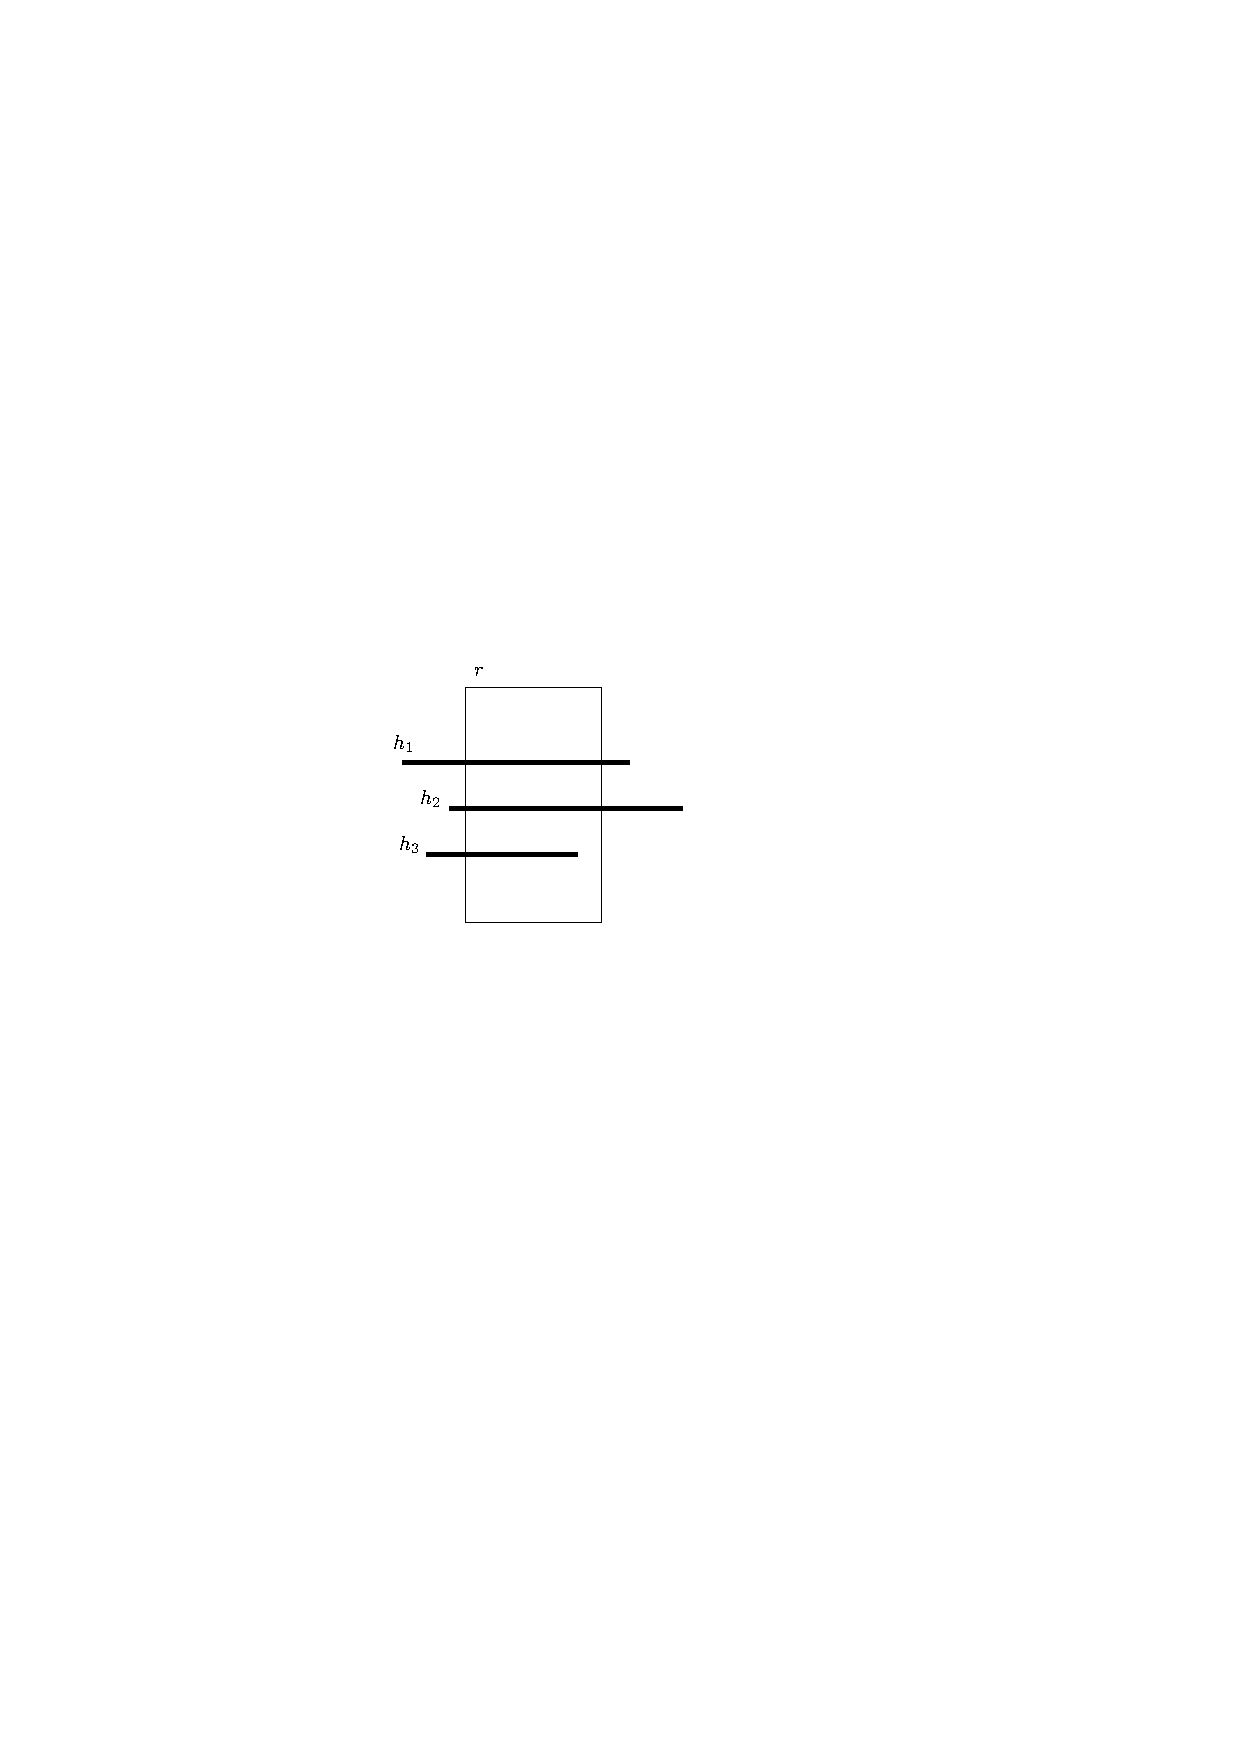
\includegraphics[height=27mm]{./artwork/prob-b} &
        \hspace{3mm}
        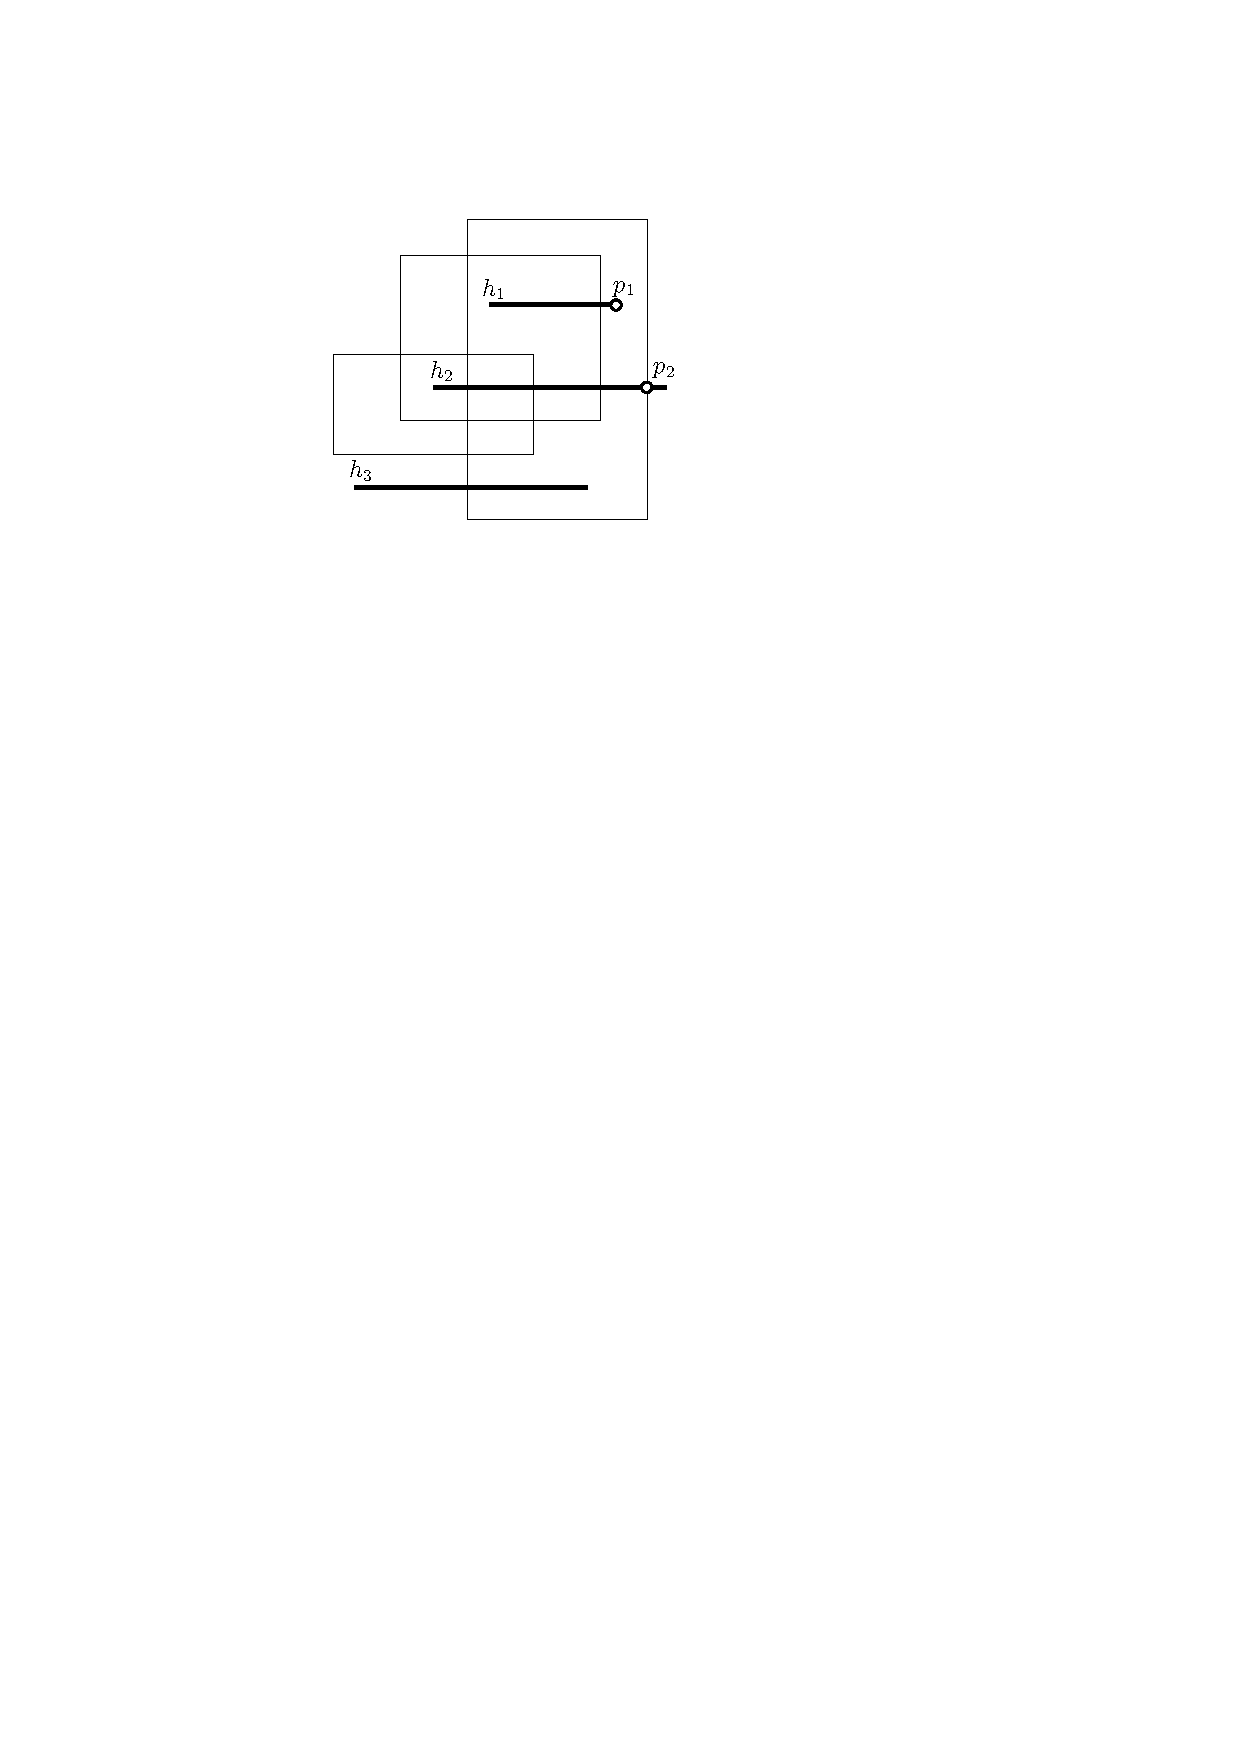
\includegraphics[height=30mm]{./artwork/prob-c} &
        \hspace{3mm}
        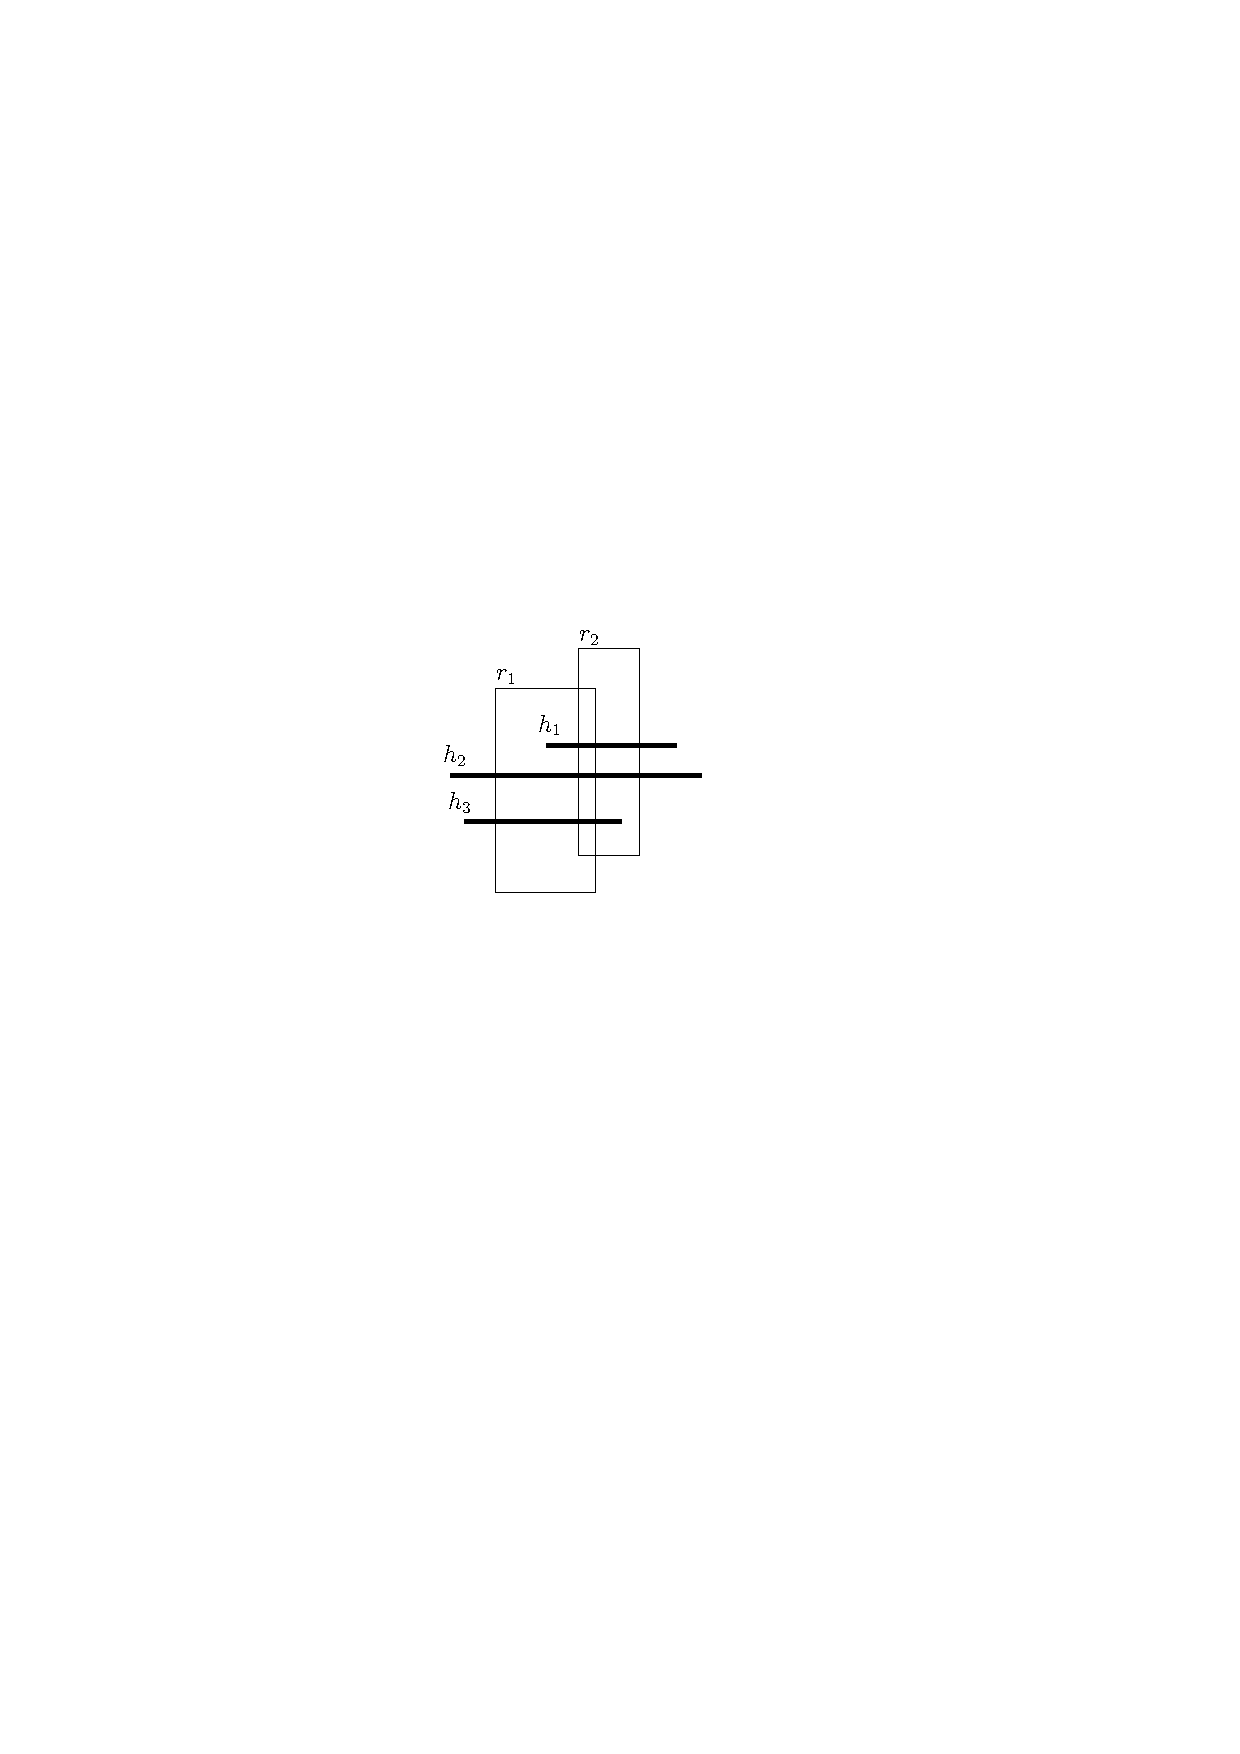
\includegraphics[height=30mm]{./artwork/prob-d} &
        \hspace{3mm}
        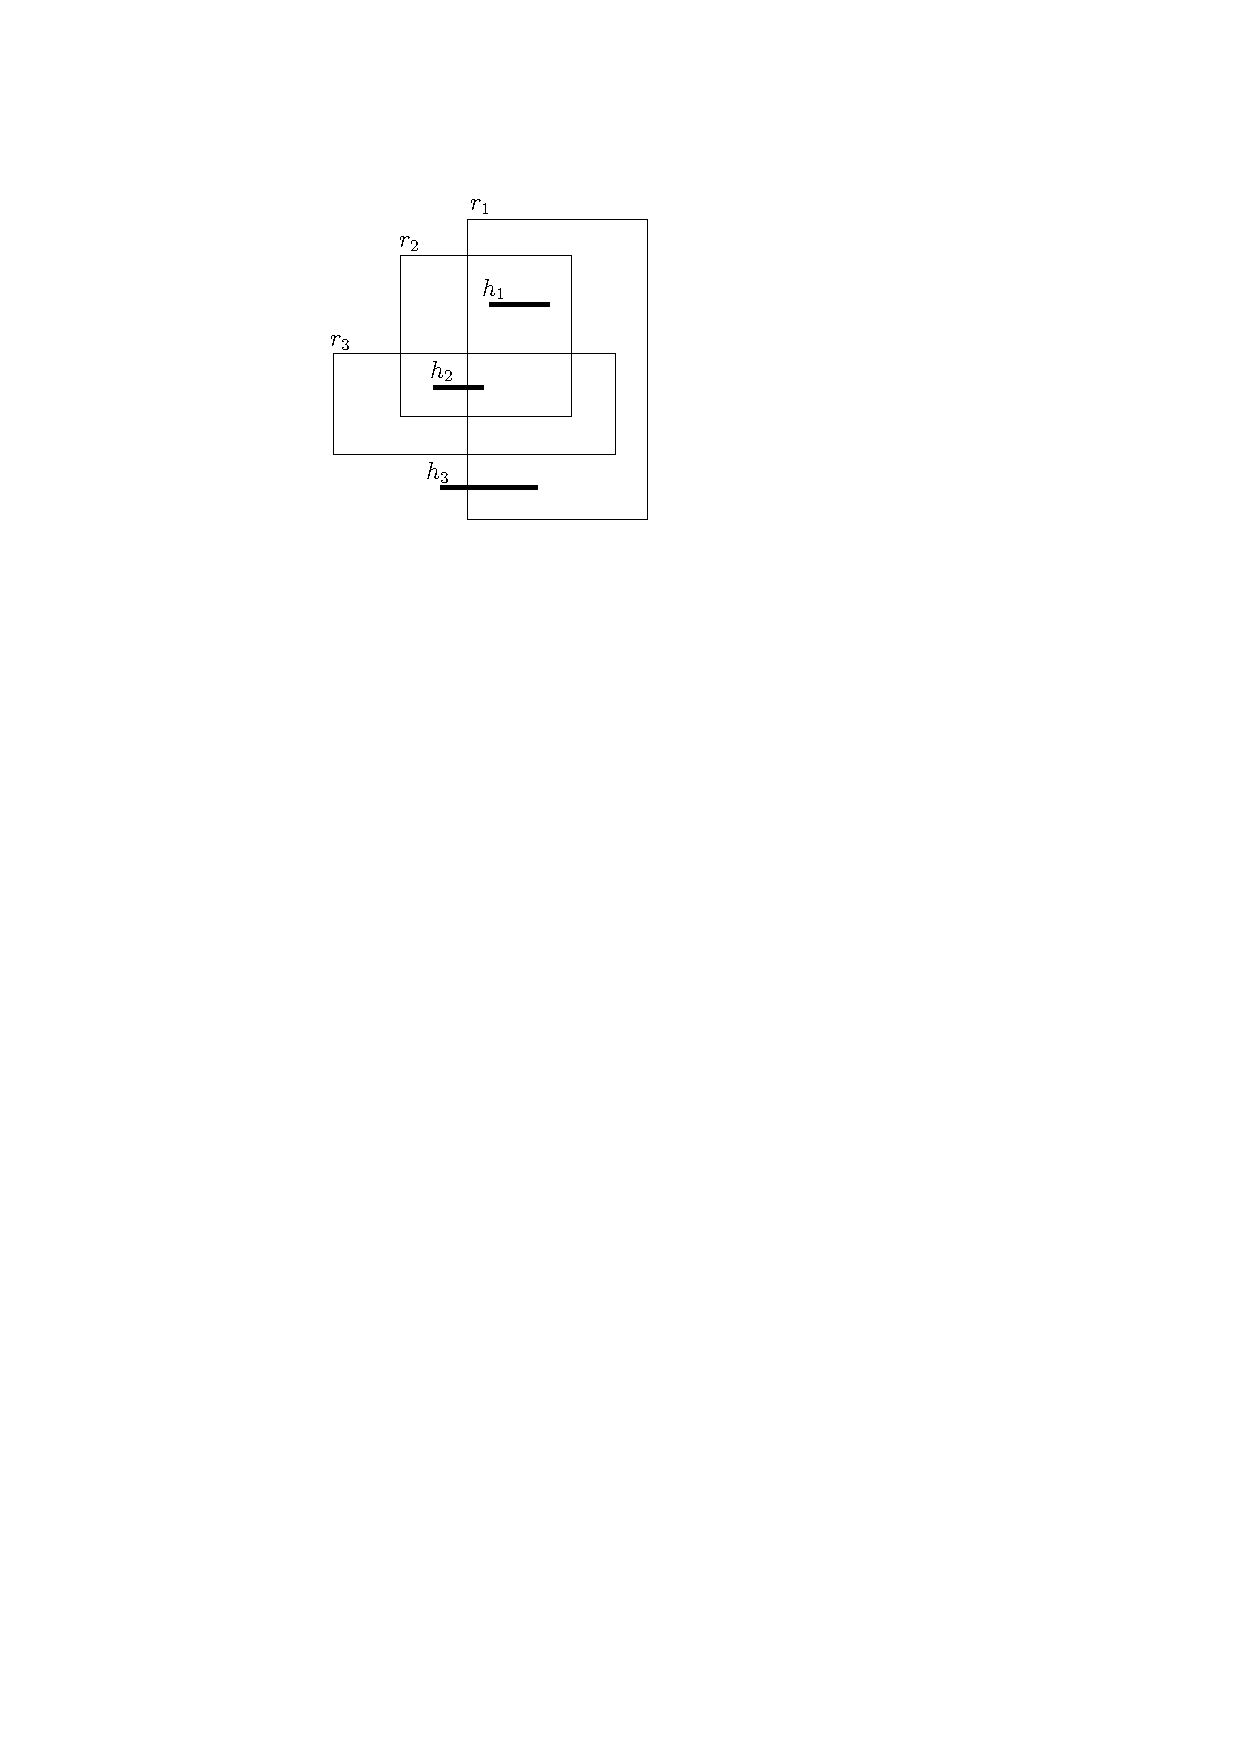
\includegraphics[height=30mm]{./artwork/prob-e} \\[2mm]
        (a) Problems $\mathscr{A}$ &
        \hspace{3mm}
        (b) Problem $\mathscr{B}$ &
        \hspace{3mm}
        (c) Problem $\mathscr{C}$ &
        \hspace{3mm}
        (d) Problem $\mathscr{D}$ &
        \hspace{3mm}
        (e) Problem $\mathscr{E}$
    \end{tabular}

    \figcapup
    \caption{Four geometric building brick problems}
    \label{fig:probs}
    \figcapdown
\end{figure*}

\section{Preliminaries in Geometry} \label{sec:bricks}

This section will first define some notions frequently used in our presentation and then introduce several  geometry problems, whose solutions will serve as building bricks for our $k$-SJ algorithm.

\extraspacing {\bf Terminology.} A {\em horizontal} segment is a segment of the form $[x_1, x_2] \times y$, and a {\em vertical} segment is a segment of the form $x \times [y_1, y_2]$. We say that a horizontal segment $h_1$ is {\em lower} (resp., {\em higher}) than another horizontal segment $h_2$ if the y-coordinate of $h_1$ is smaller (resp., larger) than that of $h_2$. Similarly, a vertical segment $v_1$ is {\em to the left} (resp., {\em right}) {\em of} another vertical segment $v_2$ if the x-coordinate of $v_1$ is smaller (resp., larger) than that of $v_2$.

\vgap

%Similarly, given a vertical segment $v$, we call a rectangle $r$ a {\em bottom-end covering rectangle} of $v$, if $r$ contains the bottom endpoint of $v$. \yf{need this?}

Given a horizontal segment $h = [x_1, x_2] \times y$, we call a rectangle $r$ a {\em left-end covering rectangle} of $h$, if $r$ contains the left endpoint of $h$ (i.e., $(x_1, y) \in r$). A horizontal/vertical segment $s$ {\em crosses} a rectangle $r$, if $s \cap r \ne \emptyset$ but $r$ covers neither of the two endpoints of $s$. A rectangle $r$ {\em contains} a horizontal/vertical segment $s$, if $r$ covers both endpoints of $s$.

\vgap

Let $S$ be a set of segments where either all segments are horizontal or all are vertical. Given a rectangle $r$, we define 
\myeqn{
    \cross_S(r) = \{s \in S \mid \text{$s$ crosses $r$} \}
    \label{eqn:cross}
}
namely, the set of segments in $S$ crossing $r$.
Let $R$ be a set of rectangles. Given a horizontal segment, we define 
\myeqn{
    \contained_R(h) = \{r \in R \mid \text{$h$ is contained in $r$} \}
    \label{eqn:contained}
}
namely, the set of rectangles in $R$ containing $h$.

\vgap

Given a rectangle $r = [x_1, x_2] \times [y_1, y_2]$, we define $\xleft(r) = x_1$, $\xright(r) = x_2$, $\ybot(r) = y_1$, and $\ytop(r) = y_2$. Consider a $k$-tuple $\bm{t} = (r_1, r_2, ..., r_k)$ where $k \ge 2$, and each $\bm{t}[i] = r_i$ ($i \le [k]$) is a rectangle. We define 
\myeqn{
    B_\bm{t} &=& \cap_{i=1}^t r_i \label{eqn:B_t}
}
namely, $B_\bm{t}$ is the intersection of the rectangles in $\bm{t}$ (note: $B_\bm{t}$ is a rectangle itself). Also, define:
\myitems{
    \item $\gleft(\bm{t})$ as the rectangle $r_i$, $i \in [k]$, satisfying $\xleft(r_i)$ $= \xleft(B_\bm{t})$. In case multiple values in $[k]$ fulfill the condition, let $i$ be the smallest of such values.

    \item $\gbot(\bm{t})$ as the rectangle $r_i$, $i \in [k]$, satisfying $\ybot(r_i)$ $= \ybot(B_\bm{t})$. In case multiple values in $[k]$ fulfill the condition, let $i$ be the smallest of such values.
}
See Figure~\ref{fig:guard} for an illustration. It is worth mentioning that since a horizontal segment $h$ is a degenerated rectangle, notations such as $\xleft(h)$ and $\xright(h)$ are well-defined.

\extraspacing {\bf Problem $\bm{\mathscr{A}}$.} The input involves a set $P$ of 2D points and set $R$ of rectangles. In the {\em detection version} of Problem $\mathscr{A}$, the goal is to output, for each point $p \in P$, whether it is covered by at least one rectangle in $R$. Figure~\ref{fig:probs}a gives an example where $P = \set{p_1, p_2, p_3}$ and $R = \set{r_1, r_2}$; the output is ``yes'' for $p_2$ and $p_3$ and ``no'' for $p_1$. This can be achieved in $O(n \log n)$ time where $n = |P| + |R|$ as shown
in Appendix~\ref{app:bricks}.

\vgap

In the {\em reporting version} of Problem $\mathscr{A}$, the goal is to output, for each point $p \in P$, all the rectangles $r \in R$ containing $p$. In Figure~\ref{fig:guard}a, for instance, the output is $\set{(p_1, \emptyset), (p_2: r_1, r_2), (p_3: r_2)}$. As shown in Appendix~\ref{app:bricks}, this can be achieved in $O(n \log n + \out)$ time, where $\out$ is the number of pairs $(p, r) \in P \times R$ such that $p \in r$.

\extraspacing {\bf Problem $\bm{\mathscr{B}}$.} The input involves a set $H$ of horizontal segments and a set $V$ of vertical segments. The goal is to report, for each segment $h \in H$, the leftmost point $p$ on $h$ such that $p$ is on some vertical segment in $V$. If $h$ does not intersect with any segment in $V$, report nothing for $h$. Figure~\ref{fig:probs}b gives an example where $H = \set{h_1, h_2, h_3}$ and $V = \set{v_1, v_2}$; the output is $\set{(h_1, p_1), (h_2, p_2)}$. This problem can be solved in $O(n \log n)$ time where $n = |H| + |V|$, as shown in Appendix~\ref{app:bricks}.


\extraspacing {\bf Problem $\bm{\mathscr{C}}$.} The input involves a set $H$ of horizontal segments and a set $R$ of rectangles. The goal is to report, for each segment $h \in H$, the rightmost point $p$ on $h$ such that $p$ is covered by at least one left-end covering rectangle of $h$ in $R$ --- formally, for $h = [x_1, x_2] \times y$, we aim to find the maximum $x \in [x_1, x_2]$ such that at least one rectangle $r \in R$ covers both the point $(x_1, y)$ and the point $(x, y)$. If the point $p$ exists (i.e., $h$ has at least one left-end covering rectangle in $R$), we should output a tuple $(h, p)$; otherwise, output nothing for $h$. Figure~\ref{fig:probs}c gives an example where $H = \set{h_1, h_2}$ and $R$ includes the three rectangles shown; the output is $\set{(h_1, p_1), (h_2, p_2)}$. This problem can be solved in in $O(n \log n)$ time where $n = |H| + |R|$, as shown in Appendix~\ref{app:bricks}.

\extraspacing {\bf Problem $\bm{\mathscr{D}}$.} The input involves a set $H$ of horizontal segments and a set $R$ of rectangles. In the {\em find-lowest} version of the problem, the goal is to report, for each rectangle $r \in R$, the lowest segment in $\cross_H(r)$ (see its definition in \eqref{eqn:cross}). If no segment in $H$ crosses $r$, output nothing for $r$.  Figure~\ref{fig:probs}d gives an example where $H = \set{h_1, h_2, h_3}$ and $R = \set{r_1, r_2}$; the output is $\set{(r_1, h_3), (r_2, h_2)}$. This can be achieved in $O(n \log n)$ time where $n = |H| + |R|$, as shown in Appendix~\ref{app:bricks}.

\vgap

In the {\em find-all-sorted} version of the problem, the goal is to report, for each rectangle $r \in R$, the entire $\cross_H(r)$ sorted by y-coordinate. Formally, if $\cross_H(r) = \set{h_1, h_2, ..., h_z}$ for some $z \ge 1$, we output $(r: h_1, h_2, ..., h_z)$, provided that $y_i \ge y_{i-1}$ for each $i \in [2, z]$ where $y_i$ (resp., $y_{i-1}$) is the y-coordinate of $h_i$ (resp., $h_{i-1}$). In the example of Figure~\ref{fig:probs}d, the output is $\set{(r_1: h_3, h_2), (r_2: h_2, h_1)}$. In Appendix~\ref{app:bricks}, we explain how to solve the problem in $O(n \log n + \out)$ time where $\out$ is the number of pairs $(h, r) \in H \times R$ such that $h$ crosses $r$.


\extraspacing {\bf Problem $\bm{\mathscr{E}}$.} The input involves a set $H$ of horizontal segments and a set $R$ of rectangles. The goal is to report, for each segment $h \in H$, the set $\contained_R(h)$ --- defined in \eqref{eqn:contained} --- where the rectangles are sorted by their right boundaries. Formally, if $r_1, r_2, ..., r_z$ for some $z \ge 1$ are all the rectangles in $\contained_R(h)$, we output $(h: r_1, r_2, ..., r_z)$, provided that $\xright(r_i) \ge \xright(r_{i-1})$ for each $i \in [2, z]$. Figure~\ref{fig:probs}e gives an example where $H = \set{h_1, h_2, h_3}$ and $R = \set{r_1, r_2, r_3}$; the output is $\set{(h_1: r_2, r_1), (h_2: r_2, r_3), (h_3: \emptyset)}$. In Appendix~\ref{app:bricks}, we explain how to solve the problem in $O(n \log n + \out)$ time where $n = |H| + |R|$ and $\out$ is the number of pairs $(h, r) \in H \times R$ such that $r$ contains $h$.


\section{The Core: H-V Multiway Spatial Joins} \label{sec:hv}

Recall that the input of $k$-SJ comprises $k$ sets of rectangles: $R_1, R_2, ...,$ $R_k$. We now formulate a special version of $k$-SJ, named the {\em H-V $k$-SJ problem}. The special nature is reflected in the introduction of three constraints: (i) $k \ge 3$, (ii) $R_{k-1}$ should be a set of horizontal segments, and (iii) $R_k$ should be a set of vertical segments. For better clarity, we will represent the input sets as $R_1, R_2, ..., R_{k-2}, H$ ($=R_{k-1}$), and $V$ ($=R_k$). The goal is to output the join result $\J(R_1, ..., R_{k-2},$ $H, V)$, including every $k$-tuple $(r_1, ..., r_{k-2}, h, v) \in R_1 \times ... \times R_{k-2} \times H \times V$ such that $h \cap v \cap \bigcap_{i=1}^{k-2} r_i$ is not empty.

\vgap

Our objective is to prove that H-V $k$-SJ can be efficiently reduced to $(k-1)$-SJ --- note: it is $(k-1)$-SJ here, rather than H-V $(k-1)$-SJ. To ensure the soundness of our notation system, let us formulate the ``1-SJ'' as the trivial problem where the input is a set $R$ of $n$ rectangles, and the goal is simply to enumerate each rectangle of $R$; the problem can obviously be ``solved'' in $O(n)$ time. We assume the existence of an algorithm $\A$ that can settle $\kappa$-SJ for all $\kappa \in [1, k-1]$. Denote by $F_\kappa(n, \out)$ the worst-case runtime of $\A$ on any instance of $\kappa$-SJ that has input size $n$ and output size $\out$. We consider that $F_\kappa(n, \out) \le F_{\kappa + 1}(n, \out)$ for any $\kappa \ge 1$, that is, its overhead on $\kappa$-SJ should not be larger than that on $(\kappa+1)$-SJ.

\vgap

We will establish:

\begin{lemma} \label{lmm:hv}
    Equipped with the algorithm $\A$ described above, the H-V $k$-SJ problem can be solved in time
    \myeqn{
        O(k) \cdot \big( F_{k-1}(n, \out) + n\log n + k \cdot \out \big) \nn
    }
    where $n$ (resp., $\out$) is the input (resp., output) size of the problem. Furthermore, if $\A$ is comparison-based, so is the H-V $k$-SJ algorithm.
\end{lemma}

The part of the paper from this point till the end of Section~\ref{sec:hv:type2} will be devoted to proving the above lemma. This is the most challenging step in solving the general $k$-SJ problem optimally, as will be discussed in Section~\ref{sec:ksj}, where we will prove Theorems~\ref{thm:main-recur} and \ref{thm:main-alg} based on Lemma~\ref{lmm:hv}.

\vgap

%The condition is equivalent to saying that the intersection point of $h$ and $v$ falls in every $r_i$ of $i \in [k-2]$.


Consider any $k$-tuple $(r_1, ..., r_{k-2}, h, v)$ in the join result $\J(R_1, ...,$ $R_{k-2}, H, V)$. We classify the tuple into one of the two types below:

\myitems{
    \item {{\bf Type 1:}} $h$ crosses all of $r_1, ..., r_{k-2}$ and, at the same time, $v$ crosses all of $r_1, ..., r_{k-2}$; 
    
    \item {{\bf Type 2:}} either $h$ or $v$ fails to cross at least one rectangle in $\set{r_1, r_2, ..., r_{k-2}}$. Equivalently,
    there exists at least a rectangle $r_i$ (for some $i \in [k-2]$) that covers an endpoint of either $h$ or $v$ or both.
}
Figure~\ref{fig:hv:types} illustrates a result tuple of each type, assuming $k = 4$. In Section~\ref{sec:hv:type1} (resp., \ref{sec:hv:type2}), we will explain how to produce the result tuples of Type 1 (resp., 2) in the time complexity claimed in Lemma~\ref{lmm:hv}.

\extraspacing {\bf Remark.} In \cite{rdr+11}, Rahul et al.\ studied the problem of storing a set $H$ of horizontal segments and a set $V$ of vertical segments in a data structure such that, given a query rectangle $r$, all the pairs $(h, v) \in H \times V$ satisfying $h \cap v \cap r \ne \emptyset$ can be reported efficiently. They developed a structure of $O(n \log n)$ space that can be built in $O(n \log n)$ time, and can be used to answer a query in $O(\log n + K)$ time, where $n = |H| + |V|$ and $K$ is the number of pairs reported. Their structure can be utilized to solve H-V 3-SJ in $O(n \log n + \out)$ time. We are unaware of a way to extend their solution to handle H-V $k$-SJ of $k > 3$. Our method for proving Lemma~\ref{lmm:hv} is based on fundamentally different ideas even for $k = 3$.

\begin{figure}
    \begin{tabular}{cc}
        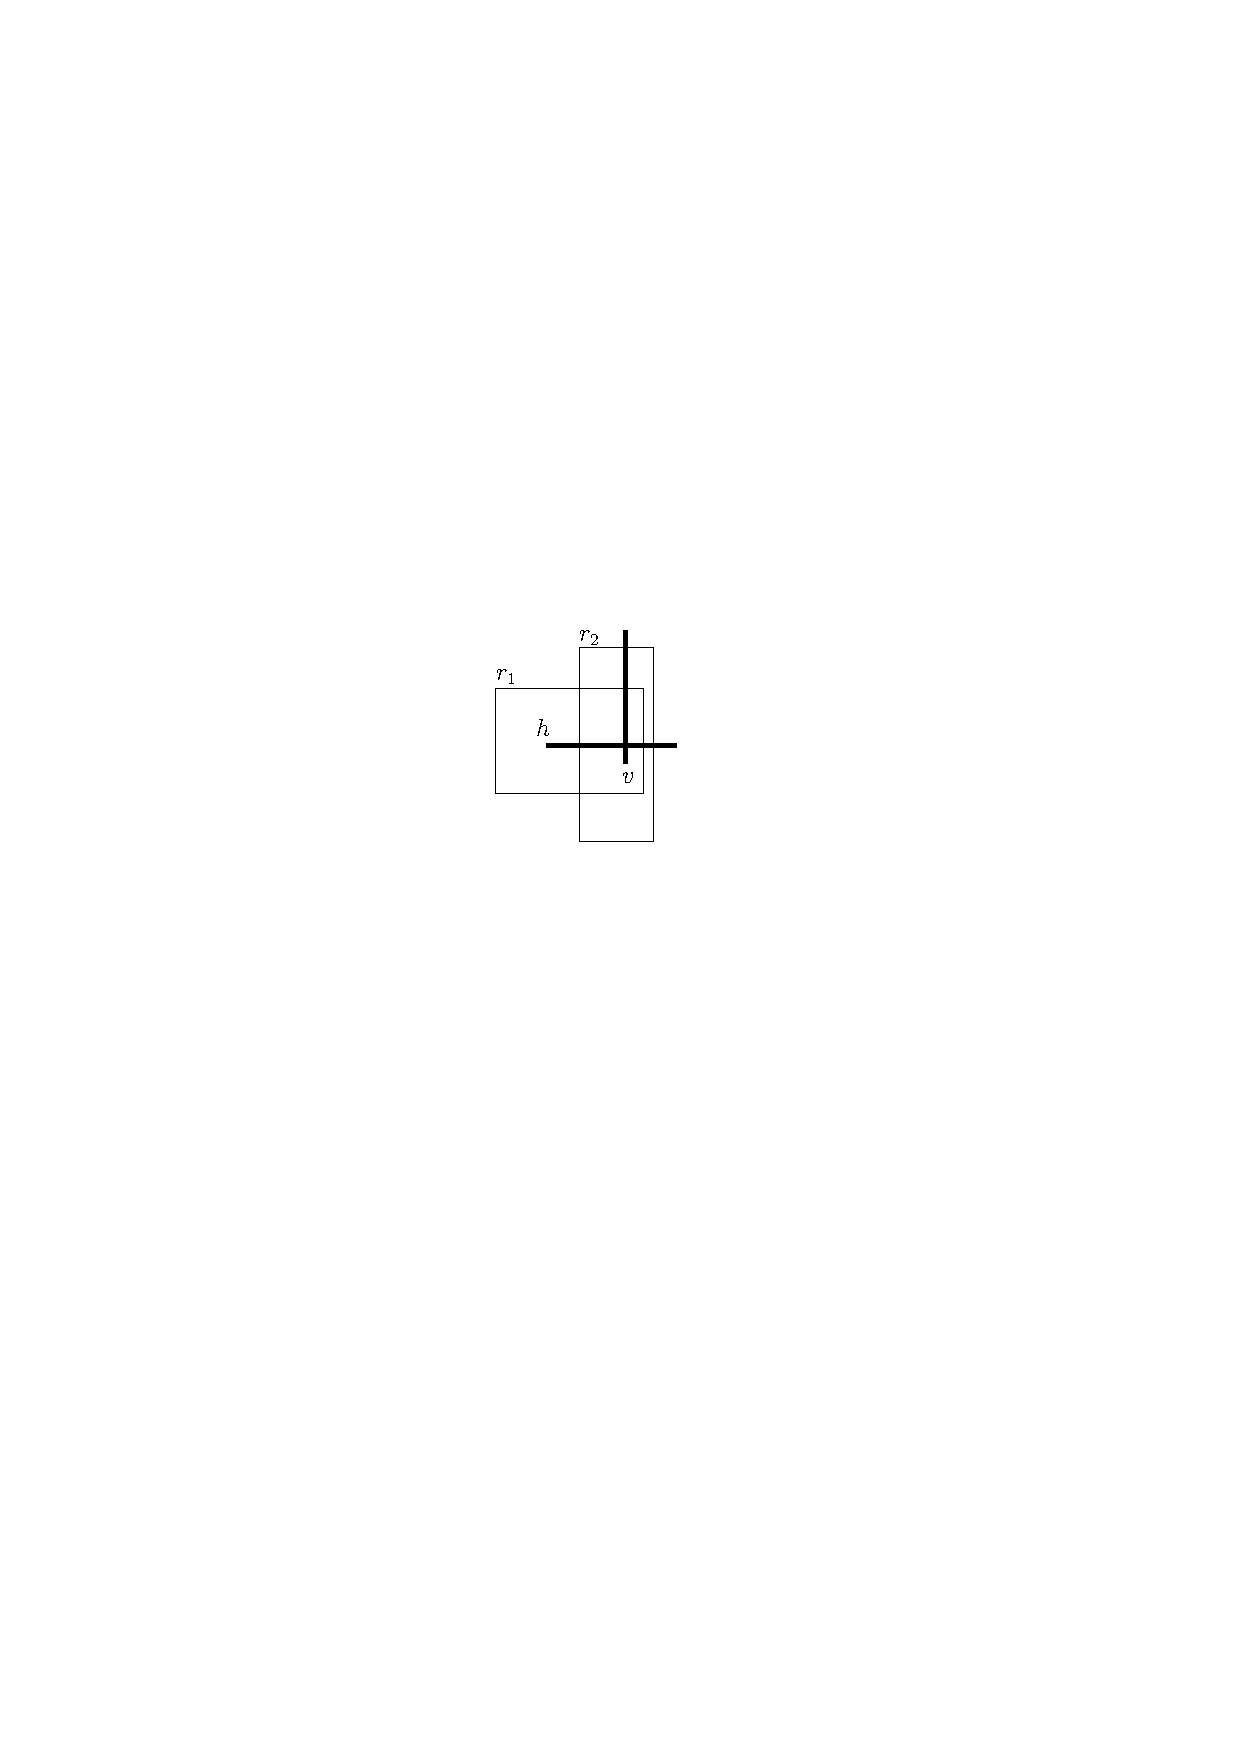
\includegraphics[height=27mm]{./artwork/type1} &
        \hspace{5mm} 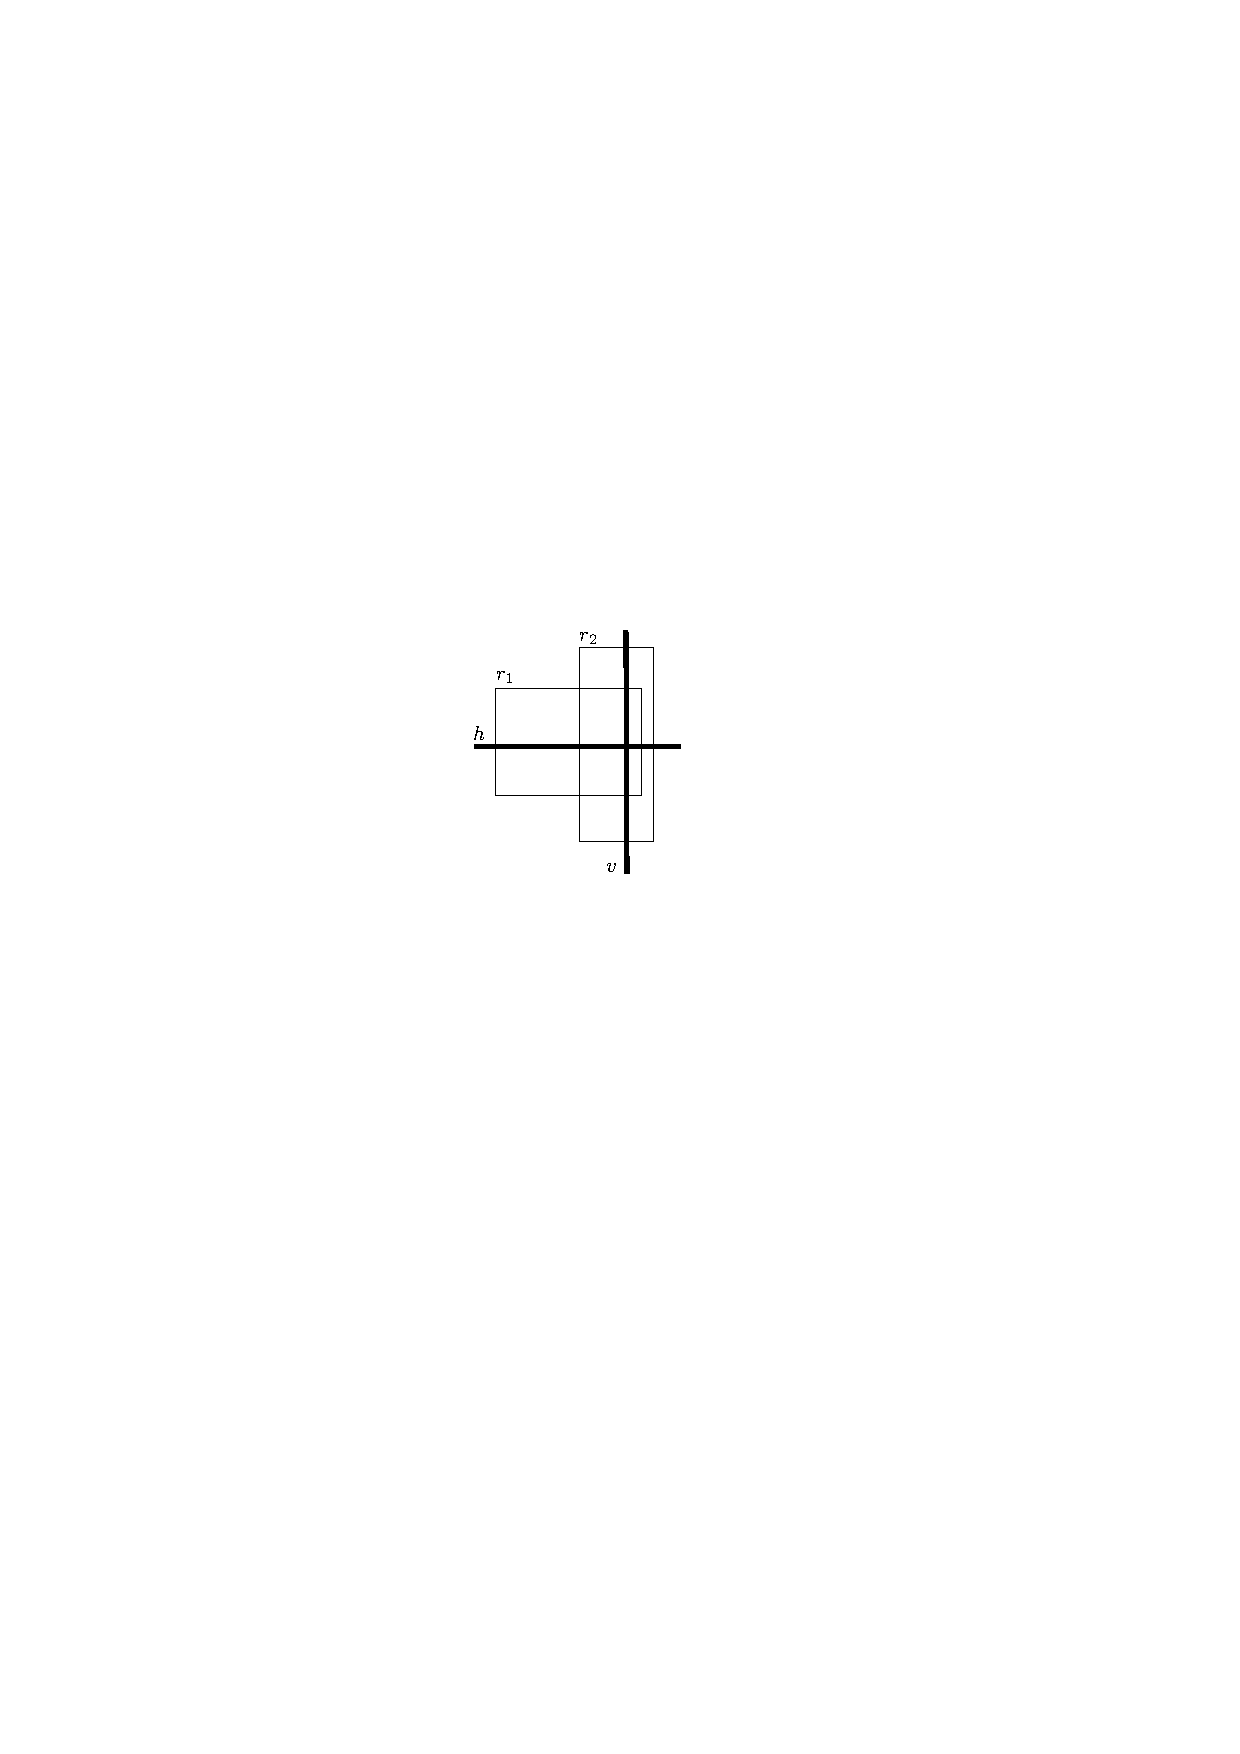
\includegraphics[height=23mm]{./artwork/type2} \\
        (a) Type 1 &
        (b) Type 2
    \end{tabular}

    \figcapup
    \caption{Classifying H-V $k$-SJ result tuples ($k$ = 4)}
    \label{fig:hv:types}
    \figcapdown
\end{figure}


\begin{figure*}
    \begin{tabular}{cccc}
        \hspace{-5mm}
        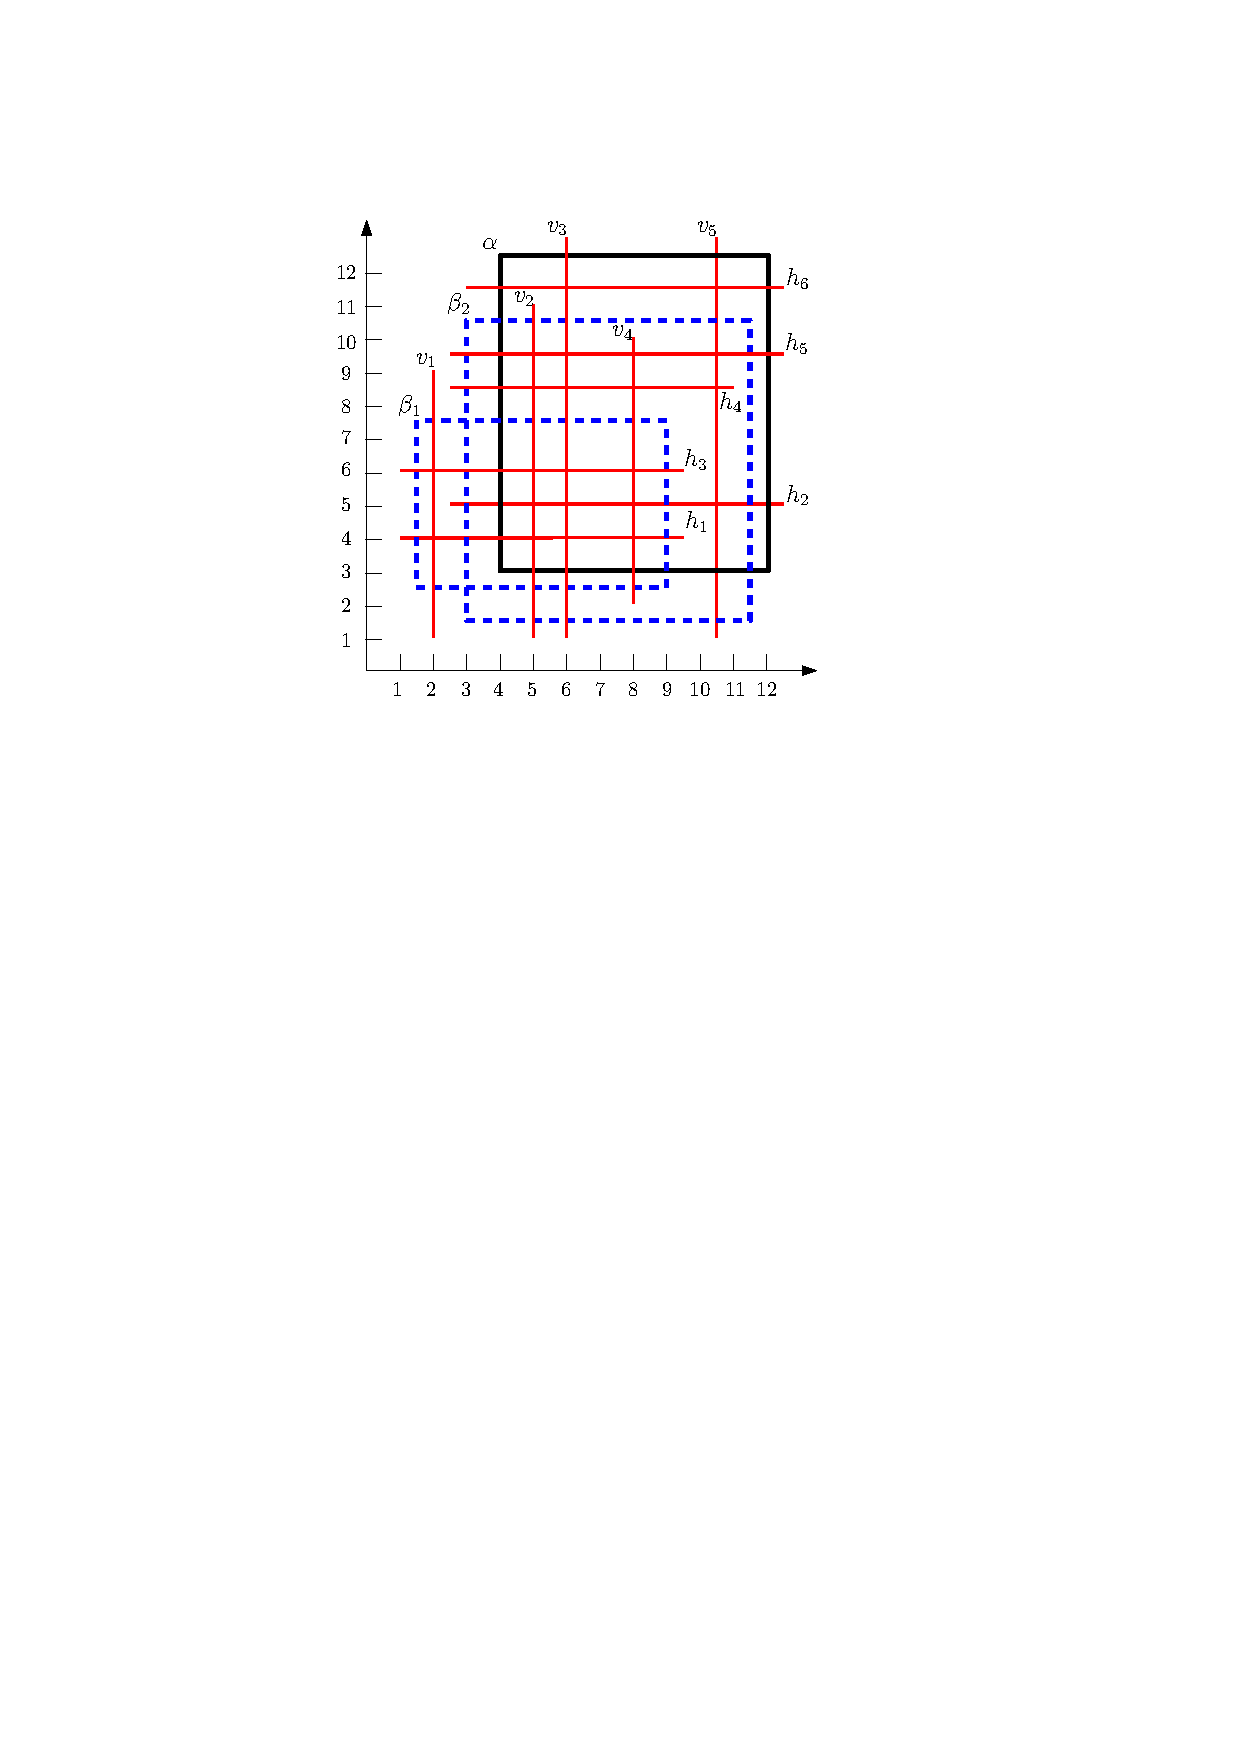
\includegraphics[height=45mm]{./artwork/alg-ex1-a} &
        \hspace{-4mm}
        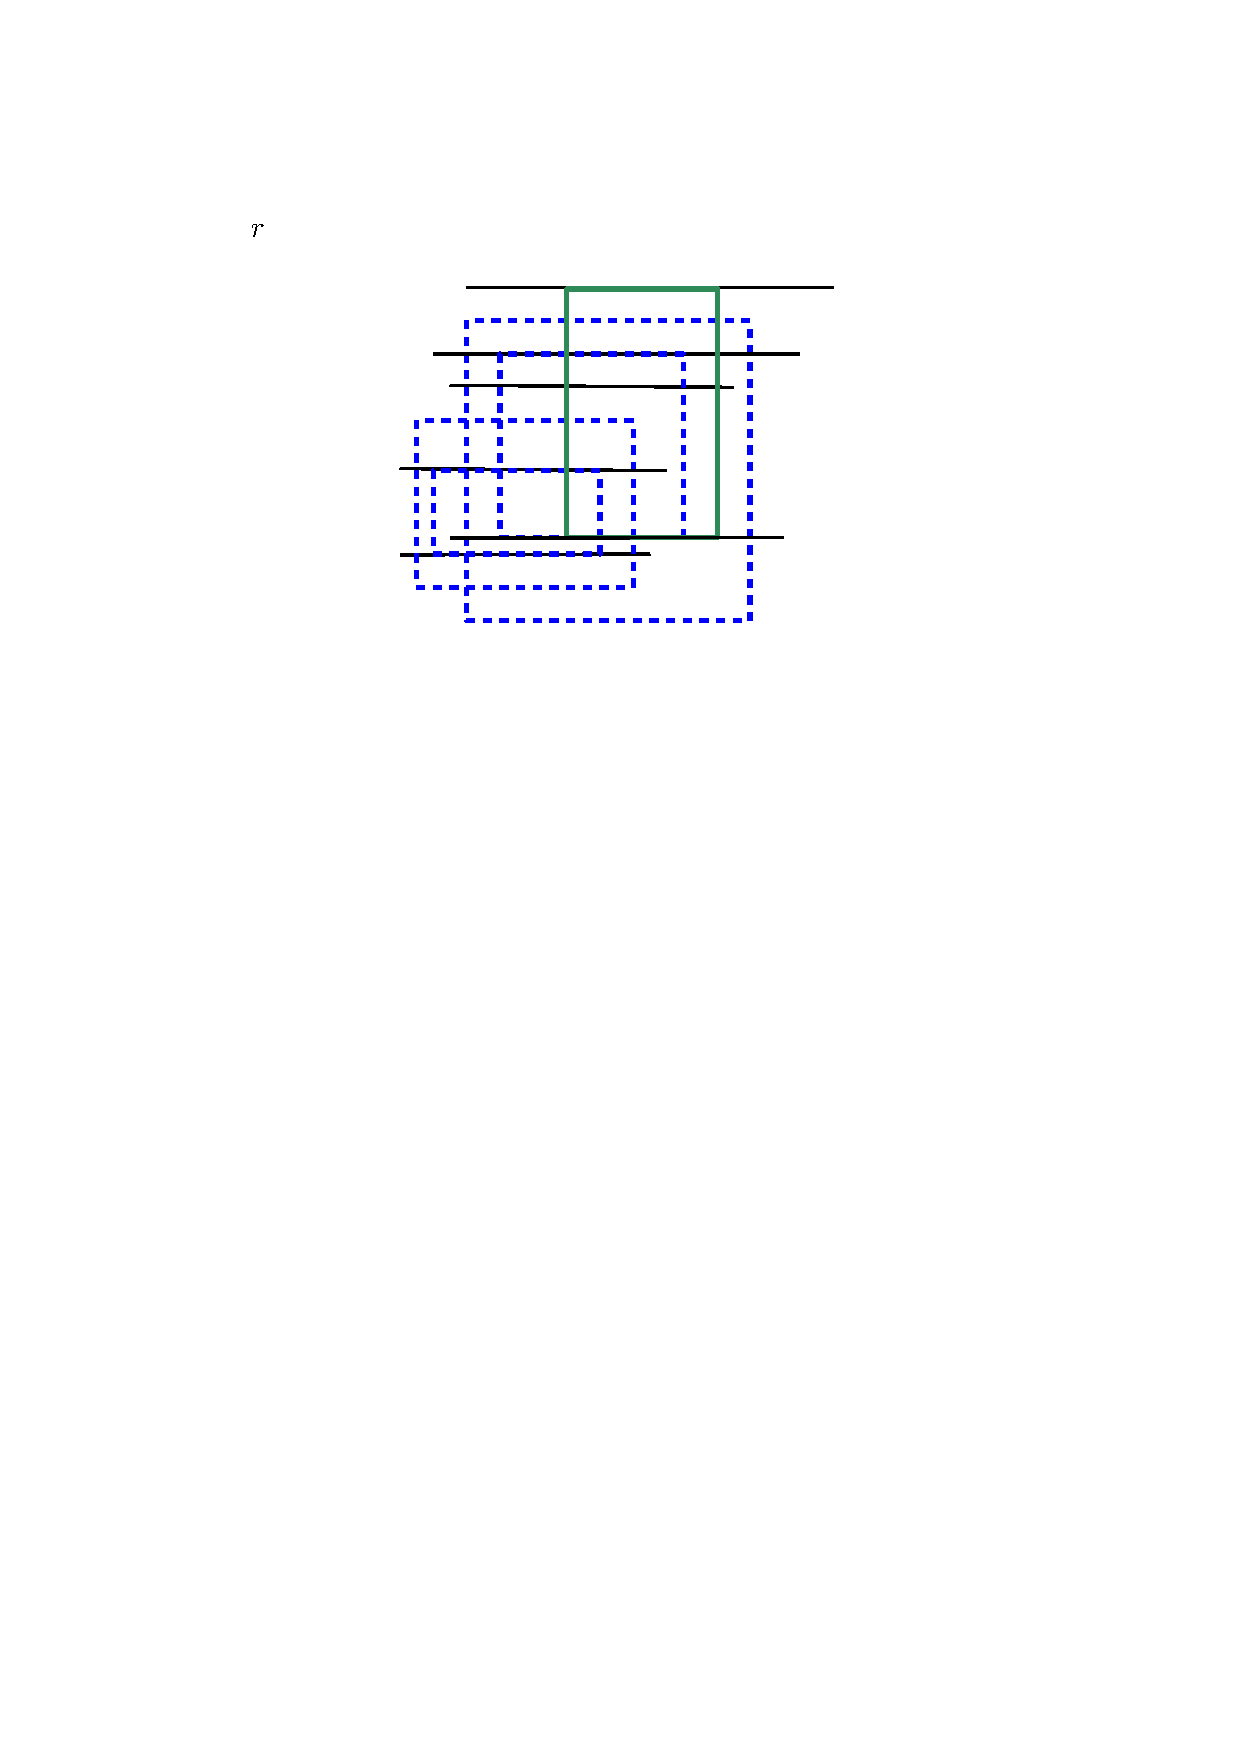
\includegraphics[height=45mm]{./artwork/alg-ex1-b} & 
        \hspace{-4mm}
        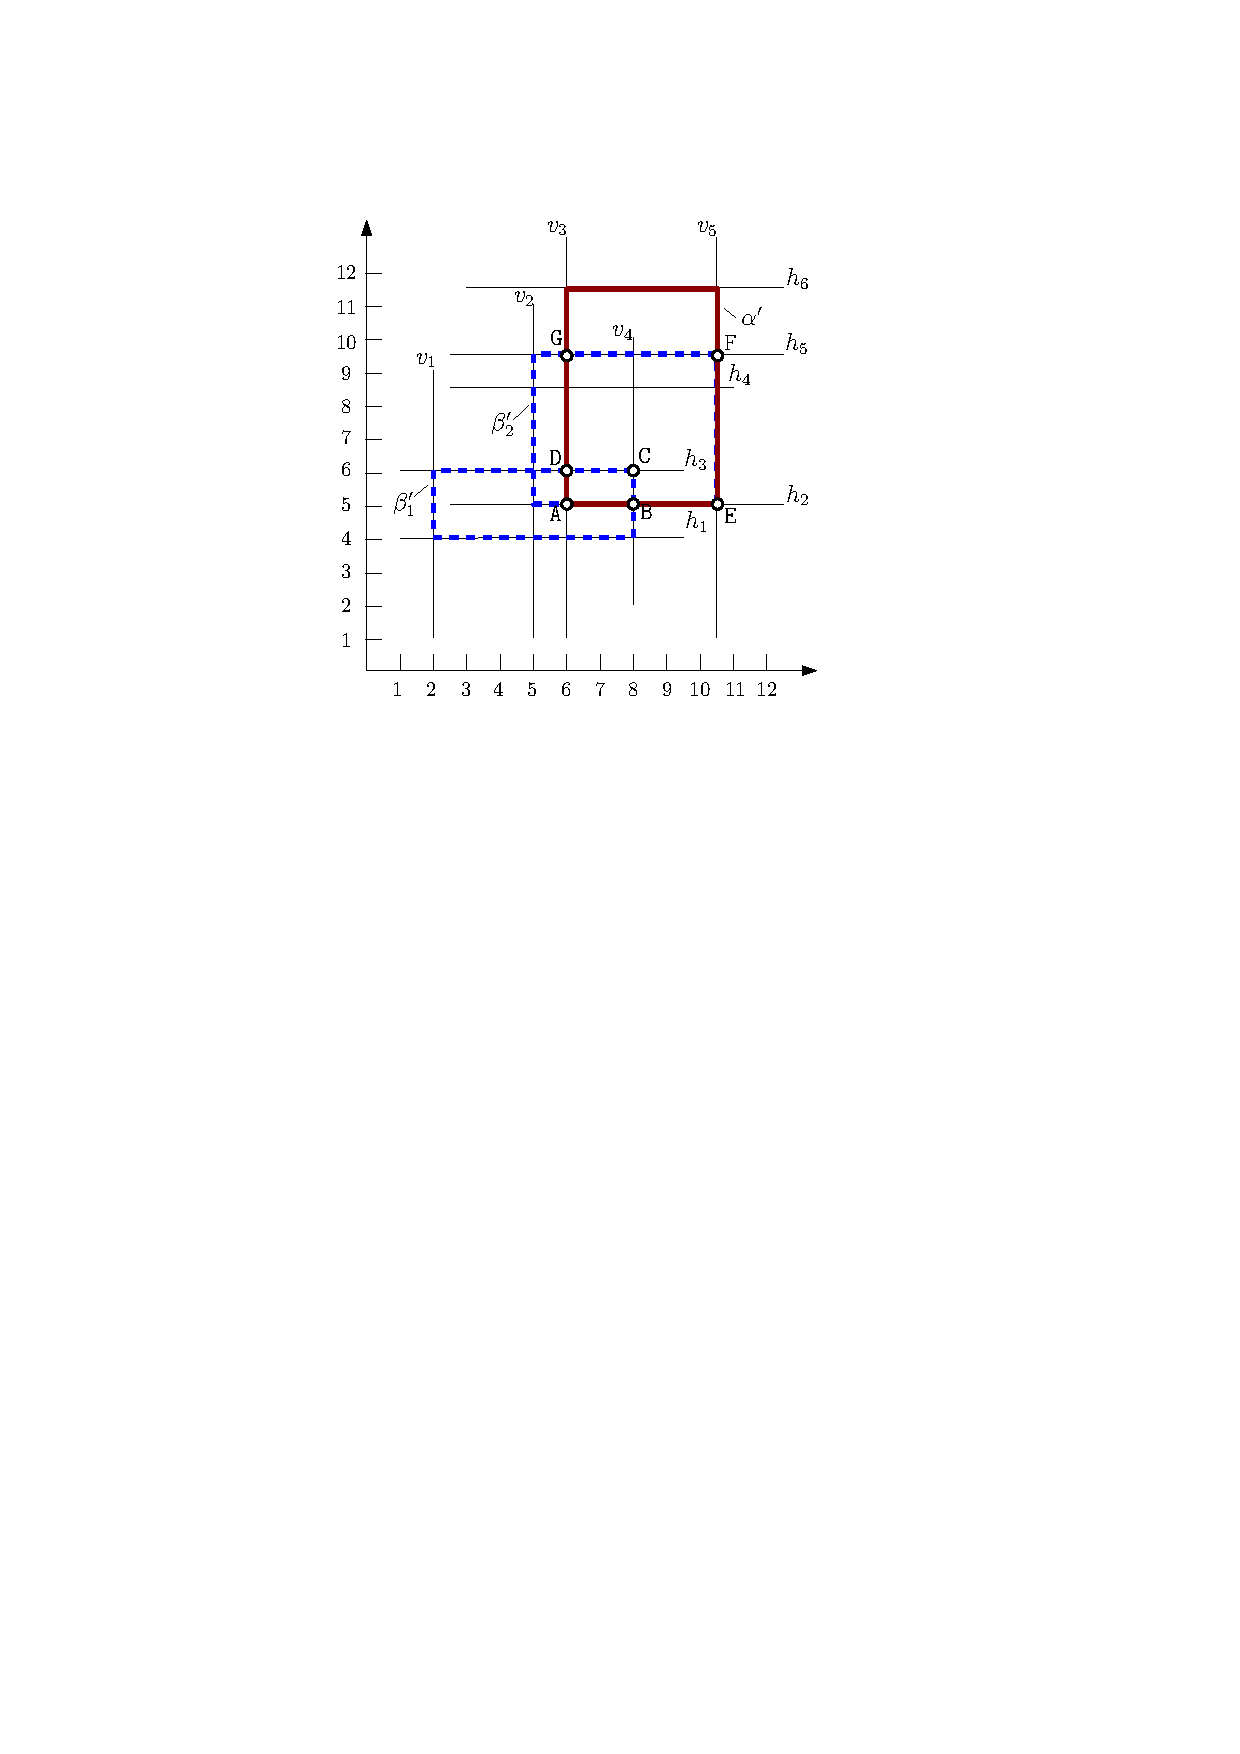
\includegraphics[height=45mm]{./artwork/alg-ex1-c} &
        \hspace{-4mm}
        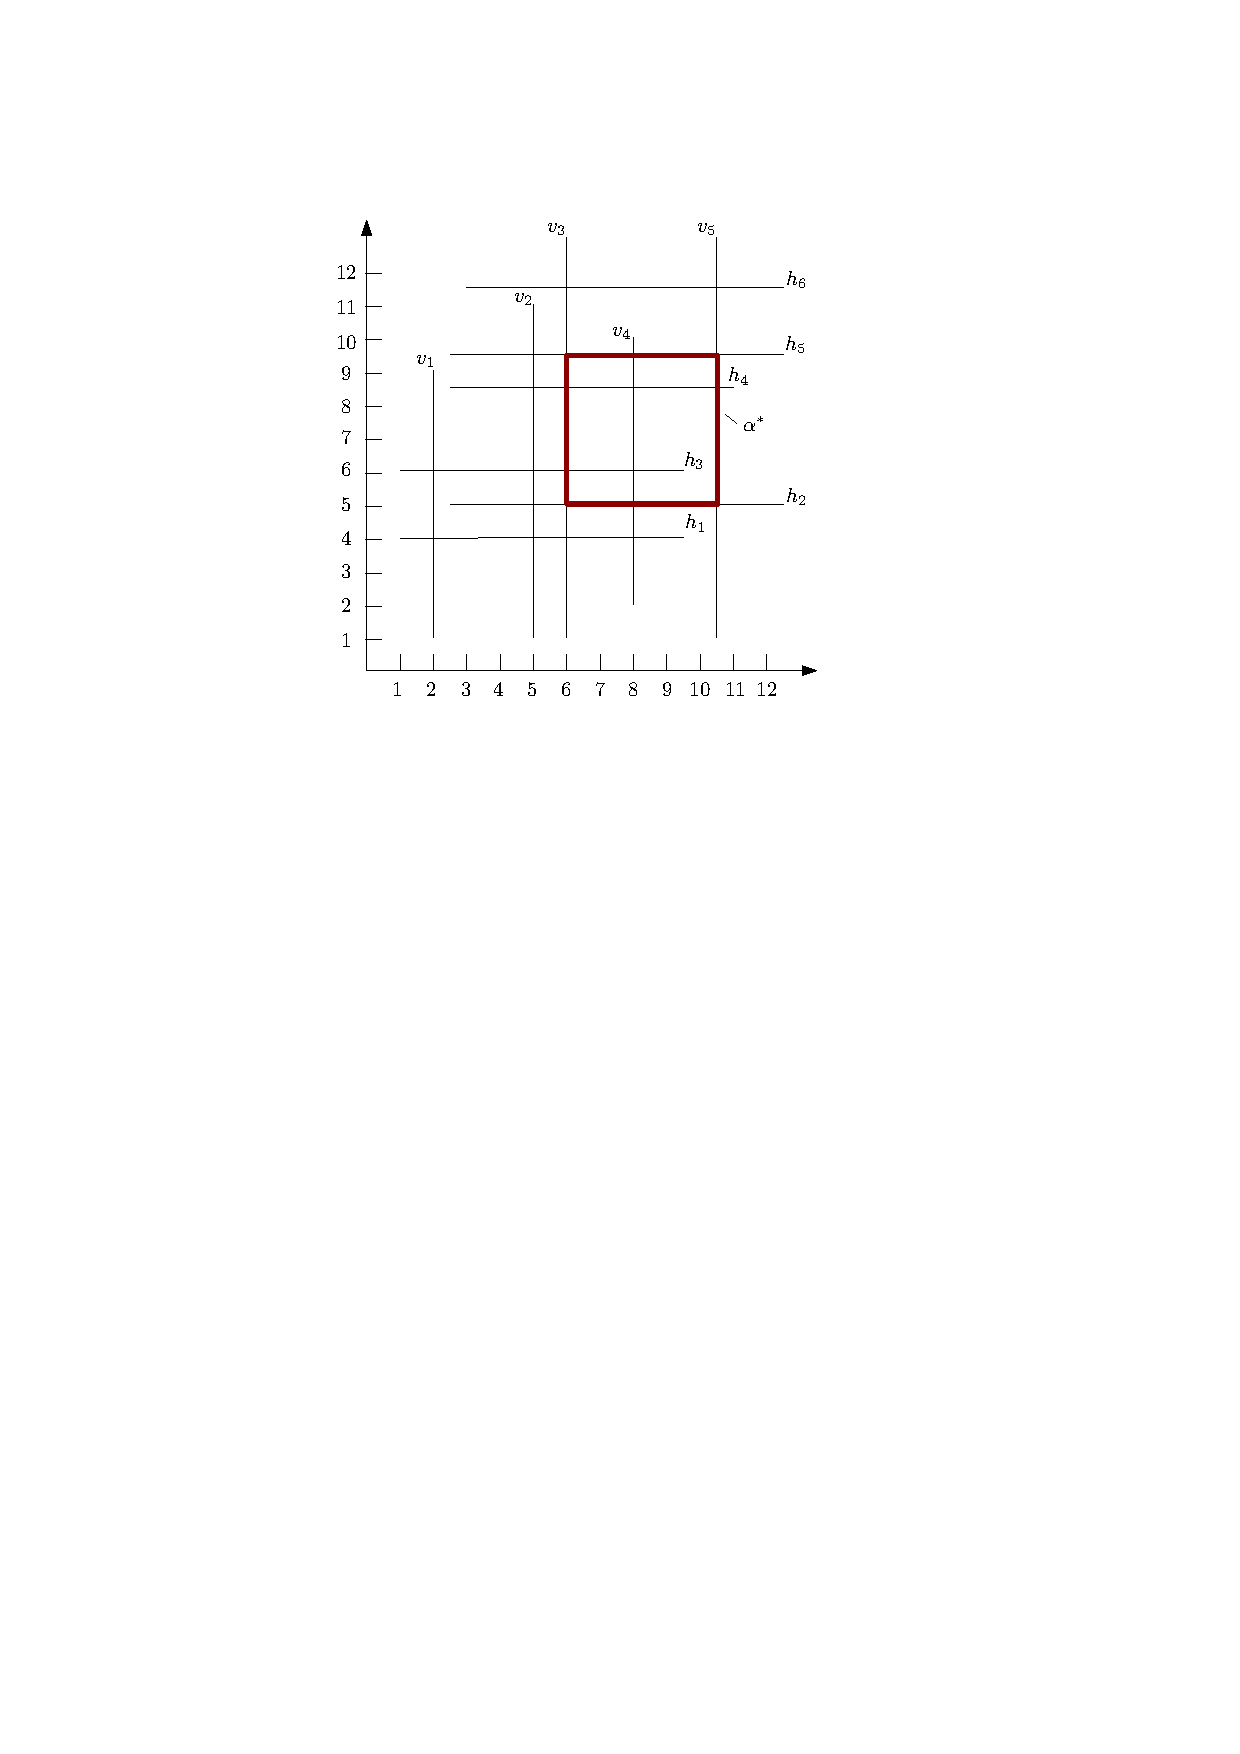
\includegraphics[height=45mm]{./artwork/alg-ex1-d} \\ 
        \hspace{-5mm} (a) $R_1$, $R_2$, $H$, and $V$ &
        \hspace{-4mm} (b) $R_1'$ and $R_2'$ &
        \hspace{-4mm} (c) $R_1'$, $R_2'$, $H$, and $V$ &
        \hspace{-4mm} (d) $R_1^*$, $R_2^*$ ($= \emptyset$), and $H$
    \end{tabular}
    \figcapup 
    \caption{Finding H-V $k$-SJ result tuples of type 1 ($k = 4$)} 
    \label{fig:hv:type1:ex}
    \figcapdown 
\end{figure*}

\section{H-V $k$-SJ: Result Tuples of Type 1} \label{sec:hv:type1}

As before, let $R_1, ..., R_{k-2}, H$, and $V$ be the input sets of the H-V $k$-SJ problem. Denote by $\J_1$ the set of type-1 result tuples defined in Section~\ref{sec:hv}. In this section, we aim to compute a set $\J^*$ satisfying
\myeqn{
    \J_1
    \subseteq
    \J^*
    \subseteq
    \J(R_1, ..., R_{k-2}, H, V) \label{eqn:hv:type1:J*}
}
where $\J(R_1, ..., R_{k-2}, H, V)$, let us recall, is the join result of the (whole) H-V $k$-SJ. Remember that the output size $\out$ is defined as $|\J(R_1, ..., R_{k-2}, H, V)|$. From $\J^*$, we will report only those $k$-tuples belonging to $\J_1$ and ignore the rest.

\extraspacing {\underline{\em Example 4.1.}} To illustrate our algorithm, we will utilize the running example in Figure~\ref{fig:hv:type1:ex}a, where $k = 4$, and $R_1 = \set{\alpha}$, $R_2 = \set{\beta_2, \beta_2}$, $H$ $=$ $\set{h_1,$ $h_2,$ $..., h_6}$, and $V = \set{v_1, v_2, ..., v_5}$. The set $\J_1$ contains the following tuples: $(\alpha, \beta_2, h_2, v_3)$, $(\alpha, \beta_2, h_2, v_5)$, $(\alpha, \beta_2, h_5, v_3)$, and $(\alpha,$ $\beta_2, h_5, v_6)$. \qed

\extraspacing {\bf Sets $\bm{R_1', R_2', ..., R'_{k-2}}$.} Fix any $i \in [k-2]$. For each rectangle $r \in R_i$, we compute four segments:
\myitems{
    \item $h_\bot$ (resp., $h_\top$): the lowest (resp., highest) segment in $H$ that crosses $r$;
    
    \item $v_\vdash$ (resp., $v_\dashv$): the leftmost (resp., rightmost) segment in $V$ that crosses $r$.
}
Define $r' = [x_\vdash, x_\dashv] \times [y_\bot, y_\top]$, where $x_\vdash$ (resp., $x_\dashv$) is the x-coordinate of $v_\vdash$ (resp., $v_\dashv$), and $y_\bot$ (resp., $y_\top$) is the y-coordinate of $h_\bot$ (resp., $h_\top$). We say that $r'$ is the {\em trimmed rectangle} of $r$, and conversely, $r$ is the {\em full rectangle} of $r'$. Note that $r'$ exists if and only if $r$ is crossed by at least one horizontal segment in $H$ and by at least one vertical segment in $V$. 

%Moreover, it is possible for $h_1$ and $h_2$ to be the same segment; same for $v_1$ and $v_2$. 

\vgap 

Construct
\myeqn{
    R_i' &=& \set{r' \mid r \in R_i \text{ and its trimmed rectangle $r'$ exists}}. \nn
}
Computing the ``segment $h_\bot$'' for each $r \in R_i$ is an instance of Problem $\mathscr{D}$ (the find-lowest version, with $H$ and $R_i$ as the input). By symmetry, so is the computation of $h_\top, v_\vdash$, and $v_\dashv$ segments for each $r \in R_i$. It thus follows from Section~\ref{sec:bricks} that $R_1', R_2', ..., R_{k-2}'$ can be produced in $O(kn \log n)$ total time.

\vgap

We now solve a $(k-2)$-SJ problem on the input $\set{R_1', R_2', ..., R_{k-2}'}$ using the algorithm $\A$ supplied (see Lemma~\ref{lmm:hv}). This $(k-2)$-SJ clearly has an input size at most $n$, and let us represent its result as $\J(R'_1, R'_2, ..., R'_{k-2})$. We prove in Appendix~\ref{app:hv}:

\begin{lemma} \label{lmm:hv:type1:recur-output}
    $|\J(R_1', R'_2, ..., R'_{k-2})| \le \out$.
\end{lemma}

As a corollary of Lemma~\ref{lmm:hv:type1:recur-output}, the $(k-2)$-SJ can be settled in $F_{k-2}(n, \out)$ time.

\extraspacing {\underline{\em Example 4.2.}} Figure~\ref{fig:hv:type1:ex}b shows the rectangles in $R'_1 = \set{\alpha'}$ and $R'_2$ $=$ $\{\beta'_1,$ $\beta'_2\}$. For instance, $\alpha'$, which is trimmed from rectangle $\alpha$, is decided by $h_\bot$ $=$ $h_2$, $h_\top$ $=$ $h_6$, $v_\vdash = v_3$, and $v_\dashv = v_5$. The $(k-2)$-SJ on $R'_1$ and $R'_2$ returns $\J(R_1', R'_2, ..., R'_{k-2}) = \set{(\alpha', \beta_1'), (\alpha', \beta_2')}$.
\qed

%\yf{example}

\extraspacing {\bf Generating $\bm{\J^*}$.} Take any $(k-2)$-tuple $\bm{t} = (r'_1, r'_2, ...,$ $r'_{k-2}) \in \J(R_1', R'_2, ..., R'_{k-2})$. The reader should recall from Section~\ref{sec:bricks} that
\myitems{
    \item $B_\bm{t}$ is $\bigcap_{i=1}^{k-2} \bm{t}[i] = \bigcap_{i=1}^{k-2} r'_i$;
    \item $\gleft(\bm{t})$ is the $r'_i$ ($1 \le i \le k-2$) with $\xleft(r'_i) = \xleft(B_\bm{t})$;
    \item $\gbot(\bm{t})$ is the $r'_i$ ($1 \le i \le k-2$) with $\ybot(r'_i) = \ybot(B_\bm{t})$.
}
We now introduce:
\myeqn{
    \dcross_H(\bm{t}) = \set{h \in H \mid \text{$h$ crosses both $B_\bm{t}$ and $\gbot(\bm{t})$}} \label{eqn:dcross-H} \\
    \dcross_V(\bm{t}) = \set{v \in V \mid \text{$v$ crosses both $B_\bm{t}$ and $\gleft(\bm{t})$}}. \nn
    %\label{eqn:dcross-H} 
}
The prefix ``d-'' stands for ``double''. These sets have important properties as stated in the next lemma, whose proof can be found in Appendix~\ref{app:hv}:

\begin{lemma} \label{lmm:hv:type1:properties}
    %Let $r_i$ be the full rectangle of $r_i'$ for each $i \in [k-2]$.
    All the following statements are true:
    \myenums{
        \item Consider any $(k-2)$-tuple $\bm{t} \in \J(R_1', R'_2, ..., R'_{k-2})$. Let $r_i$ ($i$ $\in$  $[k-2]$) be the full rectangle of $\bm{t}[i]$. Then, for any $h \in \dcross_H(\bm{t})$ and any $v \in \dcross_V(\bm{t})$, the $k$-tuple $(r_1, r_2,$ $...,$ $r_{k-2}, h, v)$ must belong to $\J(R_1, ..., R_{k-2}, H, V)$.
        
        \item Consider any a $k$-tuple $(r_1, r_2, ..., r_{k-2}, h, v) \in \J_1$. Let $r'_i$ ($i \in [k-2])$ be the trimmed rectangle of $r_i$, and set $\bm{t} = (r'_1, r'_2, ...,$ $r'_{k-2})$. Then, we must have 
        \myitems{
            \item $\bm{t} \in \J(R_1', R'_2, ..., R'_{k-2})$;
            \item $h \in \dcross_H(\bm{t})$ and $v \in \dcross_V(\bm{t})$. 
        }
        
        \vspace{2mm}
        
        \item $\sum_{\bm{t}} |\dcross_H(\bm{t})| \le \out$ and $\sum_{\bm{t}} |\dcross_V(\bm{t})| \le \out$, where the two summations are over all $\bm{t} \in \J(R_1', R'_2, ..., R'_{k-2})$.
    }
\end{lemma}

\noindent {\underline{\em Example 4.3.} Let us examine, in turn, the two 2-tuples $\bm{t}_1 = (\alpha', \beta_1')$ and $\bm{t}_2 = (\alpha', \beta_2')$ in $\J(R_1', R_2')$. For $\bm{t}_1$, $B_{\bm{t}_1}$ is the rectangle \ttt{ABCD} in Figure~\ref{fig:hv:type1:ex}c, and $\gleft(\bm{t}_1) = \gbot(\bm{t}_1) = \alpha'$. Accordingly, $\dcross_H(\bm{t}_1) = \set{h_2}$ and $\dcross_V(\bm{t}_1) = \set{v_3}$. For $\bm{t}_2$, $B_{\bm{t}_2}$ is the rectangle \ttt{AEFG}, and $\gleft(\bm{t}_2) = \gbot(\bm{t}_2) = \alpha'$. Accordingly, $\dcross_H(\bm{t}_2) = \set{h_2, h_4, h_5}$ and $\dcross_V(\bm{t}_2) = \set{v_3, v_5}$.
\qed

\vgap 

Equipped with Lemma~\ref{lmm:hv:type1:properties}, we generate our target $\J^*$ as follows:

\mytab{
    \> {\bf algorithm generate-$\J^*$} \\
    \> 1.\> $\J^* = \emptyset$ \\
    \> 2.\> {\bf for} each $(k-2)$-tuple $\bm{t} \in \J(R'_1, ..., R'_{k-2})$ {\bf do} \\
    \> 3.\>\> $r_i \leftarrow$ the full rectangle of $\bm{t}[i]$, for each $i \in [k-2]$ \\
    \> 4.\>\> {\bf for} each $(h, v) \in \dcross_H(\bm{t}) \times \dcross_V(\bm{t})$ {\bf do} \\
    \> 5.\>\>\> add $(r_1, ..., r_{k-2}, h, v)$ to $\J^*$
}


By statements (1) and (2) of Lemma~\ref{lmm:hv:type1:properties}, the set $\J^*$ thus computed indeed satisfies \eqref{eqn:hv:type1:J*}. Furthermore, if we are given $\dcross_H(\bm{t})$ and $\dcross_V(\bm{t})$ for each $\bm{t}$, the above algorithm runs in $O(1 + |\J(R'_1, ..., R'_{k-2})| + k \cdot |\J^*|) = O(1 + k \cdot \out)$ time, where the derivation used \eqref{eqn:hv:type1:J*} and Lemma~\ref{lmm:hv:type1:recur-output}.

\vgap 

The rest of the section will focus on how to prepare the sets $\dcross_H(\bm{t})$ of all $\bm{t} \in \J(R_1', ..., R_{k-2}')$ in $O(n \log n + k \cdot \out)$ time. An analogous method can be used to compute the sets $\dcross_V(\bm{t})$ of all $\bm{t}$ within the same time complexity.

\extraspacing {\underline{\em Example 4.4.} In our running example, the $\J^*$ computed includes 7 tuples: $(\alpha, \beta_1, h_2, v_3)$, and $\{\alpha\} \times \{\beta_2\} \times \set{h_2, h_4, h_5} \times \set{v_3, v_5}$. All these 7 tuples belong to $\J(R_1, R_2, H, V)$ and include the 4 tuples in $\J_1$ (see Example 4.1).
\qed

\extraspacing {\bf Sets $\bm{R^*_1, R^*_2, ..., R^*_{k-2}}$.} Fix any $i \in [k-2]$. Define for each $r' \in R_i'$:
\myeqn{
    \maxtop(r') &=& \max_{\bm{t} \in \J(R'_1, ..., R'_{k-2}): \gbot(\bm{t}) = r'} \ytop(B_\bm{t}). 
    \label{eqn:hv:type1:maxtop}
}
We set $\maxtop(r')$ to $-\infty$, if no $\bm{t} \in \J(R'_1, ..., R'_{k-2})$ has $r'$ as the $\gbot(\bm{t})$. When $\maxtop(r') \ne -\infty$, assuming $r' = [x_1, x_2] \times [y_1, y_2]$, we introduce a rectangle
\myeqn{
    r^* &=& [x_1, x_2] \times [y_1, \maxtop(r')]. \label{eqn:hv:type1:topsliced}
}
and call it the {\em top-sliced rectangle} of $r'$.

%\vgap

\extraspacing {\underline{\em Example 4.5.} Recall from Example 4.3 that rectangle $\alpha'$ is both $\gbot(\bm{t}_1)$ and $\gbot(\bm{t}_2)$. Thus, $\maxtop(\alpha') = \max\{\ytop(B_{\bm{t}_1}),$ $\ytop(B_{\bm{t}_2})\} = \max\{6, 9.5\} = 9.5$. The top-sliced rectangle of $\alpha'$ is the rectangle $\alpha^*$ in Figure~\ref{fig:hv:type1:ex}d. Rectangles $\beta'_1$ and $\beta'_2$ do not have top-sliced rectangles.
\qed

\vgap 

Next, we construct from $R_i'$ a new set of rectangles: 
\myeqn{
    R^*_i = \set{r^* \mid r' \in R_i' \text{ and its top-sliced rectangle $r^*$ exists}}. \label{eqn:hv:type1:R*}
}
In Appendix~\ref{app:hv}, we show how to compute produce $R^*_1, ..., R^*_{k-2}$ together in $O(n + k \cdot \out)$ total time.

\vgap 

Our focus lies specifically on the sets $\cross_H(r^*)$ of the rectangles $r^*$ in $R^*_i$, where $\cross_H(r^*)$ --- defined in \eqref{eqn:cross} --- is the set of segments in $H$ crossing $r^*$. The following lemma, proven in Appendix~\ref{app:hv}, presents some useful properties of these sets. 

\begin{lemma} \label{lmm:hv:type1:cross-r*}
    Both statements below are true: 
    \myenums{
        \item $\sum_{i=1}^{k-2} \sum_{r^* \in R^*_i} |\cross_H(r^*)| \le \out$.
        
        \item Consider any tuple $\bm{t} \in \J(R'_1, ..., R'_{k-2})$. Let $r' = \gbot(\bm{t})$ and $r^*$ be the top-sliced rectangle of $r'$. Then, we have $\dcross_H(\bm{t})$ $\subseteq \cross_H(r^*)$. Furthermore, if the (horizontal) segments of $\cross_H(r^*)$ are sorted in ascending order of their y-coordinates, then $\dcross_H(\bm{t})$ includes a prefix of the sorted order.
    }
\end{lemma}

\extraspacing {\underline{\em Example 4.6.}} It is clear from Figure~\ref{fig:hv:type1:ex}d that $\cross_H(\alpha^*)$ contains $h_2, h_4$, and $h_5$, sorted in ascending order of y-coordinate. Recall that 
$\gbot(\bm{t}_1) = \gbot(\bm{t}_2) = \alpha'$. Both $\dcross_H(\bm{t}_1) = \set{h_2}$ and $\dcross_H(\bm{t}_2) = \set{h_2, h_4, h_5}$ are prefixes of the sorted list, as is consistent with Lemma~\ref{lmm:hv:type1:cross-r*}.
\qed

Finding the $\cross_H(r^*)$ sets of all $r^* \in R^*_i$ is an instance of the find-all-sorted version of Problem $\mathscr{D}$ (with $H$ and $R^*_i$ as the input). Statement (1) of Lemma~\ref{lmm:hv:type1:cross-r*}, as well as the discussion in Section~\ref{sec:bricks}, assures us that the total time to do so for all $R^*_1, ..., R^*_{k-2}$ is bounded by $O(k n \log n + \out)$. Note that, for each $\cross_H(r^*)$ computed, the (horizontal) segments therein have been sorted in ascending order of y-coordinate.


\extraspacing {\bf Computing the ``d-cross'' Sets.} We are ready to compute $\dcross_H(\bm{t})$, defined in \eqref{eqn:dcross-H}, for any $\bm{t} \in \J(R'_1, ..., R'_{k-2})$, thanks to Statement (2) of Lemma~\ref{lmm:hv:type1:cross-r*}. First, compute $B_\bm{t}$, obtain the rectangle $r' = \gbot(\bm{t})$, and fetch the (already computed) top-sliced rectangle $r^*$ of $r'$; these steps require $O(k)$ time. Then, scan the segments in $\cross_H(r^*)$ in ascending order of their y-coordinates. For each segment $h$ scanned, check whether $h$ belongs to $\dcross_H(\bm{t})$, namely, whether $h$ crosses $B_\bm{t}$ (the reader can verify that $h$ must cross $\gbot(\bm{t})$); this can be done in constant time. Abort the scan as soon as $h \notin \dcross_H(\bm{t})$. This way, we produce $\dcross_H(\bm{t})$ in $O(k + |\dcross_H(\bm{t})|)$ time. Doing so for all $\bm{t} \in \J(R'_1, ..., R'_{k-2})$ takes $O(k \cdot |\J| + \sum_\bm{t} |\dcross_H(t)|) = O(k \cdot \out)$ time, where the derivation used Lemma~\ref{lmm:hv:type1:recur-output} and statement (3) of Lemma~\ref{lmm:hv:type1:properties}.

\vgap 

We conclude that $\J_1$ --- the set of type-1 result tuples --- can be computed in $F_{k-2}(n, \out) + O(kn \log n +  k \cdot \out)$ time.


\begin{figure*}
    \begin{tabular}{cccc}
        \hspace{-5mm}
        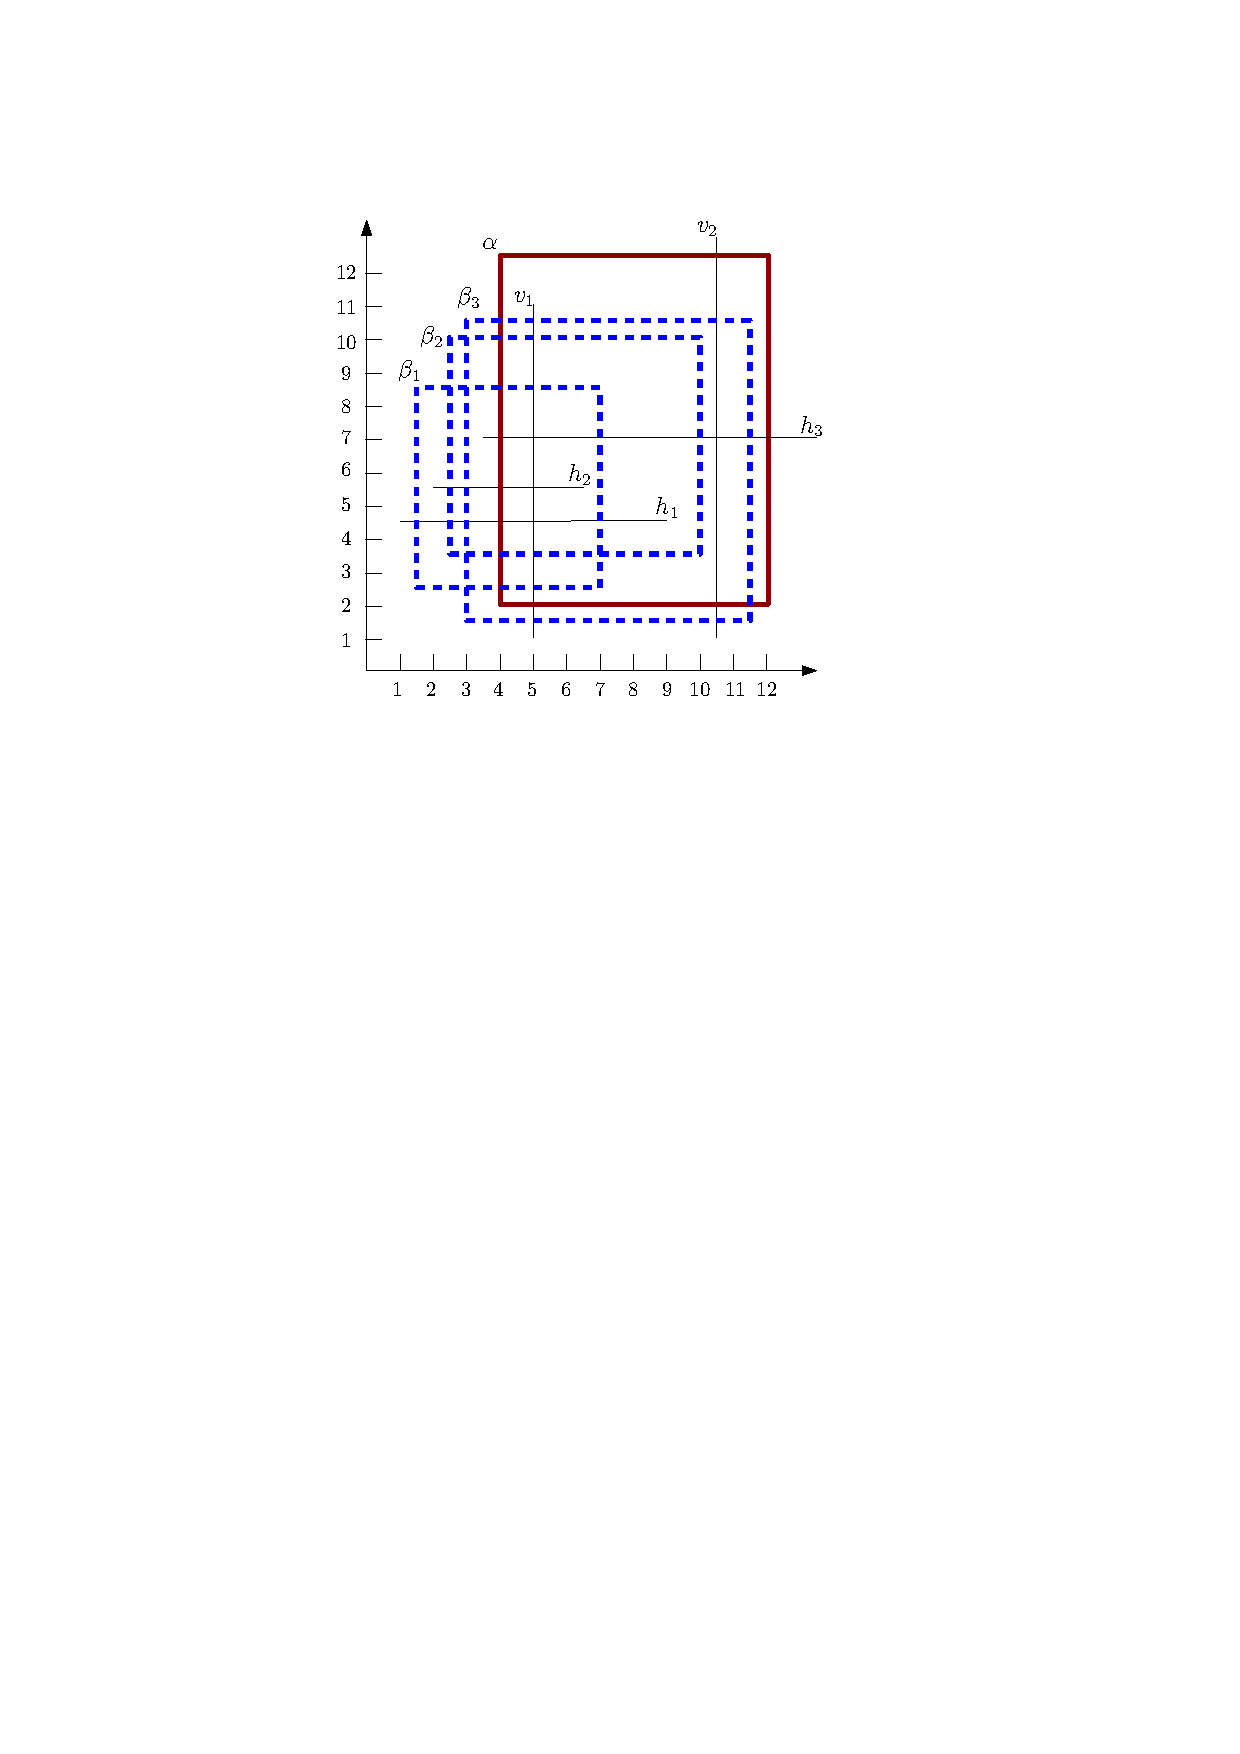
\includegraphics[height=45mm]{./artwork/alg-ex2-a} &
        \hspace{-4mm}
        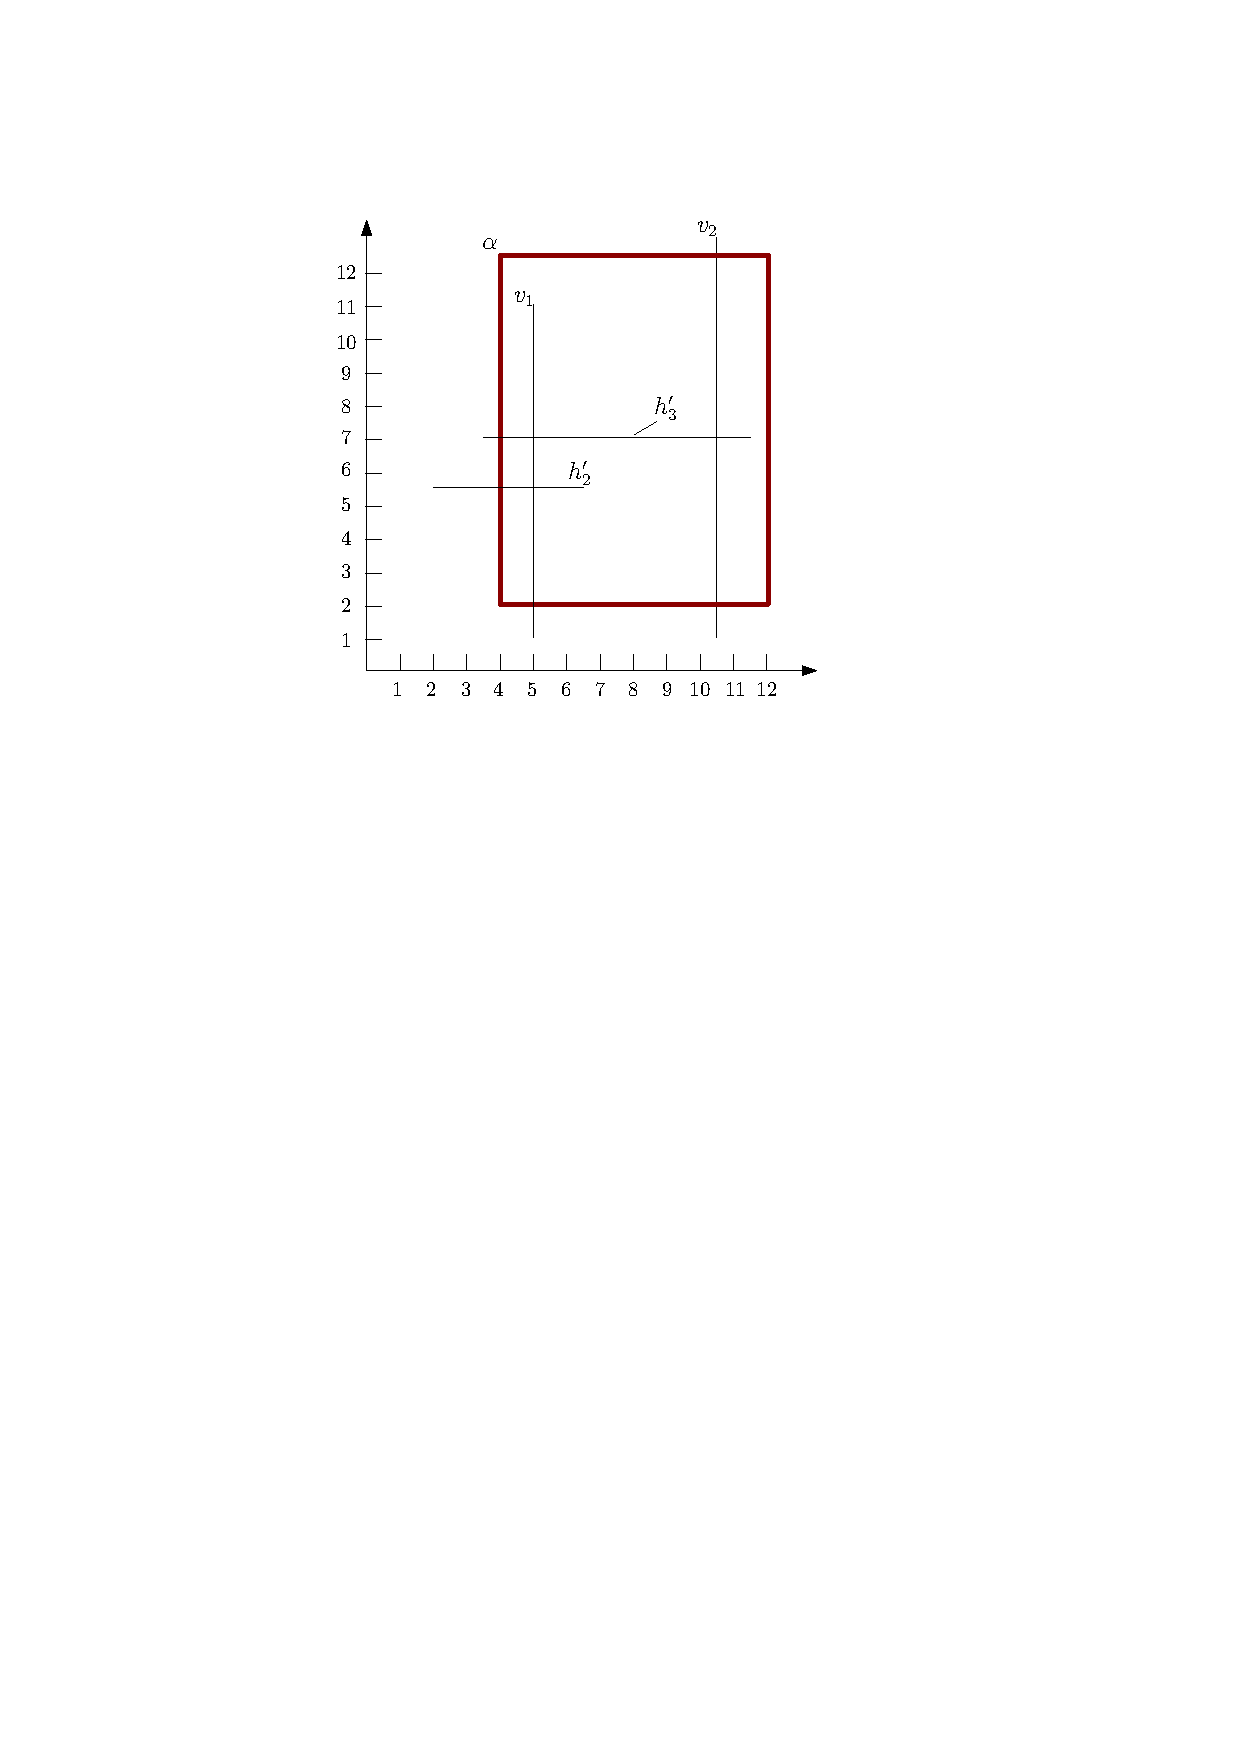
\includegraphics[height=45mm]{./artwork/alg-ex2-b} &
        \hspace{-4mm}
        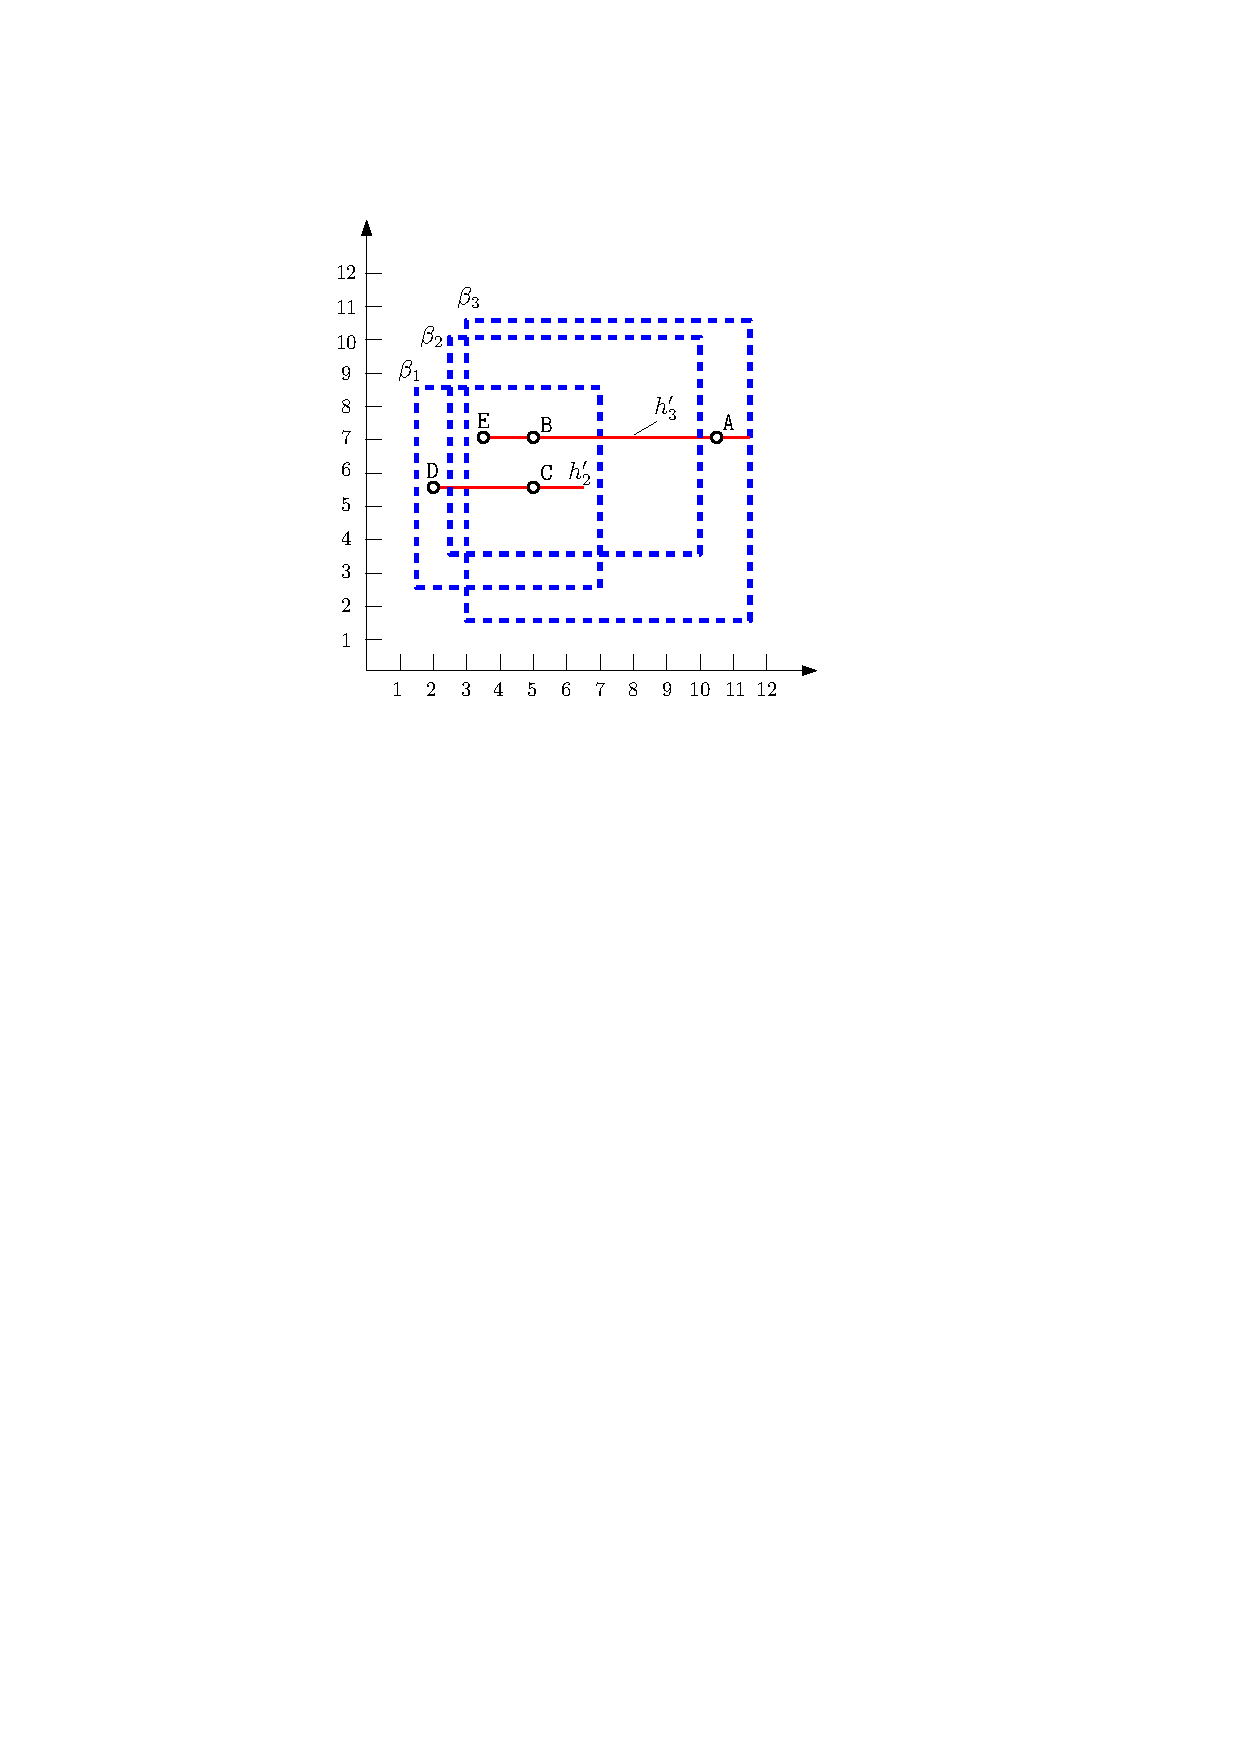
\includegraphics[height=45mm]{./artwork/alg-ex2-c} &
        \hspace{-4mm}
        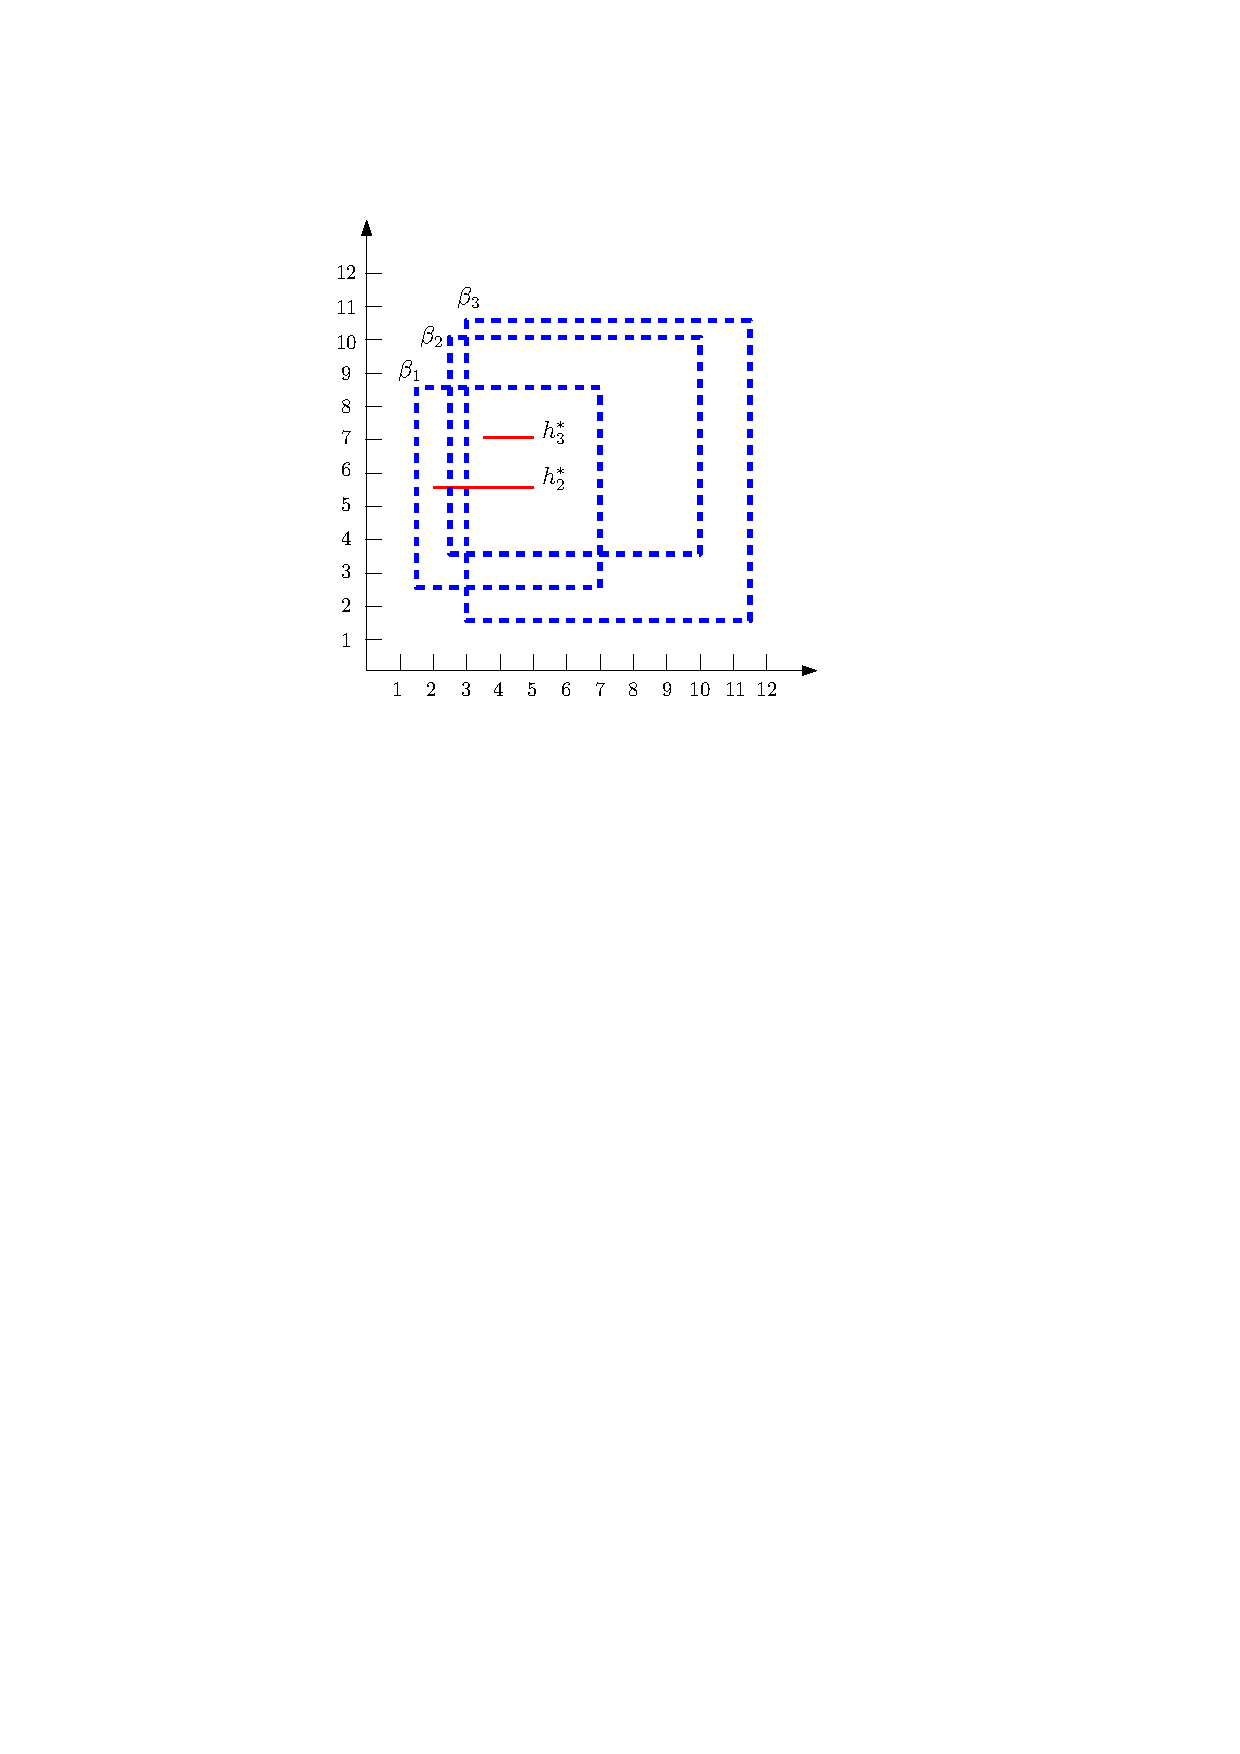
\includegraphics[height=45mm]{./artwork/alg-ex2-d} \\
        \hspace{-5mm} (a) $R_1$, $R_2$, $H$, and $V$ &
        \hspace{-4mm} (b) $R_1$, $H'$, and $V$ &
        \hspace{-4mm} (c) $R_2$, $H'$, and $V$ &
        \hspace{-4mm} (d) $R_2$ and $H^*$
    \end{tabular}
    \figcapup
    \caption{Finding H-V $k$-SJ result tuples of type 2 ($k = 4$)}
    \label{fig:hv:type2:ex}
    \figcapdown
\end{figure*}


\section{H-V $k$-SJ: Result Tuples of Type 2} \label{sec:hv:type2}

Still, denote by $R_1, ..., R_{k-2}, H$, and $V$ the input sets of the H-V $k$-SJ problem. This section will explain how to find the result tuples of Type 2 as defined in Section~\ref{sec:hv}.

\vgap

As mentioned before, for a result tuple $(r_1, ..., r_{k-2}, h, v)$ of this type, a rectangle $r_i$, for some $i \in [k-2]$, covers an endpoint of $h$ or $v$ or both. As (i) there are $k-2$ choices for $i$ and (ii) $h$ and $v$ together have four endpoints, we can divide Type 2 further into $4(k-2)$ ``sub-types'': in subtype 1 (resp., 2), $r_1$ covers the left (resp., right) endpoint of $h$, in subtype 3 (resp., 4), $r_1$ covers the bottom (resp., top) endpoint of $v$, in subtype 5 (resp., 6), $r_2$ covers the left (resp., right) endpoint of $h$, etc. It is possible for the result tuple to belong to multiple sub-types simultaneously. Next, we will focus on producing the result tuples of a particular sub-type:
\myeqn{
    \J_2  &=& \{(r_1, ..., r_{k-2}, h, v) \in \J(R1, ..., R_{k-2}, H, V) \mid \text{$r_{k-2}$ covers} \nn \\[-0.5mm]
    && \text{the left endpoint of $h$}\}. \label{eqn:hv:type2:J2}
}
The other sub-types can be found analogously.

\vgap

A remark is in order about duplicate removal. By finding each sub-type separately, we may see the same result tuple multiple times (precisely, up to $4(k-2)$ times) in the whole algorithm. However, this does not mean that the tuple needs to be reported multiple times. Whenever a type-2 result tuple is found, we can immediately decide in $O(k)$ time all the sub-types it belongs to. To avoid outputting the tuple more than once, we can enforce a policy to designate a specific sub-type for outputting. One such policy is the following: among all sub-types that the tuple belongs to, identify the one with the smallest sub-type number $t$ (an integer from 1 to $4(k-2)$); report the tuple only when we are computing the particular sub-type $t$.

\extraspacing {\underline{\em Example 5.1.}} To illustrate our algorithm, we will utilize the running example in Figure~\ref{fig:hv:type2:ex}a, where $k = 4$, and $R_1 = \set{\alpha}$, $R_2 = \set{\beta_2, \beta_2, \beta_3}$, $H$ $=$ $\set{h_1,$ $h_2,$ $h_3}$, and $V = \set{v_1, v_2}$. The set $\J_2$ contains the following tuples: $(\alpha, \beta_1, h_2, v_1)$, $(\alpha, \beta_1, h_3, v_1)$, $(\alpha, \beta_2, h_3, v_1)$, $(\alpha, \beta_3, h_3, v_1)$, and $(\alpha, \beta_3, h_3, v_2)$. \qed


\extraspacing {\bf Set $\bm{H'}$.} Take any horizontal segment $h = [x_1, x_2] \times y \in H$. Recall from Section~\ref{sec:bricks} that a left-end covering rectangle of $h$ is a rectangle covering the left endpoint of $h$. 
Let $p$ be the rightmost point on $h$ such that at least one left-end covering rectangle of $h$ in $R_{k-2}$ covers $p$. This $p$ exists if and only if $h$ has at least one left-end covering rectangle in $R_{k-2}$. If $p$ exists and has coordinates $(x, y)$, we refer to the segment $h' = [x_1, x] \times y$ as the {\em trimmed segment} of $h$; conversely, we call $h$ the {\em full segment} of $h'$.

\vgap 

Construct
\myeqn{
    H' &=& \{h' \mid h \in H \text{ and its trimmed segment $h'$ exists} \}. \nn
}
The construction is an instance of Problem $\mathscr{C}$ (with $H$ and $R_{k-2}$ as the input) and finishes in $O(n \log n)$ time based on the discussion in Section~\ref{sec:bricks}.

\vgap 

Now, solve a $(k-1)$-SJ problem on the input $\set{R_1, ..., R_{k-3}, H', V}$ using the algorithm $\A$ supplied (by Lemma~\ref{lmm:hv}). Let $\J(R_1, ...,$ $R_{k-3}, H', V)$ represent the result of this $(k-1)$-SJ, whose input size is at most $n$. Given the lemma below (which is proved in Appendix~\ref{app:hv}), we assert that $\J(R_1, ..., R_{k-3}, H', V)$ can be computed in $F_{k-1}(n, \out)$ time.

\begin{lemma} \label{lmm:hv:type2:recur-output}
    $|\J(R_1, ..., R_{k-3}, H', V)| \le \out$.
\end{lemma}

\noindent {\underline{\em Example 5.2.}} Segment $h_1$ has no left-covering rectangle in $R_2$ (see Figure~\ref{fig:hv:type2:ex}a) and thus has no trimmed segment. Segment $h_2$ has one left-covering rectangle in $R_2$, which is $\beta_1$. As the entire $h_2$ is covered by $\beta_1$, it is equivalent to its trimmed segment $h_2'$; see Figure~\ref{fig:hv:type2:ex}b. Segment $h_3$ has two left-covering rectangles in $R_2$, which are $\beta_2$ and $\beta_3$. The right endpoint of its trimmed segment $h_3'$, as shown in Figure~\ref{fig:hv:type2:ex}b, is decided by the right edge of $\beta_3$. Therefore, $H' = \set{h_2', h_3'}$. It is clear from Figure~\ref{fig:hv:type2:ex}b that $\J(R_1, H', V)$ has 3 tuples: $\bm{t}_1 = (\alpha, h_2', v_1), \bm{t}_2 = (\alpha, h_3', v_1)$, and $\bm{t}_3 = (\alpha, h_3', v_2)$.
\qed

\extraspacing {\bf Generating $\bm{\J_2}$.} Take any $(k-1)$-tuple $\bm{t} = (r_1, ..., r_{k-3}, h', v) \in \J(R_1, ..., R_{k-3}, H', V)$. Note that $B_\bm{t}$ --- defined in \eqref{eqn:B_t} --- is a point (due to $h'$ and $v$). Suppose $h' = [x_1, x_2] \times y$ and $B_\bm{t} = (x, y)$, we define the {\em effective horizontal segment} of $\bm{t}$ as the horizontal segment $[x_1, x] \times y$. This allows us to define
\myeqn{
    \contained_{R_{k-2}}(\bm{t}) &=& \{r \in R_{k-2} \mid \text{ the effective horizontal } \nn \\[-1mm]
    && \text{segment of $\bm{t}$ is contained in $r$}   \}
    \label{eqn:type2:contained-t}
}
The above should not be confused with \eqref{eqn:contained}, where the ``$\contained$'' function takes a segment as the parameter, rather than a tuple.

\extraspacing {\underline{\em Example 5.3.}} Consider the tuples $\bm{t}_1$, $\bm{t}_2$, and $\bm{t}_3$ of $ \J(R_1, H', V)$ given in Example 5.2. For $\bm{t}_1 = (\alpha, h_2', v_1)$, its effective horizontal segment is $\texttt{DC}$ (see Figure~\ref{fig:hv:type2:ex}b). For $\bm{t}_2 = (\alpha, h_3', v_1)$, its effective horizontal segment is \texttt{EB}. For $\bm{t}_3 = (\alpha, h_3', v_2) \in \J(R_1, H', V)$, its effective horizontal segment is \texttt{EA}. Accordingly, as can be seen from Figure~\ref{fig:hv:type2:ex}c,
$\contained_{R_{k-2}}(\bm{t}_1) = \contained_{R_2}(\bm{t}_1) = \set{\beta_1}$, $\contained_{R_2}(\bm{t}_2) = \set{\beta_1, \beta_2, \beta_3}$, and $\contained_{R_2}(\bm{t}_3) = \set{\beta_3}$.
\qed

\vgap 

We prove the next lemma in Appendix~\ref{app:hv} (to avoid confusion, the reader may want to be reminded that, for each $\bm{t} \in \J(R_1, ..., R_{k-3}, H', V)$, $\bm{t}[k-2]$ is a horizontal segment and $\bm{t}[k-1]$ is a vertical segment).

\begin{lemma} \label{lmm:hv:type2:properties}
    All the following statements are true:
    \myenums{
        \item Consider any $(k-1)$-tuple $\bm{t} \in \J(R_1, ..., R_{k-3}, H', V)$. Denote by $h$ the full segment of $\bm{t}[k-2]$. Then, for any $r \in \contained_{R_{k-2}}(\bm{t})$, the $k$-tuple $(\bm{t}[1], ..., \bm{t}[k-3], r, h, \bm{t}[k-1])$ must belong to $\J_2$.
        
        \item Consider any $k$-tuple $(r_1, ..., r_{k-2}, h, v) \in \J_2$. Let $h'$ be the trimmed segment of $h$ and set $\bm{t} = (r_1, ..., r_{k-3}, h', v)$. Then, $\bm{t} \in \J(R_1, ..., R_{k-3}, H', V)$ and $h' \in \contained_{R_{k-2}}(\bm{t})$.
        
        \item $\sum_{\bm{t}} |\contained_{R_{k-2}}(\bm{t})| \le \out$, where the summation is over all $\bm{t} \in \J(R_1, ..., R_{k-3}, H', V)$.
    }
\end{lemma}


Equipped with Lemma~\ref{lmm:hv:type1:properties}, we generate our target $\J_2$ as follows:

\mytab{
    \> {\bf algorithm generate-$\J_2$} \\
    \> 1.\> $\J_2 = \emptyset$ \\
    \> 2.\> {\bf for} each $(k-2)$-tuple $\bm{t} \in \J(R_1, ..., R_{k-3}, H', V)$ {\bf do} \\
    \> 3.\>\> $h \leftarrow$ the full segment of $\bm{t}[k-2]$ \\
    \> 4.\>\> {\bf for} each $r \in \contained_{R_{k-2}}(\bm{t})$ {\bf do} \\
    \> 5.\>\>\> add $(\bm{t}[1], ..., \bm{t}[k-3], r, h, \bm{t}[k-1])$ to $\J_2$
}

The correctness of the algorithm follows from statements (1) and (2) of Lemma~\ref{lmm:hv:type2:properties}. Furthermore, if we are given $\contained_{R_{k-2}}(\bm{t})$ for each $\bm{t}$, statement (3) of Lemma~\ref{lmm:hv:type2:properties}
assures us that the algorithm runs in $O(1 + |\J(R_1, ..., R_{k-3}, H', V)| + k \sum_\bm{t} |\contained_{R_{k-2}}(\bm{t})|) = O(1 + k \cdot \out)$ time, where the derivation used Lemma~\ref{lmm:hv:type2:recur-output} and statement (3) of Lemma~\ref{lmm:hv:type2:properties}.

\extraspacing {\underline{\em Example 5.4.}} For $\bm{t}_1 = (\alpha, h_2', v_1)$, first find the full segment of $h_2'$, which is $h_2$. As $\beta_1$ is the only rectangle in $\contained_{R_2}(\bm{t}_1)$, Line 5 of the algorithm adds tuple $(\alpha, \beta_1, h_2, v_1)$ to $\J_2$. For $\bm{t}_2 = (\alpha, h_3', v_1)$, the full segment of $h_3'$ is $h_3$. As $\contained_{R_2}(\bm{t}_2) = \set{\beta_1, \beta_2, \beta_3}$, Line 5 adds $(\alpha, \beta_1, h_3, v_1)$, $(\alpha, \beta_2, h_3, v_1)$, and $(\alpha, \beta_3, h_3, v_1)$ to $\J_2$. Finally, the processing of $\bm{t}_3 = (\alpha, h_3', v_2)$ adds $(\alpha, \beta_3, h_3, v_2)$ to $\J_2$.
\qed

\extraspacing {\bf Set $\bm{H^*}$.} 
For each segment $h' \in H'$, define
\myeqn{
    \minleft(h') = \min_{\substack{\text{$\bm{t} \in \J(R_1, ..., R_{k-3}, H', V):$}\\ \text{$\bm{t}[k-2] = h'$}}} \text{$x$-coordinate of $\bm{t}[k-1]$}. 
    \label{eqn:minleft}
}
We set $\minleft(h')$ to $\infty$, if no $\bm{t} \in \J(R_1, ..., R_{k-3}, H', V)$ has $h'$ in its field $\bm{t}[k-2]$. When $\minleft(h') \ne \infty$, assuming $h' = [x_1, x_2] \times y$, we introduce a horizontal segment
\myeqn{
    h^* &=& [x_1, \minleft(h')] \times y. \nn
}
and call it the {\em minimal segment} of $h'$.

\extraspacing {\underline{\em Example 5.5.}} As mentioned, $\J(R_1, H', V)$ has 3 tuples $\bm{t}_1$, $\bm{t}_2$, and $\bm{t}_3$. Both $\bm{t}_2 = (\alpha, h_3', v_1)$ and $\bm{t}_3 = (\alpha, h_3', v_2)$ have $h_3'$ as the horizontal segment. Therefore, $\minleft(h_3')$ equals the smaller between the x-coordinate of $v_1$ and that of $v_2$. The minimal segment $h_3^*$ of $h_3'$ is shown in Figure~\ref{fig:hv:type2:ex}(c). On the other hand, it is easy to verify that $\minleft(h_2')$ is the x-coordinate of $v_1$. The minimal segment $h_2^*$ of $h_2'$ is also shown in Figure~\ref{fig:hv:type2:ex}(c).
\qed

\vgap 

Next, we construct a new set of horizontal segments: 
\myeqn{
    H^* = \set{h^* \mid h' \in H' \text{ and its minimal segment $h^*$ exists}}. \label{eqn:hv:type2:H*}
}
This can be done in $O(n + k \cdot \out)$ time, as shown in Appendix~\ref{app:hv}. 

%Computing $H^*$ from $H'$ and $V$ is an instance of Problem $\mathscr{B}$, and can be achieved in $O(n \log n)$ as per the discussion from Section~\ref{sec:bricks}. 

\vgap 

We will utilize the sets $\contained_{R_{k-2}}(h^*)$ of the segments $h^*$ in $H^*$, where $\contained_{R_{k-2}}(h^*)$ --- defined in \eqref{eqn:contained} --- is the set of rectangles in $R_{k-2}$ containing $h^*$. These sets have some useful properties:

\begin{lemma} \label{lmm:hv:type2:contained-h*}
    Both statements below are true: 
    \myenums{
        \item $\sum_{h^* \in H^*} |\contained_{R_{k-2}}(h^*)| \le \out$.
        
        \item Consider any tuple $\bm{t} \in \J(R_1, ..., R_{k-3}, H', V)$. Set $h' = \bm{t}[k-2]$ and let $h^*$ be the minimal segment of $h'$. Then, $$\contained_{R_{k-2}}(\bm{t}) \subseteq \contained_{R_{k-2}}(h^*).$$ Furthermore, if the rectangles $r$ in $\contained_{R_{k-2}}(h^*)$ are sorted in descending order of $\xright(r)$, then $\contained_{R_{k-2}}(\bm{t})$ includes a prefix of the sorted order.
    }
\end{lemma}

The proof can be found in Appendix~\ref{app:hv}. 

\extraspacing {\underline{\em Example 5.6.}} It is clear from Figure~\ref{fig:hv:type2:ex}(d) that $\contained_{R_2}(h_3^*)$ has rectangles $\beta_3, \beta_2$, $\beta_1$, sorted in descending order of their right boundaries' x-coordinates. Consider $\bm{t}_2 = (\alpha, h_3', v_1)$ and $\bm{t}_3 = (\alpha, h_3', v_2)$. Segment $h_3^*$ is the minimal segment of $h_3'$. As stated in Lemma~\ref{lmm:hv:type2:contained-h*}, both $\contained_{R_2}(\bm{t}_2) = \set{\beta_1, \beta_2, \beta_3}$ and $\contained_{R_2}(\bm{t}_3) = \set{\beta_1}$ are prefixes of the sorted order of $\contained_{R_2}(h_3^*)$. Regarding $h_2^*$, it is the minimal segment of $h_2'$, and $\contained_{R_2}(h_2^*)$ contains only  $\beta_1$. For $\bm{t}_1 = (\alpha, h_2', v_1)$, $\contained_{R_2}(\bm{t}_1) = \set{\beta_1}$ is a (trivial) prefix of $\contained_{R_2}(h_2^*)$, as is consistent with the lemma.
\qed

Finding the $\contained_{R_{k-2}}(h^*)$ sets of all $h^* \in H^*$ is an instance of the find-all-sorted version of Problem $\mathscr{E}$ (with $H^*$ and $R_{k-2}$ as the input). The cost is $O(n \log n + \out)$ according statement (1) of Lemma~\ref{lmm:hv:type1:cross-r*} and the discussion in Section~\ref{sec:bricks}. Note that, for each $\contained_{R_{k-2}}(h^*)$ computed, the rectangles $r$ therein have been sorted in descending order of $\xright(r)$.


\extraspacing {\bf Computing the ``$\bm{\contained_{R_{k-2}}(t)}$'' Sets.} Statement (2) of Lemma~\ref{lmm:hv:type2:contained-h*} allows us to produce $\contained_{R_{k-2}}(\bm{t})$ --- defined in \eqref{eqn:type2:contained-t} --- for each $\bm{t} \in \J(R_1, ..., R_{k-3}, H', V)$ as follows. First, fetch the (already computed) minimal segment $h^*$ of $\bm{t}[k-2]$ in $O(1)$ time. Then, scan the rectangles $r$ of $\contained_{R_{k-2}}(h^*)$ in descending order of $\xright(r)$. For each $r$ scanned, check whether $r \in \contained_{R_{k-2}}(\bm{t})$, or equivalently, whether $r$ covers $B_\bm{t}$ (recall that $B_\bm{t}$ is a point); the cost of this inspection is $O(1)$. Abort the scan as soon as $r \notin
\contained_{R_{k-2}}(\bm{t})$. This way, $\contained_{R_{k-2}}(t)$ can be decided in $O(k + |\contained_{R_{k-2}}(\bm{t})|)$ time. Doing so for all $\bm{t} \in \J(R_1, ..., R_{k-3},$ $H', V)$ takes $O(k \cdot |\J| + \sum_\bm{t} |\contained_{R_{k-2}}(\bm{t})|) = O(k \cdot \out)$ time, where the derivation used Lemma~\ref{lmm:hv:type2:recur-output} and statement (3) of Lemma~\ref{lmm:hv:type2:properties}.



\vgap 

We conclude that $\J_2$ --- see \eqref{eqn:hv:type2:J2} --- can be computed in $F_{k-1}(n, \out) + O(n \log n +  k \cdot \out)$ time. Remember that, to generate the entire type-2 result, we need to repeat the algorithm $4(k-2)$ times (one for each sub-type). The total running time is therefore $O(k) \cdot (F_{k-1}(n, \out) + n \log n +  k \cdot \out)$, as claimed in Lemma~\ref{lmm:hv}.


\section{Settling $k$-SJ} \label{sec:ksj}

This section will tackle the $k$-SJ problem in its general form, where the input comprises $k \ge 3$ sets of rectangles $R_1, R_2, ..., R_k$. The join result $\J(R_1, R_2, ..., R_k)$ is the set of $k$-tuples $\bm{t} = (r_1, r_2, ..., r_k) \in R_1 \times R_2 \times ... \times R_k$ satisfying the condition that $B_\bm{t}$ --- which is $\bigcap_{i=1}^k r_i \ne \emptyset$ (see \eqref{eqn:B_t}) --- is non-empty.

\vgap 

Consider any result tuple $\bm{t} = (r_1, r_2, ..., r_k) \in \J(R_1, R_2, ..., R_k)$, and let $p$ be the top-left corner of $B_\bm{t}$. Depending on how $p$ is determined, we classify $\bm{t}$ into one of the two categories below: 
\myitems{
    \item {{\bf Cat.\ 1:}} $p$ is the top-left corner of $r_i$ for some $i \in [k]$. 
    
    \item {{\bf Cat.\ 2:}} $p$ is not a corner of any of $r_1, ..., r_k$. This means $p$ must be the intersection point between the top edge of some rectangle $r_i$ and the left edge of another rectangle $r_j$, where $i, j \in [k]$ and $i \ne j$.
}
Figure~\ref{fig:ksj:cats} illustrates a tuple of each category, assuming $k=4$. 

\vgap

The rest of this section serves as a proof of Theorem~\ref{thm:main-recur}. Theorem~\ref{thm:main-alg} is a corollary of Theorem~\ref{thm:main-recur}, as proved in Appendix~\ref{app:main-alg}. As stated in Theorem~\ref{thm:main-recur}, we are given an algorithm $\A$ that can solve any $(k-1)$-SJ problem in $F_{k-1}(n, \out)$ time, where $n$ and $\out$ are the input and output sizes, respectively. Equipped with $\A$, we will show how to find the result tuples of each category within the time complexity of \eqref{eqn:main:reccurrence}.

\extraspacing {\bf Category 1.} Given an $i \in [k]$, we denote by $\J^\cat_i$ the set of $k$-tuples $\bm{t} = (r_1, ..., r_k) \in \J(R_1, ..., R_k)$ such that the top-left corner of $B_\bm{t}$ is the top-left corner of $\bm{t}[i] = r_i$. We will show how to compute $\J^\cat_i$ for $i = k$; the set $\J^\cat_i$ of every other $i$ can be produced in the same manner.

\vgap 

For every $\bm{t} = (r_1, r_2, ..., r_k) \in \J^\cat_k$, the top-left corner of $r_k$ must be covered by all of $r_1, ..., r_{k-1}$. This observation motivates us to find $\J^\cat_i$ as follows. First, collect the set $P$ of top-left corners of all the rectangles in $R_k$. Remove from $P$ every point $p$ with the property that, there exists at least one $j \in [k-1]$ such that $p$ is covered by no rectangle in $R_j$. This requires solving $k-1$ instances of the detection version of Problem $\mathscr{A}$ (in each instance, the input includes $P$ together with a different $R_j$, $j \in [k-1]$); the cost is $O(k n \log n)$ by the discussion in Section~\ref{sec:bricks}.

\vgap 

Let $P'$ be the set of remaining points in $P$ after the aforementioned removal. Next, for each $j \in [k-1]$, solve the reporting version of Problem $\mathscr{A}$ by feeding $P'$ and $R_j$ as the input. This produces the set $\contained_{R_j}(p)$ for each point $p \in P'$, where $\contained_{R_j}(p)$ is defined in \eqref{eqn:contained} (treating $p$ as a degenerated ``horizontal segment'') and includes all rectangles of $R_j$ covering $p$. By the discussion in Section~\ref{sec:bricks}, the total cost of this step is bounded by
\myeqn{
    O\Big(kn \log n + \sum_{p \in P'} \sum_{j \in [k-1]} |\contained_{R_j}(p)| \Big). \label{eqn:ksj:cat1:help1}
}

We are ready to generate $\J^\cat_k$. Take any point $p \in P'$, and let $r \in R_k$ be the rectangle with $p$ as the top-left corner. For every $(k-1)$-tuple
\myeqn{
    (r_1, ..., r_{k-1}) \in \contained_{R_1}(p) \times ... \times \contained_{R_{k-1}}(p) \nn
    %\label{eqn:ksj:cat1:help2}
}
we add $(r_1, ..., r_{k-1}, r)$ to $\J^\cat_k$. Performing the above for all $p \in P'$ generates the whole $\J^\cat_k$ in $O(1 + |\J^\cat_k|)$ time. The way $P'$ is computed ensures that $\contained_{R_j}(p) \ne \emptyset$ for each $j \in [k-1]$. Hence, $\sum_{j \in [k-1]} |\contained_{R_j}(p)| \le \prod_{j \in [k-1]} |\contained_{R_j}(p)|$, which implies that \eqref{eqn:ksj:cat1:help1} is bounded by $O(kn \log n + k \cdot |\J^\cat_k|) = O(kn \log n + k \cdot \out)$ .

\vgap 

Therefore, the total time of computing all of $\J^\cat_1, ..., \J^\cat_k$ is $O(k) \cdot (kn \log n + k \cdot \out)$. A category-1 result tuple $\bm{t}$ may be seen more than once (this happens if the top-left corner of $B_\bm{t}$ is the top-left corner of more than one rectangle in $\bm{t}$). Duplicate removal can be implemented at no extra cost asymptotically, following the ideas explained in Section~\ref{sec:hv:type2}.


\begin{figure}
    \begin{tabular}{cc}
        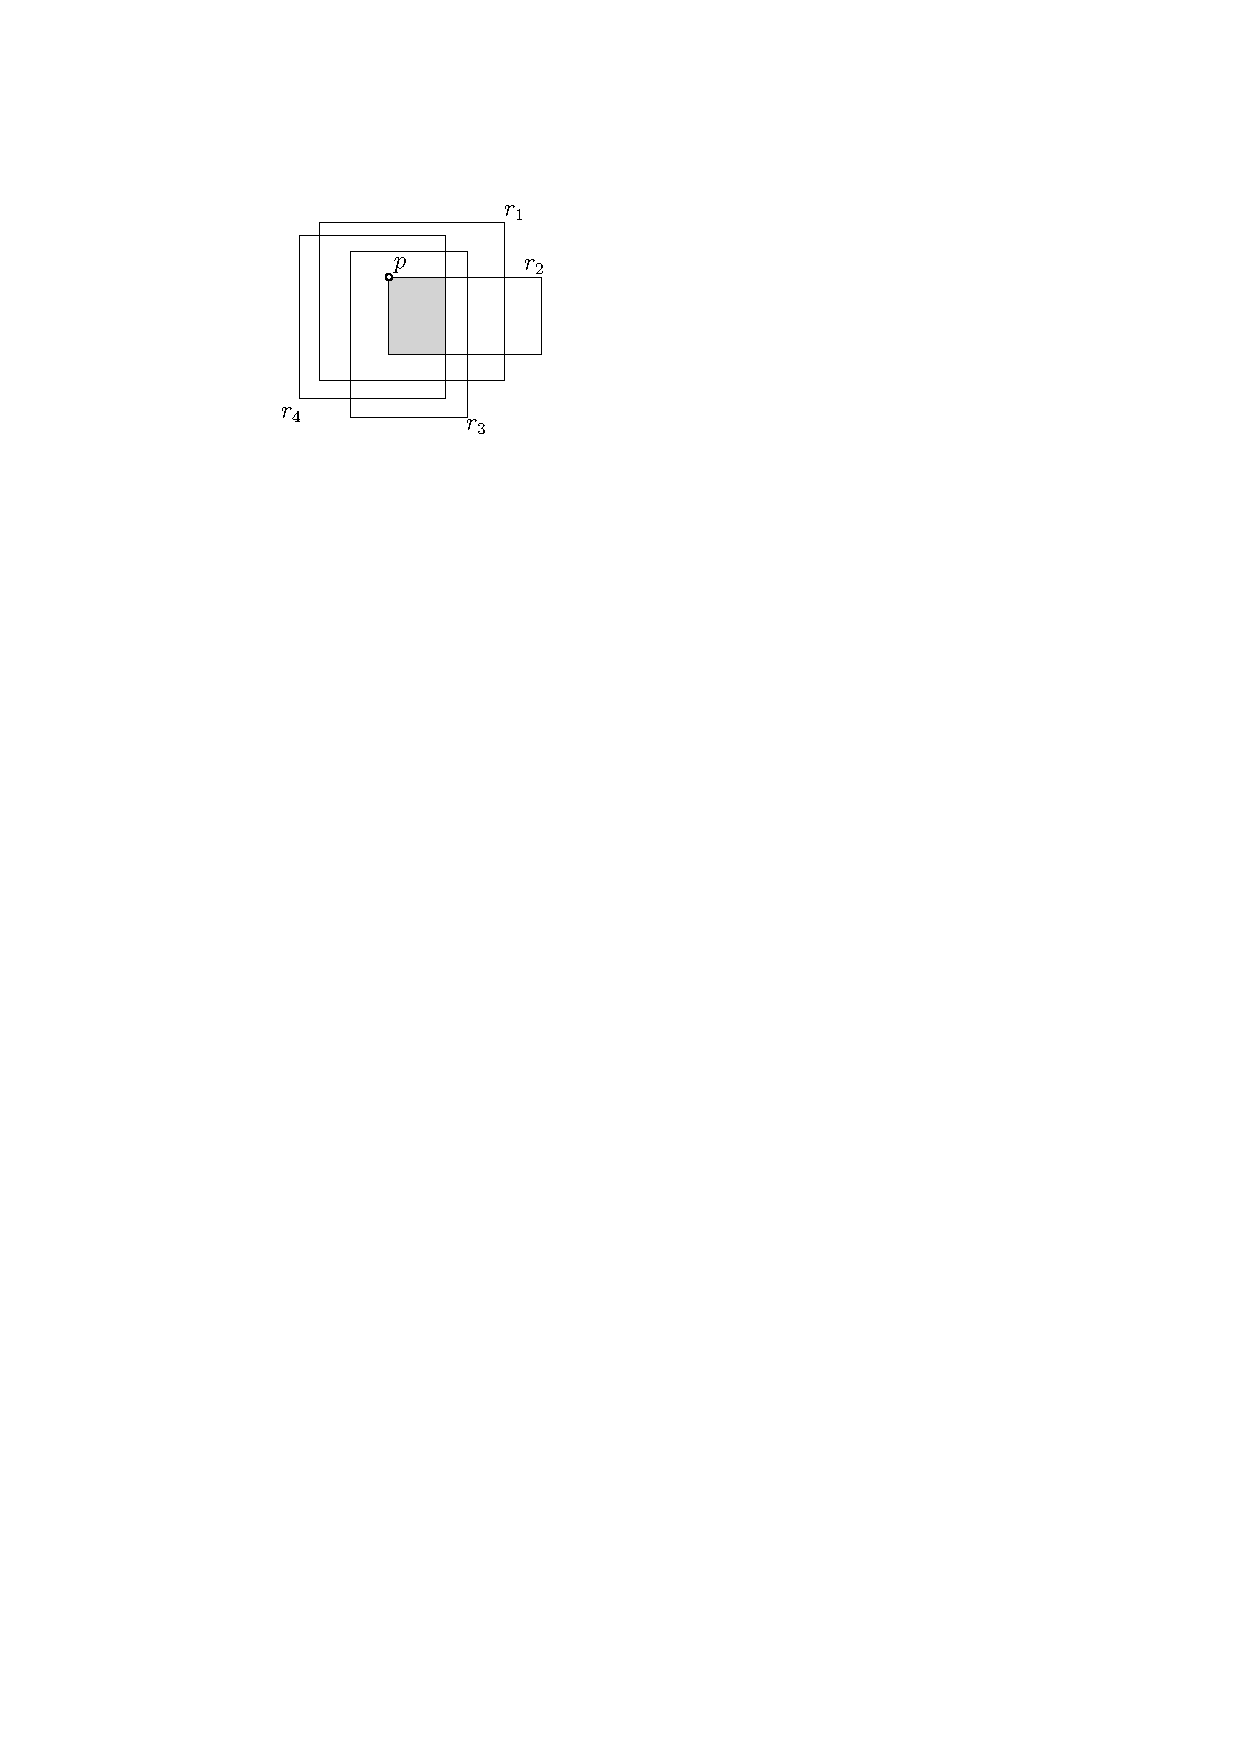
\includegraphics[height=27mm]{./artwork/cat1} &
        \hspace{5mm} 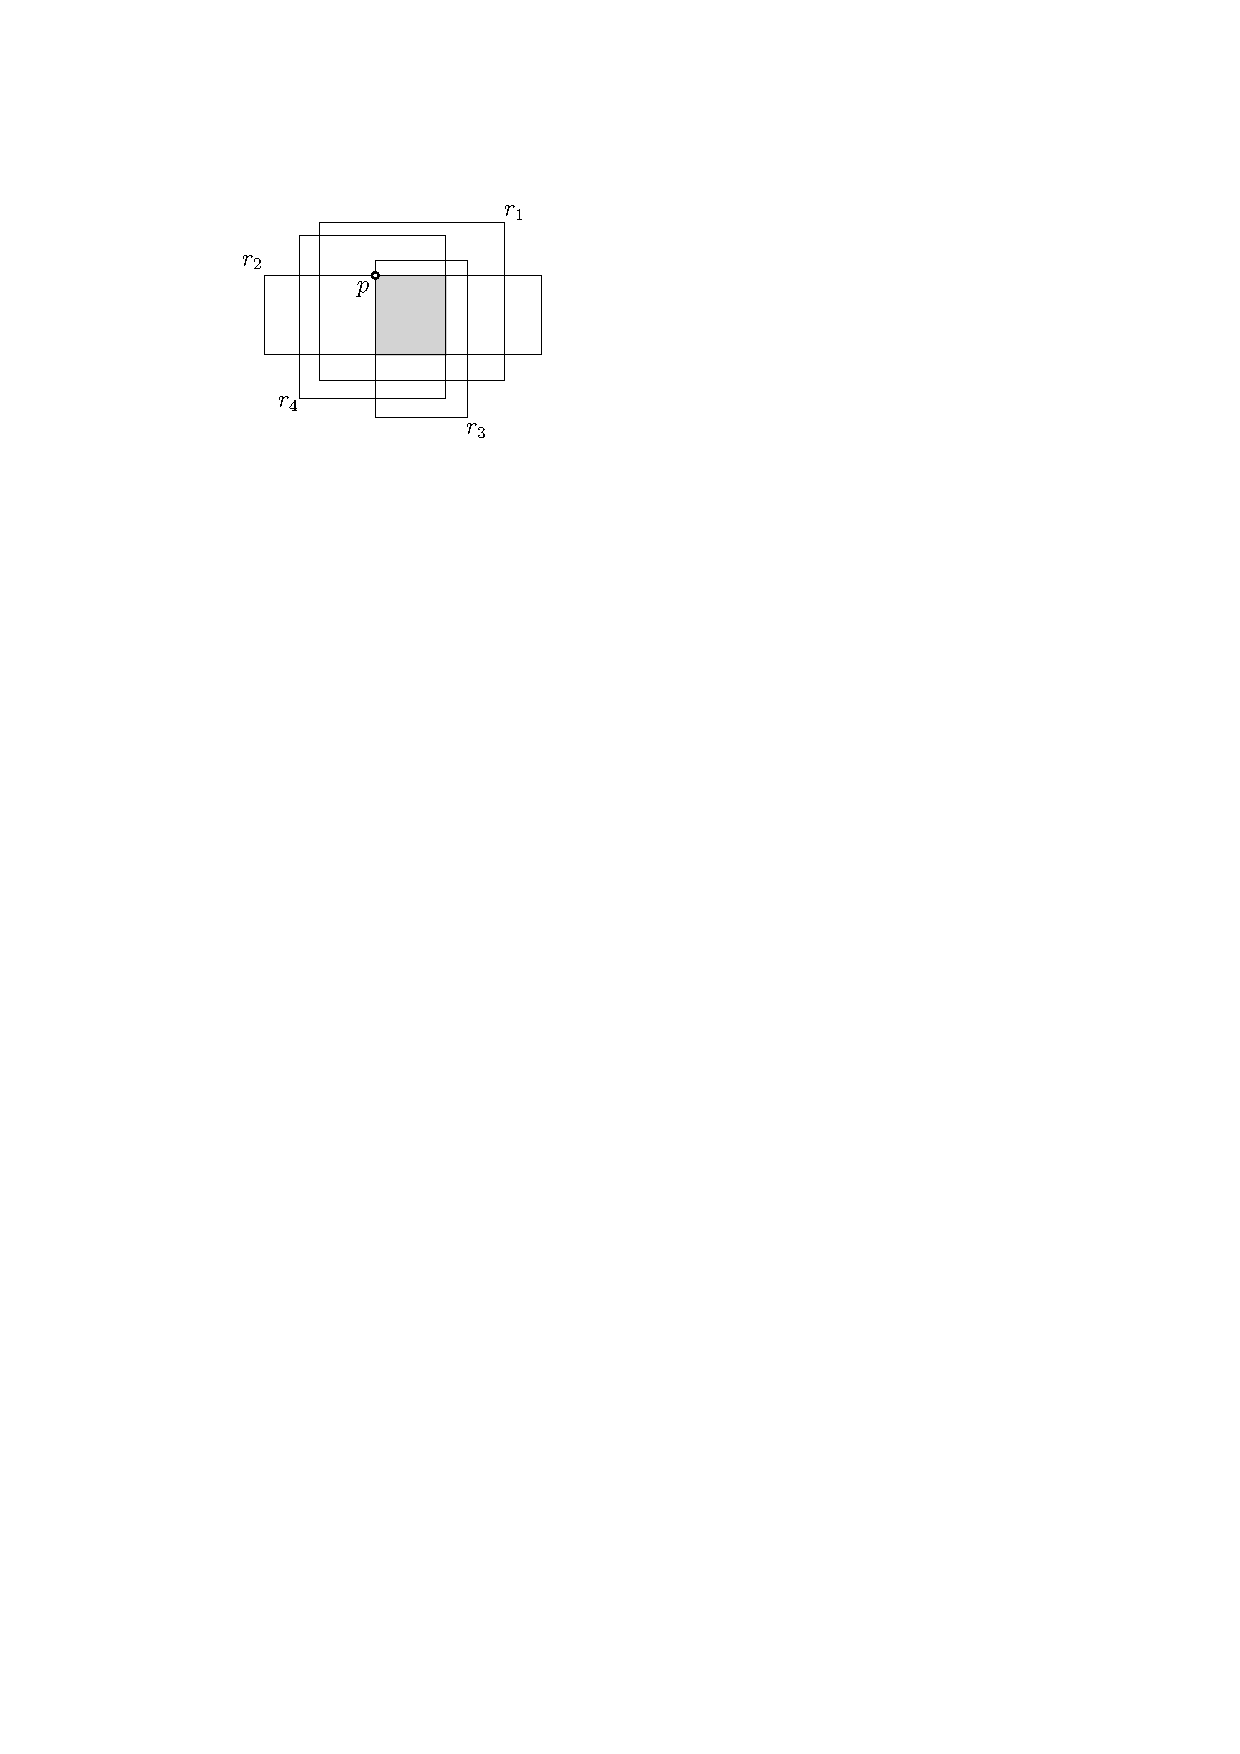
\includegraphics[height=27mm]{./artwork/cat2} \\
        (a) Category 1 &
        (b) Category 2
    \end{tabular}

    \figcapup
    \caption{Classifying $k$-SJ result tuples ($k$ = 4)}
    \label{fig:ksj:cats}
    \figcapdown
\end{figure}

\extraspacing {\bf Category 2.} Given $i, j \in [k]$ with $i \ne j$, we denote by $\J^\catt_{i,j}$ the set of $k$-tuples $\bm{t} = (r_1, ..., r_k) \in \J(R_1, ..., R_k)$ such that the top-left corner of $B_\bm{t}$ is the intersection between the top edge of $r_i$ and the left edge of $r_j$. The Category 2 of result tuples is the union of the $\J^\catt_{i,j}$ of all possible $i, j$. 

\vgap 

The computation of $\J^\catt_{i,j}$ is an instance of the H-V $k$-SJ problem. Specifically, collect the top-edges of all rectangles of $R_i$ into a set $H$, and collect the left-edges of all the rectangles of $R_j$ into a set $V$. This yields an H-V $k$-SJ instance whose input comprises all the $R_z$ with $z \in [k] \setminus \set{i,j}$,  $H$, and $V$. Each result tuple consists of a rectangle $r_z \in R_z$, for $z \in [k] \setminus \set{i,j}$, a horizontal segment $h \in H$, and a vertical segment $v \in V$ such that $h \cap v \cap \bigcap_{z \in [k] \setminus \set{i,j}} r_z \ne \emptyset$. There is one-one correspondence between the output of the H-V $k$-SJ and $\J^\catt_{i,j}$. Thus, by Lemma~\ref{lmm:hv}, the H-V $k$-SJ can be solved in $O(k) \cdot (F_{k-1}(n, |\J^\catt_{i,j}|) + n \log n + k \cdot |\J^\catt_{i,j}|)$ time. Converting the output into $\J^\catt_{i,j}$ takes another $O(|\J^\catt_{i,j}|)$ time. Applying $|\J^\catt_{i,j}| \le \out$, we know that $\J^\catt_{i,j}$ can be produced in $O(k) \cdot (F_{k-1}(n, \out) + n \log n + k \cdot \out)$ time

\vgap 

Performing the above for all $i, j \in [k]$ with $i \ne j$ leads to a total time complexity of $O(k^3) \cdot (F_{k-1}(n, \out) + n \log n + k \cdot \out)$. A category-2 result tuple $\bm{t}$ may be seen more than once (this can happen if, for example, more than one rectangle in $\bm{t}$ has the same top-edge or the same left-edge). Again, duplicate removal can be achieved at no extra cost asymptotically.

\vgap 

We now complete the proof of Theorem~\ref{thm:main-recur}.


\bibliographystyle{plainurl}% the mandatory bibstyle
\bibliography{ref}

\balance

\appendix 

\def\vgap{\vspace{1mm}}

\section*{Appendix}

\section{Building Brick Algorithms} \label{app:bricks}

\extraspacing {\bf Algorithm for Problem $\bm{\mathscr{A}}$.} The {\em interval tree} \cite{bcko08} stores a set $S$ of intervals in $\real$ using $O(|S|)$ space such that, given any real value $q$, the intervals of $S$ containing $q$ can be found in $O(\log |S| + K)$ time, where $K$ is the number of intervals reported. It can also be used to detect whether $S$ has at least one interval containing $q$ in $O(\log |S|)$ time. Each interval insertion or deletion on $S$ can be supported in $O(\log |S|)$ time.

\vgap

Let us first consider the detection version of Problem $\mathscr{A}$. Each point $p = (x, y)$ of $P$ is said to {\em define} the y-coordinate $y$, and each rectangle $r = [x_1, x_2] \times [y_1, y_2]$ of $R$ is said to {\em define} two y-coordinates $y_1$ and $y_2$. We start by sorting the set of y-coordinates defined by all the points and rectangles.

\vgap

Next, sweep (conceptually) a horizontal line $\ell$ from $y = -\infty$ to $y = \infty$. At all times, maintain the set $R_\ell$ of rectangles in $R$ that intersect with $\ell$. Let $S_\ell$ be the set of x-ranges of the rectangles in $R_\ell$; we store $S_\ell$ in an interval tree $\T$. Specifically, when $\ell$ hits the bottom (resp., top) edge of a rectangle $r = [x_1, x_2] \times [y_1, y_2]$ of $R$, we insert (resp., delete) $[x_1, x_2]$ into (resp., from) $\T$, which can be done in $O(\log n)$ time. When $\ell$ hits a point $p = (x, y)$ of $P$, search $\T$ to determine if any interval in $S_\ell$ contains the value $x$. If so, point $p$ is covered by at least one rectangle in $R$; otherwise, it is not. The overall running time is $O(n \log n)$.

\vgap

The algorithm for the reporting version of Problem $\mathscr{A}$ is similar. The only difference is that, when $\ell$ hits a point $p = (x, y)$ of $P$, we use $\T$ to report all the intervals in $S_\ell$ that contain $x$; the cost is $O(n \log n + K_p)$, where $K_p$ is the number of such intervals. Every interval corresponds to a rectangle in $R$ that contains $p$. The total running time is $O(n \log n + \sum_p K_p) = O(n \log n + \out)$.

\extraspacing {\bf Algorithm for Problem $\bm{\mathscr{B}}$.} Each horizontal segment $h = [x_1, x_2] \times y$ of $H$ is said to {\em define} the y-coordinate $y$, and each vertical segment $v = x \times [y_1, y_2]$ of $V$ is said to {\em define} two y-coordinates $y_1$ and $y_2$. We start by sorting the set of y-coordinates defined by all the horizontal and vertical segments.

\vgap

Next, sweep (conceptually) a horizontal line $\ell$ from $y = -\infty$ to $y = \infty$. At all times, maintain the set $V_\ell$ of segments in $V$ that intersect with $\ell$. Let $S_\ell$ be the set of x-coordinates of the segments in $V_\ell$; we store $S_\ell$ in a binary search tree (BST) $\T$. Specifically, when $\ell$ hits the lower  (resp., upper) endpoint of a vertical segment $v = x \times [y_1, y_2]$ of $V$, we insert (resp., delete) the value $x$ into (resp., from) $\T$, which can be done in $O(\log n)$ amortized time. When $\ell$ hits a horizontal segment $h = [x_1, x_2] \times y$ of $H$, search $\T$ to determine if the successor $x'$ of $x_1$ in $S_\ell$. If $x' \le x_2$, then we output a pair $(h, p)$, where $p$ is the point $(x', y)$. The overall running time is $O(n \log n)$.

\extraspacing {\bf Algorithm for Problem $\bm{\mathscr{C}}$.} Let $S$ be a set of intervals in $\real$, each of which is associated with a real-valued {\em weight}. Given a real value $q$, a {\em stabbing max} query returns the maximum weight of all the intervals in $S$ covering $q$ (if no such intervals exist, the query returns $-\infty$). We can store $S$ in a structure of \cite{aak+12} using $O(|S|)$ space that can answer every query in $O(\log |S|)$ time. The structure also supports an insertion or deletion on $S$ in $O(\log |S|)$ amortized time.

\vgap

For Problem $\mathscr{C}$, each horizontal segment $h = [x_1, x_2] \times y$ of $H$ is said to {\em define} the y-coordinate $y$, and each rectangle $r = [x_1, x_2] \times [y_1, y_2]$ of $R$ is said to {\em define} two y-coordinates $y_1$ and $y_2$. We start by sorting the set of y-coordinates defined by all the horizontal segments and rectangles.

\vgap

Next, sweep (conceptually) a horizontal line $\ell$ from $y = -\infty$ to $y = \infty$. At all times, maintain the set $R_\ell$ of rectangles in $R$ that intersect with $\ell$. Let $S_\ell$ be the set of x-ranges of the rectangles in $R_\ell$; we store $S_\ell$ in a structure $\T$ of \cite{aak+12}. Specifically, when $\ell$ hits the bottom (resp., top) edge of a rectangle $r = [x_1, x_2] \times [y_1, y_2]$ of $R$, we insert (resp., delete) $[x_1, x_2]$ with {\em weight} $x_2$ into (resp., from) $\T$, which can be done in $O(\log n)$ time. When $\ell$ hits a horizontal segment $h = [x_1, x_2] \times y$ of $P$, search $\T$ to determine the maximum weight $w$ of all the intervals in $S_\ell$ containing the value $x_1$. If $w \ne -\infty$, we output $(h, p)$ where the point $p$ is defined in a way depending on $w$: if $w \le x_2$, then $p = (w, y)$; otherwise $p = (x_2, y)$. The overall running time is $O(n \log n)$.

\extraspacing {\bf Algorithm for Problem $\bm{\mathscr{D}}$.} The {\em priority search tree} (PST) \cite{m85} stores a set $P$ of points using $O(|P|)$ space such that, given any 3-sided rectangle $q = [x_1, x_2] \times [y, \infty)$, the points of $S$ covered by $q$ can be found in $O(\log |P| + K)$ time, where $K$ is the number of points reported. This structure can be used to answer the following {\em containment query} on intervals: store a set $S$ of intervals in $\real$ using $O(|S|)$ space such that, given any interval $q' = [z_1, z_2]$, the intervals of $S$ that are contained in $q'$ can be found in $O(\log |S| + K)$ time, where $K$ is the number of intervals reported. To see why, observe that an interval $[z_1, z_2]$ contains another $[x, y]$ if and only if the point $(x, y)$ is covered by the 3-sided rectangle $[z_1, \infty) \times (-\infty, z_2]$. Thus, we can create from $S$ a set of points $P = \set{(x, y) \mid [x, y] \in S}$ and store $P$ in a PST. Given an interval $q' = [z_1, z_2]$, we use the PST to find all the points in $P$ covered by $q = [z_1, \infty) \times (-\infty, z_2]$ and, for each such point $(x, y)$, report $[x, y]$.

%\vgap

%A PST built on a set $P$ of points can also answer the following detection query in $O(\log |P|)$ time: given any 3-sided rectangle $q = [x_1, x_2] \times [y, \infty)$, decide whether $P$ contains at least one point covered by $q$. Accordingly, a PST built on a set $S$ of intervals can also answer the detection version of the containment query in $O(\log |S|)$ time: specifically, given any interval $q' = [z_1, z_2]$, decide whether $S$ has at least one interval that is contained in $q'$.

\vgap

Let us now return to the context of $\mathscr{D}$. We assume, w.l.o.g., that each rectangle of $R$ is given a distinct ID in $[n]$. Let us first consider the detection version. Initialize an array $A$ of size $|R|$, where cell $A[i]$, $i \in [|R|]$, is allocated to the rectangle $r$ with ID $i$ and will be used to store a constant amount of information for $r$. In the outset, all rectangles of $R$ are marked as inactive (in $A$). During our algorithm, the status of each rectangle will turn from inactive to active at some point, turn from active back to inactive at a later point, and then stay that way forever.

\vgap

Sweep (conceptually) a horizontal line $\ell$ from $y = -\infty$ to $y = \infty$. At all times, we maintain the set $R_\ell$ of {\em active} rectangles in $R$ that intersect with $\ell$. Let $S_\ell$ be the set of x-ranges of the rectangles in $R_\ell$; we store $S_\ell$ in a PST $\T$. Specifically, when $\ell$ hits the bottom edge of a rectangle $r = [x_1, x_2] \times [y_1, y_2]$ of $R$, we insert $[x_1, x_2]$ into $\T$ and mark $r$ as active, which can be done in $O(\log n)$ time. The rectangle $r$ will be referred to as the {\em host} of $[x_1, x_2]$ and is stored together with $[x_1, x_2]$ in $\T$.

\vgap

When $\ell$ hits a horizontal segment $h = [z_1, z_2] \times y$ of $P$, perform a containment query on $\T$ to find all the intervals in $S_\ell$ that are contained by $[z_1, z_2]$; if $K_h$ is the number of such intervals, this retrieval takes $O(\log n + K_h)$ time. For each retrieved interval $[x_1, x_2]$, we also obtain its host rectangle $r$ (stored along with $[x_1, x_2]$ in $\T$). Observe that $h$ is the lowest segment in $H$ that crosses $r$. We store $h$ in the cell of array $A$ allocated to $r$, after which $r$ is marked as inactive, and accordingly, its x-range $[x_1, x_2]$ is deleted from $T$ in $O(\log n)$ time. As $r$ will remain inactive in the rest of the execution, its x-range will not be retrieved again by another containment query in the future.

\vgap

When $\ell$ hits the bottom edge of a rectangle $r = [x_1, x_2] \times [y_1, y_2]$ of $R$, we check whether $r$ is active. If so, delete $[x_1, x_2]$ from $\T$ and mark $r$ as inactive; otherwise, do nothing.

\vgap

Overall, each rectangle of $R$ necessitates one insertion and one deletion in $\T$. All these insertions and deletions take $O(n \log n)$ time in total. Each segment $h$ of $H$ performs a containment query on $\T$, which has a cost of $O(\log n + K_h)$. All these queries demand a total cost of $O(n \log n + \sum_h K_h)$. Recall that the x-range of a rectangle in $R$ can be retrieved by at most one containment query. Hence, $\sum_h K_h \le n$ and the runtime of our algorithm is $O(n \log n)$.

\vgap

Next, we consider the find-all-sorted version of Problem $\mathscr{D}$. Again, initialize an array $A$ of size $|R|$, where each rectangle of $R$ is allocated a cell. For each $r \in R$, we keep a linked list, which at the end of our algorithm will store the horizontal segments of $\cross_H(r)$ in ascending order of their y-coordinates. A pointer referencing the linked list is stored in the cell of $A$ allocated to $r$. In the outset, all linked lists are empty. Unlike the detection version, we will not need to keep the active status for the rectangles.

\vgap

Again, sweep a horizontal line $\ell$ from $y = -\infty$ to $y = \infty$. At all times, we maintain the set $R_\ell$ of rectangles in $R$ that intersect with $\ell$. Let $S_\ell$ be the set of x-ranges of the rectangles in $R_\ell$; we store $S_\ell$ in a PST $\T$. Specifically, when $\ell$ hits the bottom (resp., top) edge of a rectangle $r = [x_1, x_2] \times [y_1, y_2]$ of $R$, we insert (resp., delete) $[x_1, x_2]$ into (resp., from) $\T$, which can be done in $O(\log n)$ time. Again, the rectangle $r$ --- the host of $[x_1, x_2]$ --- is stored together with $[x_1, x_2]$ in $\T$.

\vgap

When $\ell$ hits a horizontal segment $h = [z_1, z_2] \times y$ of $P$, perform a containment query on $\T$ to find all the intervals in $S_\ell$ that are contained by $[z_1, z_2]$; the query cost is $O(\log n + K_h)$, where $K_h$ is the number of intervals reported. For each retrieved interval $[x_1, x_2]$, we also obtain its host rectangle $r$. It is clear that $h$ is a segment crossing $r$ and is thus appended to the linked list of $r$. Note that $h$ is higher than all the segments already in that linked list.

\vgap

Overall, each rectangle of $R$ necessitates one insertion and one deletion in $\T$. All these insertions and deletions take $O(n \log n)$ time in total. Each segment $h$ of $H$ performs a containment query on $\T$, which has a cost of $O(\log n + K_h)$. All these queries demand a total cost of $O(n \log n + \sum_h K_h)$. However, unlike the detection version, the sum $\sum_h K_h$ here is equal to the total size of $\cross_H(r)$ for all the $r \in R$. The total size is equivalent to $\out$.


\extraspacing {\bf Algorithm for Problem $\bm{\mathscr{E}}$.}


\section{Completing the Proof of Lemma~\ref{lmm:hv}} \label{app:hv} 

\extraspacing {\bf Proof of Lemma~\ref{lmm:hv:type1:recur-output}.} We will prove the lemma by providing a way to map each $(k-2)$-tuple $\J(R_1',...,R_{k-2}')$ to a unique $k$-tuple in the H-V $k$-SJ result $\J(R_1,...,R_{k-2},H,V)$.

\vgap

To explain the mapping, consider any tuple $\bm{t} \in \J(R_1',...,R_{k-2}')$. Recall that $B_\bm{t}$ is the intersection of the $k-2$ rectangles $\bm{t}[1], ..., \bm{t}[k-2]$. Let $p$ be the bottom-left corner of $B_\bm{t}$. Define $i$ and $j$ to be values in $[k-2]$ such that $\bm{t}[i] = \gbot(\bm{t})$ and $\bm{t}[j] = \gleft(\bm{t})$; note that $i$ and $j$ can be the same. Point $p$ is the intersection of the bottom edge of $\bm{t}[i]$ and the left edge of $\bm{t}[j]$.

\vgap

Recall that each $\bm{t}[z]$ (for $z \in [k-2]$) is a trimmed rectangle; let us denote by $r_z$ the full rectangle of $\bm{t}[z]$. Regarding the values $i, j$ decided earlier, let
\myitems{
    \item $h$ be the lowest segment in $H$ that crosses $r_i$;
    \item $v$ be the leftmost segment in $V$ that crosses $r_j$.
}
By the way trimmed rectangles are computed, we know that $h$ must contain the bottom edge of rectangle $\bm{t}[i]$, and $v$ must contain the left edge of rectangle $\bm{t}[j]$. This means that point $p$ must be the intersection point of $h$ and $v$.

\vgap

We argue that the $k$-tuple $(r_1, ..., r_{k-2}, h, v)$ belongs to $\J(R_1,...,$ $R_{k-2},H,V)$. Clearly, $r_z$ covers $\bm{t}[z]$ for all $z \in [k-2]$. Thus, $\bigcap_{z=1}^{k-2} r_z$ covers $\bigcap_{z=1}^{k-2} \bm{t}[z]$, which is $B_\bm{t}$. Hence, point $p$ --- which is the intersection point of $h$ and $v$, and also a corner of $B_\bm{t}$ --- falls in $\bigcap_{z=1}^{k-2} r_z$, indicating $h \cap v \cap \bigcap_{z=1}^{k-2} r_z \ne \emptyset$. We map $\bm{t}$ to $(r_1, ..., r_{k-2}, h, v)$.

\vgap

It remains to prove that no two distinct tuples $\bm{t}_1, \bm{t}_2 \in \J(R_1',...,$ $R_{k-2}')$ can be mapped to the same tuple in $\J(R_1,..., R_{k-2},$ $H, V)$. Assume that this is not true, namely, both $\bm{t}_1$ and $\bm{t}_2$ are mapped to $(r_1, ..., r_{k-2}, h, v) \in \J(R_1,..., R_{k-2}, H, V)$. However, in this case, $\bm{t}_1[z]$ is the trimmed rectangle of $r_z$ for all $z \in [k-2]$ and, at the same time, $\bm{t}_2[z]$ is the trimmed rectangle of $r_z$ for all $z \in [k-2]$. We thus have $\bm{t}_1 = \bm{t}_2$, giving a contradiction.

\extraspacing {\bf Proof of Lemma~\ref{lmm:hv:type1:properties}.} \\
\underline{\em Proof of Statement (1).} As $h \in \dcross_H(\bm{t})$ and $v \in \dcross_V(\bm{t})$, the two segments both cross $B_\bm{t}$, as can be verified from the definitions of $\dcross_H(\bm{t})$ and $\dcross_V(\bm{t})$. Thus, the intersection of $h$ and $v$ is a point $p$ in $B_\bm{t}$. As $r_i$ (for each $i \in [k-2]$) is the full rectangle of $\bm{t}[i]$, we know that $\bigcap_{i=1}^{k-2} r_i$ covers $B_\bm{t} = \bigcap_{i=1}^{k-2} \bm{t}[i]$. Hence, point $p$ falls in $\bigcap_{i=1}^{k-2} r_i$, indicating that $h\cap v \cap \bigcap_{i = 1}^{k-2}r_i \neq \emptyset$. It follows that $(r_1,...,r_{k-2},h,v)$ is a result tuple in $\J(R_1,...,R_{k-2},H,V)$.

\vgap

\noindent \underline{\em Proof of Statement (2).} Fix any rectangle $r \in R_1 \cup ... \cup R_{k-2}$ and any horizontal segment $h = [x_1, x_2] \times y$ from $H$ that crosses $r$. We will show that $h$ must also cross the trimmed rectangle $r'$ of $r$. From the fact of $h$ crossing $r$, it is clear that $[x_1, x_2]$ contains the x-range of $r$. As the x-range of $r$ contains that of $r'$, we can assert that $[x_1, x_2]$ contains the x-range of $r'$. To prove that $h$ crosses $r'$, we still need to show $y \in [\ybot(r'), \ytop(r')]$. Recall that $\ybot(r')$ is the y-coordinate of the lowest segment in $H$ crossing $r$. This implies $y \ge \ybot(r')$ because $h$ itself is a segment in $H$ crossing $r$. Analogously, it also holds that $y \le \ytop(r')$. We can thus conclude that $h$ crosses $r'$. 

\vgap

Fix any rectangle $r \in R_1 \cup ... \cup R_{k-2}$ and any vertical segment $v$ from $V$ that crosses $r$. An argument symmetric to the above shows that $v$ must also cross the trimmed rectangle $r'$.

\vgap

We now prove the first bullet of statement (2), namely, $\bm{t}\in \J(R_1',...,R_{k-2}')$. Consider the $k$-tuple $(r_1,...,r_{k-2},h,v)\in \J_1$ given in statement (2). By definition of $\J_1$, segments $h$ and $v$ both cross each of the rectangles $r_1,..., r_{k-2}$. By the earlier discussion, $h$ and $v$ must also cross each of the trimmed rectangles $r_1',..., r_{k-2}'$. Hence, the intersection of $h$ and $v$ must be a point covered by each of $r_1',..., r_{k-2}'$. This suggests that the point is in $\bigcap_{i = 1}^{k-2}r_i'$, which thus cannot be empty. Therefore, $\bm{t} = (r_1', ..., r_{k-2}')$ is a result tuple in $\J(R_1',...,R_{k-2}')$. 

\vgap 

Next, we prove the second bullet, namely, $h \in \dcross_H(\bm{t})$ and $v \in \dcross_V(\bm{t})$. It suffices to show only the former due to symmetry. To prove $h \in \dcross_H(\bm{t})$, we need to argue that $h$ crosses $\gbot(\bm{t})$ and $B_\bm{t}$. The first part, $h$ crossing $\gbot(\bm{t})$, is done because, as already explained, $h$ crosses each of $r_1', ..., r_{k-2}'$, and $\gbot(\bm{t})$ is one of those $k-2$ rectangles. To prove that $h$ crosses $B_\bm{t}$, first note that $B_\bm{t}$ (which is the intersection of $r_1', ..., r_{k-2}'$) is covered by $\gbot(\bm{t})$. The fact that $h$ crosses $\gbot(\bm{t})$ indicates that the y-range of $h$ contains that of $B_\bm{t}$. Hence, either $h$ is disjoint with $B_\bm{t}$ or $h$ crosses $B_\bm{t}$. However, $h$ cannot be disjoint with $B_\bm{t}$ because, as shown earlier, the intersection of $h$ and $v$ falls in $B_\bm{t}$. It thus follows that $h$ crosses $B_\bm{t}$.

\vgap 

\noindent \underline{\em Proof of Statement (3).} We first prove that $\dcross_H(\bm{t}) \neq \emptyset$ for any $\bm{t} \in \J(R_1',...,R_{k-2}')$. Set $r' = \gbot(\bm{t})$, and let $r$ be the full rectangle of $r'$. Define $h$ as the lowest segment crossing $r$ (note that $h$ definitely exists because otherwise $r$ has no trimmed rectangle). We will show that $h \in \dcross_H(\bm{t})$, and hence $\dcross_H(\bm{t})$ cannot be empty. For this purpose, we should explain why $h$ crosses both $B_{\bm{t}}$ and $r'$. However, $h$ crossing $r$ implies $h$ crossing $r'$, as has already been argued in our proof of statement (2). It remains to show that $h$ crosses $B_\bm{t}$.

\vgap

By the way $r'$ is defined, the bottom edge of $r'$ must be contained in $h$. Because $r' = \gbot(\bm{t})$, the bottom edge of $B_\bm{t}$ is contained in the bottom edge of $r'$ and hence also contained in $h$. This means that $h \cap B_{\bm{t}}\neq \emptyset$. On the other hand, the x-range of $h$ must contain that of $r'$ (because $h$ crosses $r'$), which in turn must contain that of $B_\bm{t}$ (because $r'$ covers $B_\bm{t}$). Thus, the x-range of $h$ covers that of $B_\bm{t}$. Combining this with $h \cap B_{\bm{t}}\neq \emptyset$ yields that $h$ must cross $B_\bm{t}$.

\vgap 

A symmetric argument assures us that $\dcross_V(\bm{t}) \ne \emptyset$ for any $\bm{t} \in \J(R_1',...,R_{k-2}')$. 

%In other words, both $\dcross_H(\bm{t})$ and $\dcross_V(\bm{t})$ must have size at least 1.

\vgap 

Next, we will prove 
\myeqn{
    \sum_{\bm{t}\in \J(R_1',...,R_{k-2}')} |\dcross_H(\bm{t})| \cdot |\dcross_V(\bm{t})| \leq \out. \label{eqn:hv:type1:properties:proof-help1}
} 
which implies statement (3) because, for any $\bm{t}$ in the summation, $|\dcross_H(\bm{t})| \ge 1$ and $|\dcross_V(\bm{t})| \ge 1$. Our proof resorts to the algorithm generate-$\J^*$ (see Section~\ref{sec:hv:type1}). This algorithm adds to $\J^*$ exactly as many tuples as calculated by the left hand side of \eqref{eqn:hv:type1:properties:proof-help1}. By statement (2), the $\J^*$ produced must be a subset of $\J(R_1,...,R_{k-2},H,V)$, whose size is $\out$. This establishes the inequality in \eqref{eqn:hv:type1:properties:proof-help1}, which completes the proof of statement (3).

\extraspacing {\bf Proof of Lemma~\ref{lmm:hv:type1:cross-r*}.} \\
\underline{\em Proof of Statement (1).} We will map each $r^*\in \bigcup_{i = 1}^{k-2} R_i^*$ to a unique tuple $\bm{t}\in \J(R_1',...,R_{k-2}')$ satisfying $\dcross_H(\bm{t}) = \cross_H(r^*)$. After this, we can then derive $\sum_{i\in[k-2]}\sum_{r^*\in R_i^*} |\cross_H(r^*)| \leq \sum_{\bm{t}\in \J(R_1',...,R_{k-2}')}|\dcross_H(\bm{t})|\leq \out$, where the last step used  statement (3) of Lemma~\ref{lmm:hv:type1:properties}.

\vgap

The mapping is designed as follows. Consider an arbitrary $r^*\in \bigcup_{i = 1}^{k-2} R_i^*$. Recall that $r^*$ is the top-sliced of some rectangle $r'$. Specifically, if $r' = [x_1,x_2]\times [y_1,y_2]$, then $r^* = [x_1,x_2]\times [y_1,\maxtop(r')]$. By the definition of $\maxtop(r')$ in \eqref{eqn:hv:type1:topsliced}, there exists a tuple $\bm{t}\in \J(R_1',...,R_{k-2}')$ satisfying $\gbot(\bm{t}) = r'$ and $\maxtop(r') = \ytop(B_{\bm{t}})$. We map $r^*$ to $\bm{t}$.

\vgap

Next, we will prove that a segment $h \in \cross_H(r^*)$ if and only if $h \in \dcross_H(\bm{t})$. Let us start with the ``only-if direction'': assuming $h \in \cross_H(r^*)$, we aim to show $h \in \dcross_H(\bm{t})$. For this purpose, we need to show that $h$ crosses both $\gbot(\bm{t}) = r'$ and $B_\bm{t}$.
\myitems {
    \item First, we explain why $h$ crosses $r'$. Because $r'$ covers $r^*$, by the fact $h$ crossing $r^*$, we know that $h$ must intersect with $r'$. On the other hand, as $h$ crosses $r^*$, it must hold that $\xleft(h) < x_1 \le x_2 < \xright(h)$ (recall that $[x_1, x_2]$ is the x-range of $r^*$). As $[x_1, x_2]$ is also the x-range of $r'$, using the fact of $h \cap r' \ne \emptyset$, we can assert that $h$ crosses $r'$.

    \vgap

    \item Then, we explain why $h$ crosses $B_{\bm{t}}$. Note that because $h$ crosses $r'$ (which we just proved) and $B_{\bm{t}}\subseteq r'$, we know that $B_{\bm{t}}$ cannot contain any endpoint of $h$. Let $y_h$ be the y-coordinate of $h$, and take the point $p = (\xleft(B_{\bm{t}}), y_h)$. We will prove $p \in h \cap B_{\bm{t}}$, suggesting $h\cap B_{\bm{t}} \neq \emptyset$ and, hence, $h$ must cross $B_{\bm{t}}$ (because no endpoint of $h$ falls in $B_\bm{t}$, as mentioned).

    \vgap

    Since $\gbot(\bm{t}) = r'$, the bottom edge of $B_{\bm{t}}$ must be contained in $r'$. Thus, $\xleft(B_{\bm{t}})\in [x_1,x_2]$. As proved earlier, $\xleft(h) < x_1 \le x_2 < \xright(h)$, which leads to $\xleft(B_{\bm{t}}) \in [\xleft(h), \xright(h)]$, suggesting $p \in h$.

    \vgap

    Because $\gbot(\bm{t}) = r'$ and $\maxtop(r') = \ytop(B_\bm{t})$, the y-range of $B_\bm{t}$ is $[y_1, \maxtop(r')]$. To prove $p \in B_{\bm{t}}$, it remains to show $y_h \in [y_1, \maxtop(r')]$. This is true because $h$ intersects $r^*$ and $[y_1, \maxtop(r')]$ is the y-range of $r^*$.
}

Our argument now proceeds to prove the ``if direction'': assuming $h \in \dcross_H(\bm{t})$, we aim to show $h \in \cross_H(r^*)$. Recall that $r^* = [x_1,x_2] \times [y_1, \maxtop(r')]$. To prove that $h$ crosses $r^*$, we will show $\xleft(h) < x_1 \le x_2 < \xright(h)$ and $y_h \in [y_1, \maxtop(r')]$, where $y_h$ is the y-coordinate of $h$.
\myitems{
    \item The fact $h \in \dcross_H(\bm{t})$ tells us that $h$ crosses $r'$. As $[x_1, x_2]$ is the x-range of $r'$, we know $\xleft(h) < x_1 \le x_2 < \xright(h)$.

    \vgap

    \item The fact $h \in \dcross_H(\bm{t})$ also tells us that $h$ crosses $B_{\bm{t}}$. As $[y_1, \maxtop(r')]$ is the y-range of $B_\bm{t}$ (because $\gbot(\bm{t}) = r'$ and $\maxtop(r') = \ytop(B_\bm{t})$), we know $y_h \in [y_1, \maxtop(r')]$.
}

It remains to show that no two distinct rectangles $r_1^*, r_2^* \in \bigcup_{i = 1}^{k-2}R_i^*$ can be mapped to the same tuple in $\J(R_1',...,R_{k-2}')$. Assume, on the contrary, that $r_1^*$ and $r_2^*$ are mapped to the same tuple $\bm{t}\in \J(R_1',...,R_{k-2}')$. Suppose that $r_1^*$ (resp., $r_2^*$) is the top-sliced rectangle of $r_1'$ (resp., $r_2'$). Under our mapping, it must be true that  $r_1' = r_2' = \gbot(B_{\bm{t}})$. However, the distinctness of $r_1^*$ and $r_2^*$ requires $r_1' \ne r_2'$, thus giving a contradiction.

\extraspacing \underline{\em Proof of Statement (2).}
Let $r', r^*$, and $\bm{t}$ be as defined in statement (2). Let us represent $r'$ as $[x_1,x_2] \times [y_1, y_2]$. Accordingly, $r^*$ can be written as $[x_1, x_2] \times [y_1, \maxtop(r')]$.

\vgap

We will first prove $\dcross_H(\bm{t})\subseteq \cross_H(r^*)$. For this purpose, given any segment $h \in \dcross_H(\bm{t})$, we will show that $h$ crosses $r^*$. To do so, we need to explain why $\xleft(h) < x_1 \le x_2 < \xright(h)$ and $y_h \in [y_1, \maxtop(r')]$.
\begin{itemize}
    \item The fact $h \in \dcross_H(\bm{t})$ tells us that $h$ crosses $\gbot(\bm{t})$, which is $r'$. As the x-range of $r'$ is $[x_1,x_2]$, it must hold true that $\xleft(h) < x_1 \le x_2 < \xright(h)$.

    \vgap

    \item The fact $h \in \dcross_H(\bm{t})$ also tells us that $h$ crosses $B_{\bm{t}}$. Hence, $y_h \in [\ybot(B_\bm{t}), \ytop(B_{\bm{t}})]$. From $r' = \gbot(\bm{t})$, we get $\ybot(B_\bm{t}) = \ybot(r') = y_1$. By the definition of $\maxtop(r')$ in \eqref{eqn:hv:type1:maxtop}, we know $\ytop(B_{\bm{t}}) \leq \maxtop(r')$. It thus follows that $y_h \in [y_1, \maxtop(r')]$.
\end{itemize}
We can now conclude that $h$ crosses $r^*$.

\vgap

Next, assuming that the segments of $\cross_H(r^*)$ are sorted in ascending order of their y-coordinates,
we will prove that $\dcross_H(\bm{t})$ includes a prefix of the sorted order. It suffices to establish the following equivalent statement:

\vgap

\minipg{0.8\linewidth} {
    If a segment $h \in \cross_H(r^*)$ has y-coordinate $y_h \le \ytop(B_{\bm{t}})$, then $h$ must be in $\dcross_H(\bm{t})$.
}

\vgap

\noindent To prove the above, we must explain why $h$ crosses both $r'$ and $B_{\bm{t}}$.

\vgap

We first show that $h$ crosses $r'$, or equivalently: $\xleft(h)  < x_1 \leq x_2 < \xright(h)$ and $y_h \in [y_1, y_2]$. These conditions hold true because $h$ crosses $r^* = [x_1,x_2]\times [y_1, \maxtop(r')]$, and $\maxtop(r')\leq y_2$ (due to the definition of top-sliced rectangle in \eqref{eqn:hv:type1:topsliced}).

\vgap

Finally, we show that $h$ crosses $B_{\bm{t}}$, or equivalently: $\xleft(h) < \xleft(B_{\bm{t}}) \le \xright(B_{\bm{t}}) < \xright(h)$ and $y_h \in [\ybot(B_\bm{t}), \ytop(B_{\bm{t}})] = [y_1, \ytop(B_{\bm{t}})]$.
\begin{itemize}
    \item The fact of $h$ crossing $r'$ tells us $\xleft(h) < x_1 \leq x_2 < \xright(h)$. As $r' = \gbot(B_{\bm{t}})$, the x-range of $B_{\bm{t}}$ must be contained in $[x_1,x_2]$. Therefore, $\xleft(h) < \xleft(B_{\bm{t}}) \le \xright(B_{\bm{t}}) < \xright(h)$.

    \vgap

    \item The fact of $h$ crossing $r^*$ also tells us that $y_h \in [y_1, \maxtop(r')]$. Moreover, by the definition of $h$, we have $y_h \leq \ytop(B_{\bm{t}})$. It thus follows that $y_h \in [y_1, \ytop(B_{\bm{t}})]$.
\end{itemize}


\extraspacing {\bf Proof of Lemma~\ref{lmm:hv:type2:recur-output}.}

We prove by mapping each tuple $\J(R_1,...,R_{k-3},H',V)$ to a unique tuple in $\J_2$. 
To define the mapping, consider an arbitrary tuple $(r_1,...,r_{k-3}, h', v) \in \J(R_1,...,R_{k-3},H',V)$. Let $h$ be the full segment of $h'$. By the definition of the trimmed segment (see Section~\ref{sec:hv:type2}), there exists a rectangle $r_{k-2}\in R_{k-2}$ that covers the right endpoint of $h'$, and the left endpoint of $h$, which is the same as the left endpoint of $h'$. In another word, $r_{k-2}$ covers $h'$. Let $\bm{t} = (r_1,...,r_{k-3}, r_{k-2},h,v)$. We map the tuple $(r_1,...,r_{k-3}, h', v)$ to $\bm{t}$. 

\vgap 

We argue that $\bm{t}\in \J_2$. Let $p$ be the intersection point of $h'$ and $v$. As $h' \subseteq h$, the point $h\cap v$ is the same as $p$.
Since $(r_1,...,r_{k-3}, h', v) \in \J(R_1,...,R_{k-3},H',V)$, $p \in r_i$ for $i \in [k-3]$. As shown in the last paragraph, $r_{k-2}$ covers $h'$, so $p \in r_{k-2}$. Thus, $h \cap v \bigcap_{i = 1}^{k-2}r_i \neq \emptyset$, and $\bm{t} \in \J(R_1,...,R_{k-2},H,V)$.
 Additionally, by the definiton of $r_{k-2}$ in the last paragraph, $r_{k-2}$ covers the left endpoint of $h$. Therefore, $\bm{t} \in \J_2$.

\vgap

It remains to prove that no two distinct tuple $\bm{t}_1, \bm{t}_2$ will be mapped to the same tuple in $\J_2$. Assume, on the contrary, $\bm{t}_1, \bm{t}_2$ are mapped to the same tuple $\bm{t} \in \J_2$. Then, $\bm{t}_1[i] = \bm{t}[i] = \bm{t}_2[i]$ for each $i\in [k-3]$ and $i = k-1$. Moreover, $\bm{t}_1[k-2]$ and $\bm{t}_2[k-2]$ are both the trimmed segment of $\bm{t}[k-2]$. By the uniqueness of the trimmed segment, $\bm{t}_1[k-2] = \bm{t}_2[k-2]$. Hence, $\bm{t}_1 = \bm{t}_2$, which contradicts the assumption.  

\vgap

Therefore, we have $|\J(R_1,...,R_{k-3},H',V)| \le |\J_2| \le \out$, where the second inequality is due to Definition \eqref{eqn:hv:type2:J2}. 

\extraspacing {\bf Proof of Lemma~\ref{lmm:hv:type2:properties}.}

\noindent \underline{\em Proof of Statement (1).} Consider any tuple $\bm{t} = (r_1,...,r_{k-3}, h', v) \in \J(R_1,...,R_{k-3},H',V)$. Let $h$ be the full segment of $h'$. Folloing our conventions, $B_\bm{t}$ denotes the intersection point of $h'$ and $v$, and it is covered by the rectangles $r_1,...,r_{k-3}$. As $h$ is the full segment of $h'$, $B_\bm{t} \in h$, and $B_\bm{t}$ is also the intersection of $h$ and $v$. Let $r_{k-2}$ be an arbitrary rectangle in $\contained_{R_{k-2}}(\bm{t})$. By the definition of $\contained_{R_{k-2}}(\bm{t})$, $r_{k-2}$ covers the effective segment of $h'$, whose right enpoint is $B_{\bm{t}}$. Therefore, $B_{\bm{t}}$ is covered by the rectangles $r_1,...,r_{k-2}$. Equivalently, $h \cap v \bigcap_{i = 1}^{k-2} r_i = B_\bm{t} \neq \emptyset$. Hence,
$\bm{t} \in \J(R_1,...,R_{k-2},H,V)$. Moreover, since $r_{k-2}$ covers the effective segment of $h'$, whose left endpoint is the same as the left endpoint of $h'$ and $h$, $r_{k-2}$ also covers the left endpoint of $h$. Therefore, $\bm{t} \in \J_2$. 

\vgap 

\noindent \underline{\em Proof of Statement (2).} Let $(r_1,...,r_{k-2},h,v)$, $h'$, $\bm{t}$ be as defined in the statement. First, we prove that $\bm{t}\in \J(R_1,...,R_{k-3}, H', V)$.
Let $p$ be the intersection of $h$ and $v$. Since $(r_1,...,r_{k-2},h,v)\in \J_2$, $p$ is in $r_i$ for $i \in [k-2]$.
We argue that $p$ is also the intersection of $h'$ and $v$, which implies that $h'\cap v$ is covered by $r_i$, $i \in [k-3]$ and $\bm{t} \in \J(R_1,...,R_{k-3},H',V)$. Since $p \in v$, it suffices to show that $p \in h'$. Let $h = [x_1,x_2]\times y$ and $p = (x,y)$. Since $h' \subseteq h$, we can denote $h'$ as $[x_1, x_2'] \times y$, where $x_1 \le x_2' \le x_2$. Then, we only need to show that $x \in [x_1, x_2']$. Since $p \in h$, $x \ge x_1$. Since $(r_1,...,r_{k-2},h,v) \in \J_2$, $r_{k-2}$ is a left-end covering rectangle of $h$ in $R_{k-2}$, that also covers the point $p \in h$. By the definition of trimmed segment (see Secton~\ref{sec:hv:type2}), the x-coordinate of $p$ should not exceed $x_2'$. Hence, $x \in [x_1, x_2']$, and $p \in h'$.

\vgap 

Next, we will show that $r_{k-2}\in \contained_{R_{k-2}}(\bm{t})$. As proven above, $B_\bm{t} = h'\cap v = p$. Recall that $p = (x,y)$. We can denote the effective horizontal segment of $\bm{t}$ as $[x_1, x] \times y$. Then, we only need to prove that $[x_1,x] \subseteq [\xleft(r_2), \xright(r_2)]$ and $y \in [\ybot(r_2), \ytop(r_2)]$. Since $r_{k-2}$ is a left-end covering rectangle of $h$, we have  $x_1 \in [\xleft(r_2), \xright(r_2)]$ and $y \in [\ybot(r_2), \ytop(r_2)]$. As we show in the last paragrah, $r_{k-2}$ also covers $p$. Therefore, $x \in [\xleft(r_2), \xright(r_2)]$, and $[x_1,x] \subseteq [\xleft(r_2), \xright(r_2)]$. Hence, $r_{k-2}\in \contained_{R_{k-2}}(\bm{t})$.

\vgap 

\noindent \underline{\em Proof of Statement (3).}
 This statement follows from Statement (1). More specifically, we can map each pair $(\bm{t}, r)\in \J(R_1,...,R_{k-3},H',V) \times \contained_{R_{k-2}}(\bm{t})$ to the $k$-tuple $(\bm{t}[1], ..., \bm{t}[k-3], r, h, \bm{t}[k-1])$ defined in Statement (1). By Statement (1), this $k$-tuple belongs to $\J_2$. Then, it remains to prove that no two distinct pair $(\bm{t}_1, r_1)$ and $(\bm{t}_2, r_2)$ will be mapped to the same tuple in $\J_2$. Assume to the contrary, $(\bm{t}_1, r_1)$ and $(\bm{t}_2, r_2)$ are mapped to the same tuple $\bm{t} \in \J_2$. Then, $r_1 = \bm{t}[k-2] = r_2$, and $\bm{t}_1[i] = \bm{t}[i] = \bm{t}_2[i]$ for $i \in [k-3]$. Moreover, both $\bm{t}_1[k-2]$ and $\bm{t}_2[k-2]$ are the trimmed segment of $\bm{t}[k-1]$. Since the trimmed segment is unique, $\bm{t}_1[k-2] = \bm{t}_2[k-2]$. Hence, $\bm{t}_1 = \bm{t}_2$, which contradicts the assumption. Therefore, we have $|\J(R_1,...,R_{k-3},H',V)| \le |\J_2| \le \out$, where the second inequality is due to Definition \eqref{eqn:hv:type2:J2}.


\extraspacing {\bf Computing $\bm{H^*}$.}

W.l.o.g., we assume that each segment in the input $H$ is given a distinct integer ID in $[|H|]$. This allows us to create an array of size $|H| < n$ and allocate an array cell to each $h \in H$, with the property that the cell can be accessed by the ID of $h$ in constant time.

\vgap

To compute $H^*$, we start by deriving $\minleft(h')$ for each segment $h'$ in $H'$. For this purpose, first initialize $\minleft(h') = \infty$ for each such $h'$. Recall that $h'$ is the trimmed segment of some segment $h$ in $H$. We store $\minleft(h')$ in the array cell allocated to $h$.

\vgap

Then, we scan $\J(R_1,...,R_{k-3},H',V)$. For each tuple $\bm{t}$ therein, update in constant time $\minleft(h')$ to the minimum between its current value and the x-coordinate of $\bm{t}[k-1]$. The scan requires $O(n + \out)$ time.

\vgap

Finally, we construct $H^*$ by collecting the minimal segment (see definition in \eqref{eqn:hv:type2:H*}) of every segment $h' \in H'$ with $\minleft(h') \neq \infty$. This step takes $O(|H'|) = O(n)$ time.


\extraspacing {\bf Proof of Lemma~\ref{lmm:hv:type2:contained-h*}.}

\noindent \underline{\em Proof of Statement (1).} We will map each segment $h^* \in H^*$ to a unique tuple in $\J(R_1,...,R_{k-3},H',V)$ satisfying $\cross_{R_{k-2}}(\bm{t}) = \cross_{R_{k-2}}(h^*)$. We can then derive that 
\myeqn{
    \sum_{h^* \in H^*} |\cross_{R_{k-2}}(h^*)| \le \sum_{\bm{t} \in \J(R_1,...,R_{k-3},H',V)} |\cross_{R_{k-2}}(\bm{t})| \leq \out, \nn
} where the last inequality is due to Statement (3) of Lemma~\ref{lmm:hv:type2:properties}.

\vgap 

Now, we explain the mapping. Consider an arbitrary $h^* \in H^*$. Recall that $h^*$ is the minimal segment of some segment $h' \in H'$. Specifically, if $h' = [x_1,x_2]\times y$, then $h^* = [x_1,\minleft(h')]\times y$. By the definition of $\minleft(h')$ in \eqref{eqn:hv:type2:H*}, there exists a tuple $\bm{t}\in \J(R_1',...,R_{k-2}')$ satisfying $\bm{t}[k-2] = h'$ and $\minleft(h') = \text{$x$-coordinate of $\bm{t}[k-1]$}$. We map $h^*$ to $\bm{t}$.

\vgap

Next, we will prove that a rectangle $r_{k-2} \in \cross_{R_{k-2}}(h^*)$ if and only if $r_{k-2} \in \cross_{R_{k-2}}(\bm{t})$. By the definition of $\cross_{R_{k-2}}(h^*)$ and $\cross_{R_{k-2}}(\bm{t})$ (see Definition~\eqref{eqn:contained} and \eqref{eqn:type2:contained-t}), it suffices to show that $h^*$ is the same as the effective horizontal segment of $\bm{t}$. Let $x$ be the $x$-coordinate of the vertical segment $\bm{t}[k-1]$. Then, $B_\bm{t}$, which is the intersection of $h'$ and $v$, is $(x,y)$, where $y$ is the $y$-coordinate of $h'$. The effective horizontal segment of $\bm{t}$ is therefore $[x_1,x]\times y$. Recall that $h^* = [x_1,\minleft(h')]\times y$, where $\minleft(h') = \text{$x$-coordinate of $\bm{t}[k-1]$} = x$. Therefore, $h^*$ is the same as the effective horizontal segment of $\bm{t}$.



It remains to show that no two distinct rectangles $h_1^*, h_2^* \in H^*$ can be mapped to the same tuple in $\J(R_1,...,R_{k-3}, H',V)$. Assume, on the contrary, that $h_1^*$ and $h_2^*$ are mapped to the same tuple $\bm{t}\in \J(R_1,...,R_{k-3}, H',V)$. Suppose that $h_1^*$ (resp., $h_2^*$) is the minimal segment of $r_1'$ (resp., $r_2'$). Under our mapping, it must be true that  $h_1' = h_2' = \bm{t}[k-2]$. However, the distinctness of $h_1^*$ and $h_2^*$ requires $h_1' \ne h_2'$, which yields a contradiction.

\extraspacing \underline{\em Proof of Statement (2).}
Let $h', h^*$, and $\bm{t}$ be as defined in statement (2). Let us represent $h'$ as $[x_1,x_2] \times y$. Accordingly, $h^*$ can be written as $[x_1, \minleft(h')] \times y$. Additionally, let $x$ be the x-coordinate of the vertical segment $\bm{t}[k-1]$. Then, $B_\bm{t}$, which is the intersection of $h'$ and $v$, is $(x,y)$. The effective horizontal segment of $\bm{t}$ can be denoted as $[x_1,x] \times y$. 

\vgap

We will first prove $\contained_{R_{k-2}}(\bm{t})\subseteq \cross_{R_{k-2}}(r^*)$. For this purpose, we will show that any rectangle $r_{k-2} \in \contained_{R_{k-2}}(\bm{t})$ also covers $h^*$. It suffices to show that $h^*$ is contained in the effective horizontal segment of $\bm{t}$. Combining the definition of $\minleft(h')$ (see \eqref{eqn:minleft}), and the fact that $x$ is the x-coordinate of $\bm{t}[k-1]$, where $\bm{t} \in \J(R_1,...,R_{k-3},H',V)$, we have $\minleft(h') \le x$. This implies that $h^* = [x_1, \minleft(h')] \times y$ is contained in $[x_1, x] \times y$, i.e. the effective horizontal segment of $\bm{t}$. 

\vgap

Next, assuming that the rectangles $r$ in $\contained_{R_{k-2}}(h^*)$ are sorted in descending order of $\xright(r)$, then we will prove that $\contained_{R_{k-2}}(\bm{t})$ includes a prefix of the sorted order. It suffices to establish the following equivalent statement:

\vgap

\minipg{0.8\linewidth} {
    If a rectangle $r \in \contained_{R_{k-2}}(h^*)$ satisfies that $\xright(r)$ is no less than the x-coordinate of $\bm{t}[k-1]$, then $r$ must be in $\contained_{R_{k-2}}(\bm{t})$.
}

\vgap

\noindent To prove the above, we must explain why $r$ contains the effective horizontal segment of $\bm{t}$. Since $r \in \contained_{R_{k-2}}(h^*)$, $r$ covers the segment $[x_1, \minleft(h')] \times y$. Therefore, $[x_1, \minleft(h')] \subseteq [\xleft(r), \xright(r)]$ and $y \in [\ybot(r), \ytop(r)]$.
As $\xright(r)$ is no less than the x-coordinate of $\bm{t}[k-1]$, which is denoted as $x$, we have $[x_1, x] \subseteq [\xleft(r), \xright(r)]$. This implies that $[x_1, x] \times y$, i.e. the effective horizontal segment of $\bm{t}$, is contained in $r$. 


\section{Proof of Theorem~\ref{thm:main-alg}} \label{app:main-alg}

As mentioned in Section~\ref{sec:intro:prev}, 2-SJ can be solved in $F_2(n, \out) = O(n \log n + \out)$ time using a comparison-based algorithm. By Theorem~\ref{thm:main-recur}, in general, a comparison-based $(k-1)$-SJ algorithm with runtime $F_{k-1}(n, \out)$ spawns a comparison-based $k$-SJ algorithm whose running time $F_k(n, \out)$ obeys \eqref{eqn:main:reccurrence}. Specifically, for $k \ge 3$, there is a constant $c \ge 2$ such that
\myeqn{
    && F_{k}(n, \out) \nn \\
    &\le& c \cdot k^3 \cdot \big( F_{k-1}(n, \out) + n \log n + k \cdot \out \big) \nn \\
    &=& c^2 \cdot k^3(k-1)^3 \cdot (F_{k-2}(n,\out) + n\log n + k\cdot \out) + \nn \\
    && c \cdot k^3 \cdot (n\log n + k\cdot \out ) \nn\\
    &<& c^2 \cdot k^3(k-1)^3 \cdot F_{k-2}(n,\out) +  \nn\\
    && (c+c^2)\cdot k^3(k-1)^3 \cdot (n\log n + k \cdot\out) \nn \\
    &\leq& c^3 \cdot k^3(k-1)^3(k-2)^3 \cdot F_{k-3}(n,\out) + \nn\\
    && (c+c^2+c^3)\cdot k^3(k-1)^3(k-2)^3 \cdot (n\log n + k \cdot\out) \nn\\
    &\leq& ... \nn \\
    &\leq& c^{k-2} \cdot (k!)^3 \cdot F_{2}(n,\out) + \nn \\
    && \Big(\sum_{i =1}^{k-2}c^i \Big)\cdot (k!)^3 \cdot (n\log n + k \cdot\out) \nn \\
    &\leq & 2c^{k-1} \cdot (k!)^3 \cdot O(n\log n + k \cdot\out) \nn
}
which completes the proof of Theorem~\ref{thm:main-alg}.

\section{Hardness of 3-SJ in 3D Space} \label{app:lb-cond}

An axis-parallel rectangle in 3D space has the form $r = [x_1, x_2] \times [y_1, y_2] \times [z_1, z_2]$. We will refer to $[x_1, x_2]$ as the {\em x-projection} of $r$, and define its {\em y-} and {\em z-projections} analogously.


\vgap

In the 3D 3-SJ problem, the input comprises three sets of axis-parallel rectangles in $\real^3$: $R_1, R_2$, and $R_3$. The goal is to report all 3-tuples $(r_1, r_2, r_3) \in R_1 \times R_2 \times R_3$ such that $r_1 \cap r_2 \cap r_3 \neq \emptyset$. Denote by $\J(R_1, R_2, R_3)$ the set of those 3-tuples. Define the input size as $n = |R_1| + |R_2| + |R_3|$ and the output size as $\out = |\J(R_1, R_2, R_3)|$.

\vgap

In the {\em triangle detection} problem, we are given an undirected graph $G = (V, E)$ and need to determine whether $G$ has a triangle (a.k.a.\, 3-clique). Set $m = |E|$. We consider that $G$ has no isolated vertices (namely, vertices with degree 0), and therefore $|V| \le 2m$.

\vgap

The subsequent discussion will show that if the 3D 3-SJ problem can be solved in $O((n + \out) \cdot \polylog n)$ time, then the triangle detection problem can be solved in $O(m \polylog m)$ time. This would be truly surprising because as mentioned in Section~\ref{sec:intro:ours} the state-of-the-art algorithm for triangle detection runs in $O(m^{1.41})$ time \cite{ayz97}. Thus, in the absence of such a breakthrough, no $O((n + \out) \cdot \polylog n)$ time algorithms can exist for the 3D 3-SJ problem.

\vgap

Given a graph $G = (V,E)$ for triangle detection, we will construct an instance of the 3D 3-SJ problem with input size $3m$. W.l.o.g., let us assume that each vertex of $V$ is represented as a unique integer in $[|V|]$. Initialize $R_1, R_2$, and $R_3$ as 3 empty sets of rectangles. For each edge $\set{u, v}\in E$ where $u < v$, we add
\begin{itemize}
    \item a rectangle $(-\infty, \infty) \times [u,u] \times [v,v]$ to $R_1$;
    \item $[v,v] \times(-\infty, \infty)\times [u,u]$ to $R_2$;
    \item $[v,v] \times [u,u] \times(-\infty, \infty) $ to $R_3$.
\end{itemize}
Note that every rectangle in $R_1$ (resp., $R_2$ and $R_3$) has $(-\infty, \infty)$ as the x- (resp., y- and z-) projection.

\vgap

The construction has the property that $G$ has a triangle if and only if $\J(R_1, R_2, R_3) \neq \emptyset$. We can prove this with the following argument.
\myitems{
    \item Suppose that $G$ has a triangle with vertices $u$, $v$, and $w$ such that $u < v  < w$. Then, by our construction, $r_1 = (-\infty, \infty) \times [u,u] \times [v,v] \in R_1$, $r_2 = [w, w] \times (-\infty, \infty) \times[v,v] \in R_2$, and $r_3 = [w,w] \times [u, u] \times (-\infty, \infty) \in r_3$. It is clear that $(r_1, r_2, r_3)$ is a result tuple in $\J(R_1, R_2, R_3)$.

    \item Conversely, consider that $\J(R_1, R_2, R_3)$ is non-empty. Consider an arbitrary result tuple $(r_1, r_2, r_3) \in \J(R_1, R_2, R_3)$. Assume, w.l.o.g., that $r_1 = (-\infty, \infty) \times [u, u] \times [v, v]$.
    Because the z-projection of $r_2$ must match that of $r_1$, we assert that $r_2$ must have the form $[w, w] \times (-\infty, \infty) \times [v, v]$ where $w > u$. Because the x-projection of $r_3$ must match that of $r_2$ and the y-projection of $r_3$ must match that of $r_1$, it follows that $r_3$ must have the form $[w, w] \times [u, u] \times (-\infty, \infty)$. This means that the edges $\set{u,v}$, $\set{v,w}$, and $\set{u,w}$ must all exist in $G$, and thus form a triangle.
}

Now, assume that there exists an algorithm $\A$ capable of solving the 3D 3-SJ problem in $O((n + \out) \cdot \polylog n)$ time. For $\out = 0$, this algorithm must perform at most $c \cdot n \polylog n$ steps when the input size is $n$. We run $\A$ on the 3D 3-SJ instance $R_1, R_2, R_3$ constructed earlier in a {\em cost-monitoring manner}:
\myitems{
    \item If $\A$ terminates within $c \cdot (3m) \polylog (3m)$ steps, we check whether it has output any result tuple in $\J(R_1, R_2, R_3)$. If so, a triangle has been found in $G$; otherwise, we declare that $G$ has no triangles.

    \item If $\A$ has performed $1 + c \cdot (3m) \polylog (3m)$ steps, we manually terminate the algorithm and declare that $\J(R_1, R_2, R_3) \ne \emptyset$, meaning that $G$ must have at least one triangle.
}
The above strategy thus settles the triangle detection problem in $O(m\polylog m)$ time.

%\end{sloppy}
\end{document}

